%
%
% UCSD Doctoral Dissertation Template
% -----------------------------------
% https://github.com/ucsd-thesis/ucsd-thesis
%
%
% ----------------------------------------------------------------------
% WARNING: 
%
%   This template has not endorced by OGS or any other official entity.
%   The official formatting guide can be obtained from OGS.
%   It can be found on the web here:
%   http://grad.ucsd.edu/_files/academic-affairs/Dissertations_Theses_Formatting_Manual.pdf
%
%   No guaranty is made that this LaTeX class conforms to the official UCSD guidelines.
%   Make sure that you check the final document against the Formatting Manual.
%  
%   That being said, this class has been routinely used for successful 
%   publication of doctoral theses.  
%
%   The ucsd.cls class files are only valid for doctoral dissertations.
%
%
% ----------------------------------------------------------------------
% GETTING STARTED:
%
%   Lots of information can be found on the project wiki:
%   http://code.google.com/p/ucsd-thesis/wiki/GettingStarted
%
%
%   To make a pdf from this template use the command:
%     pdflatex template
%
%
%   To get started please read the comments in this template file 
%   and make changes as appropriate.
%
%   If you successfully submit a thesis with this package please let us
%   know.
%
%
% ----------------------------------------------------------------------
% KNOWN ISSUES:
%
%   Currently only the 12pt size conforms to the UCSD requirements.
%   The 10pt and 11pt options make the footnote fonts too small.
%
%
% ----------------------------------------------------------------------
% HELP/CONTACT:
%
%   If you need help try the ucsd-thesis google group:
%   http://groups.google.com/group/ucsd-thesis
%
%
% ----------------------------------------------------------------------
% BUGS:
%
%   Please report all bugs at:
%   https://github.com/ucsd-thesis/ucsd-thesis/issues
%
%
% ----------------------------------------------------------------------
% More control of the formatting of your thesis can be achieved through
% modifications of the included LaTeX class files:
%
%   * ucsd.cls    -- Class file
%   * uct10.clo   -- Configuration files for font sizes 10pt, 11pt, 12pt
%     uct11.clo                            
%     uct12.clo
%
% ----------------------------------------------------------------------



% Setup the documentclass 
% default options: 12pt, oneside, final
%
% fonts: 10pt, 11pt, 12pt -- are valid for UCSD dissertations.
% sides: oneside, twoside -- note that two-sided theses are not accepted 
%                            by OGS.
% mode: draft, final      -- draft mode switches to single spacing, 
%                            removes hyperlinks, and places a black box
%                            at every overfull hbox (check these before
%                            submission).
% chapterheads            -- Include this if you want your chapters to read:
%                              Chapter 1
%                              Title of Chapter
%
%                            instead of
%                              1 Title of Chapter
\documentclass[12pt,chapterheads]{ucsd}



% Include all packages you need here.  
% Some standard options are suggested below.
%
% See the project wiki for information on how to use 
% these packages. Other useful packages are also listed there.
%
%   http://code.google.com/p/ucsd-thesis/wiki/GettingStarted



%% AMS PACKAGES - Chances are you will want some or all 
%    of these if writing a dissertation that includes equations.
%  \usepackage{amsmath, amscd, amssymb, amsthm}

%% BONUS MATH
%  \usepackage{mathtools} 

%% MARGIN REQUIREMENTS IN TITLES - Hyphenation in a Section Title does not always respect margin settings in Latex.  To force no hyphentation, uncomment the package below.
%  \usepackage[raggedright]{titlesec} 

%% GRAPHICX - This is the standard package for 
%    including graphics for latex/pdflatex.
\usepackage{scrextend}
\usepackage{pslatex}
\usepackage{graphicx}
\usepackage{subcaption}
\usepackage{url}
\Urlmuskip=0mu plus 1mu
\usepackage{xspace}
\usepackage{tikz}

%% CAPTION
% This overrides some of the ugliness in ucsd.cls and
% allows the text to be double-spaced while letting figures,
% tables, and footnotes to be single-spaced--all OGS requirements.
% NOTE: Must appear after graphics and ams math
\makeatletter
\gdef\@ptsize{2}% 12pt documents
\let\@currsize\normalsize
\makeatother
\usepackage{setspace}
\doublespace
\usepackage[font=small, width=0.9\textwidth]{caption}
\usepackage[capposition=bottom]{floatrow} %force captions below figure per OGS requirement

%% SUBFIG - Use this to place multiple images in a
%    single figure.  Subfig will handle placement and
%    proper captioning (e.g. Figure 1.2(a))
% \usepackage{subfig}

%% TIMES FONT - replacements for Computer Modern
%%   This package will replace the default font with a
%%   Times-Roman font with math support.
% \usepackage[T1]{fontenc}
% \usepackage{mathptmx}

%% INDEX
%   Uncomment the following two lines to create an index: 
% \usepackage{makeidx}
% \makeindex
%   You will need to uncomment the \printindex line near the
%   bibliography to display the index.  Use the command
% \index{keyword} 
%   within the text to create an entry in the index for keyword.
%   To compile a LaTeX document with an index the 'makeindex'
%   command will need to be run.  See the wiki for more details.

%% HYPERLINKS
%   To create a PDF with hyperlinks, you need to include the hyperref package.
%   THIS HAS TO BE THE LAST PACKAGE INCLUDED!
%   Note that the options plainpages=false and pdfpagelabels exist
%   to fix indexing associated with having both (ii) and (2) as pages.
%   Also, all links must be black according to OGS.
%   See: http://www.tex.ac.uk/cgi-bin/texfaq2html?label=hyperdupdest
%   Note: This may not work correctly with all DVI viewers (i.e. Yap breaks).
%   NOTE: hyperref will NOT work in draft mode, as noted above.

\usepackage[colorlinks=true, pdfstartview=FitV, 
            linkcolor=black, citecolor=black, 
            urlcolor=black, plainpages=false,
            pdfpagelabels]{hyperref}
% \hypersetup{ pdfauthor = {Your Name Here}, 
%              pdftitle = {The Title of The Dissertation}, 
%              pdfkeywords = {Keywords for Searching}, 
%              pdfcreator = {pdfLaTeX with hyperref package}, 
%              pdfproducer = {pdfLaTeX} }
% \urlstyle{same}
% \usepackage{bookmark}


%% CITATIONS
% Sets citation format
% and fixes up citations madness
\usepackage{microtype}  % avoids citations that hang into the margin
% \usepackage[numbers]{natbib}


%% FOOTNOTE-MAGIC
% Enables footnotes in tables, re-referencing the same footnote multiple times.
\usepackage{footnote}
% \makesavenoteenv{tabular}
% \makesavenoteenv{table}


%% TABLE FORMATTING MADNESS
% Enable all sorts of fun table tricks
\usepackage{rotating}  % Enables the sideways environment (NCPW)
\usepackage{array}  % Enables "m" tabular environment http://ctan.org/pkg/array
\usepackage{booktabs}  % Enables \toprule  http://ctan.org/pkg/array

% For better spacing of enum env.
\usepackage{enumitem}

\begin{document}

\definecolor{tealgreen}{rgb}{0.0, 0.51, 0.5}
\definecolor{cadmiumgreen}{rgb}{0.0, 0.42, 0.24}
\definecolor{darkolivegreen}{rgb}{0.33, 0.42, 0.18}
\definecolor{tableheaderblue}{HTML}{004080}

\newcommand{\stingw}[1]{{\color{tealgreen}[\textbf{\sc shuting}: \textit{#1}]}}
\newcommand{\TODO}[1]{{\color{blue}\textbf{\sc TODO}: \textit{#1}}}
\newcommand{\aurelia}[0]{Aurelia\xspace}
\newcommand{\dmx}[0]{Fianchetto\xspace}
\newcommand{\daronpon}[0]{Daronpon\xspace}

% Ref:https://tex.stackexchange.com/questions/7032/good-way-to-make-textcircled-numbers
\newcommand*\circled[1]{\tikz[baseline=(char.base)]{
            \node[shape=circle,draw,inner sep=0.3pt] (char) {#1};}}

%% FRONT MATTER
%
%  All of the front matter.
%  This includes the title, degree, dedication, vita, abstract, etc..
%  Modify the file template_frontmatter.tex to change these pages.
%
%
% UCSD Doctoral Dissertation Template
% -----------------------------------
% http://ucsd-thesis.googlecode.com
%
%


%% REQUIRED FIELDS -- Replace with the values appropriate to you

% No symbols, formulas, superscripts, or Greek letters are allowed
% in your title.
\title{Accelerating Data Movement at Different Granularities in Datacenters}

\author{Shu-Ting Wang}
\degreeyear{\the\year}

% Master's Degree theses will NOT be formatted properly with this file.
\degreetitle{Doctor of Philosophy}

\field{Computer Science}
%\specialization{Anthropogeny}  % If you have a specialization, add it here

\chair{Professor Steven Swanson}
% Uncomment the next line iff you have a Co-Chair
% \cochair{Professor Cochair Semimaster}
%
% Or, uncomment the next line iff you have two equal Co-Chairs.
%\cochairs{Professor Chair Masterish}{Professor Chair Masterish}

%  The rest of the committee members  must be alphabetized by last name.
\othermembers{
Professor George C. Papen\\
Professor Geoffrey M. Voelker\\
Professor Jishen Zhao\\
}
\numberofmembers{4} % |chair| + |cochair| + |othermembers|


%% START THE FRONTMATTER
%
\begin{frontmatter}

%% TITLE PAGES
%
%  This command generates the title, copyright, and signature pages.
%
\makefrontmatter

%% DEDICATION
%
%  You have three choices here:
%    1. Use the ``dedication'' environment.
%       Put in the text you want, and everything will be formated for
%       you. You'll get a perfectly respectable dedication page.
%
%
%    2. Use the ``mydedication'' environment.  If you don't like the
%       formatting of option 1, use this environment and format things
%       however you wish.
%
%    3. If you don't want a dedication, it's not required.
%
%
\begin{dedication}
  To Olivia, my mom, and my late father
\end{dedication}


% \begin{mydedication} % You are responsible for formatting here.
%   \vspace{1in}
%   \begin{flushleft}
% 	To me.
%   \end{flushleft}
%
%   \vspace{2in}
%   \begin{center}
% 	And you.
%   \end{center}
%
%   \vspace{2in}
%   \begin{flushright}
% 	Which equals us.
%   \end{flushright}
% \end{mydedication}



%% EPIGRAPH
%
%  The same choices that applied to the dedication apply here.
%
% \begin{epigraph} % The style file will position the text for you.
%   \emph{A careful quotation\\
%   conveys brilliance.}\\
%   ---Smarty Pants
% \end{epigraph}

% \begin{myepigraph} % You position the text yourself.
%   \vfil
%   \begin{center}
%     {\bf Think! It ain't illegal yet.}
%
% 	\emph{---George Clinton}
%   \end{center}
% \end{myepigraph}


%% SETUP THE TABLE OF CONTENTS
%
\tableofcontents
\listoffigures  % Comment if you don't have any figures
\listoftables   % Comment if you don't have any tables



%% ACKNOWLEDGEMENTS
%
%  While technically optional, you probably have someone to thank.
%  Also, a paragraph acknowledging all coauthors and publishers (if
%  you have any) is required in the acknowledgements page and as the
%  last paragraph of text at the end of each respective chapter. See
%  the OGS Formatting Manual for more information.
%
\begin{acknowledgements}
%
I want to thank Olivia, my significant other and soon-to-be lifelong partner, for supporting me through my PhD journey.
%
It is a wild ride and thank you to be always on my side.

I want to thank all faculty members who invested their time mentoring me, 
%
Prof. George Porter for the first four years of advising that significantly shapes my taste and capability to do research, 
%
Prof. Steve Swanson for chairing my committee and giving me the last push to finish the dissertation,
%
Prof. Geoff Voelker for being on my committee and his wonderful operating system class,
%
Prof. George Papen for being on my committee and his insights on networking and optics, 
%
Prof. Alex Snoeren on all the critiques on my figures during weekly meetings, 
%
and Prof. Jishen Zhao for being willing to serve on my committee.

To Rajdeep, Yibo, Nishant, Stew, Audrey, Anil, Ariana, Alex, and all other tenants of room 3140, thanks for hanging out with me and being my friends.
%
The camaraderie is invaluable, and I will bear that in mind when I embark on my next journey.

To Rohan, Byung Hoon, and Amin, thanks for all the long talks and chats about research and the time of questioning of our life choices while still working on research. 

To Pierre-Louis, Weitao, and Dan, thanks for sharing my research interest on CXL and other topics.
%
I really enjoy all the online chats and meetings and the idea of I am not in this alone pushes me to finish the last chapter of this dissertation.

To Dr. Yiting Xia, Jialong, Yiming, and Federico, thanks for hosting me at MPI-INF in Saarbr\"{u}cken while I am working on this dissertation. 

To \textit{Fujimak}, \textit{SmallGGRen}, \textit{HakkaFish} and \textit{StanfordSneaky}, I really enjoy our time on Mario cart racing and chatting about lives and politics. I will keep your real names in private in case other people scoop you folks from me. 

I want to thank Yin Chin Foundation for their scholarship helping me for conference travel and supporting myself during finical instable times.

Coffee as the fuel for any research output is essential. I want to thank the great coffee shops and roasters in San Diego: Bird Rock coffee, the Art of Espresso, and Finjin. 

At last, I want to thank all my collaborators and co-authors, who are listed next.
%
Chapter~\ref{daronpon:chap}, in part, reprints material as it appears in a draft titled: 
"Daronpon: Datacenter-scale Sub-RTT Replica Selection for Low-latency Applications"
by Shu-Ting Wang, Stewart Grant, Keerthana Ganesan, George Porter, and Alex C. Snoeren.
%
The dissertation author was the primary researcher and author of this material.

Chapter~\ref{fianchetto:chap}, in part, reprints material as it appears in a paper titled: "Data Motion Acceleration: Chaining Cross-Domain Multi Accelerators"
by Shu-Ting Wang, Hanyang Xu, Amin Mamandipoor, Rohan Mahapatra, Byung Hoon Ahn, 
Soroush Ghodrati, Krishnan Kailas, Mohammad Alian, and Hadi Esmaeilzadeh~\cite{dmx:hpca:2024}.
% 
The dissertation author was the primary researcher and author of this material.

Chapter~\ref{aurelia:chap}, in part, reprints material as it appears in a published WORD'23 workshoppaper titled: 
"Aurelia: CXL Fabric with Tentacle" by Shu-Ting Wang and Weitao Wang~\cite{aurelia:words:2023}. 
%
The dissertation author was the primary researcher and author of this material.
%
\end{acknowledgements}


%% VITA
%
%  A brief vita is required in a doctoral thesis. See the OGS
%  Formatting Manual for more information.
%
\begin{vitapage}
\begin{vita}
  \item[2013] B.~S. in Computer Science, National Tsing Hua University, Taiwan
  \item[2015] M.~S. in Computer Science, National Tsing Hua University, Taiwan
  \item[2016] Information System Technician, Civil Service Training and Protection Commission, Taiwan 
  \item[2017] Research Assistant, National Taiwan University, Taiwan
  \item[2021] Hardware Systems Foundation Engineer Intern, Meta
  \item[2024] Visiting Ph.~D. student, Max Planck Institute for Informatics, Germany
  \item[2017-2024] Ph.~D. in Computer Science, University of California San Diego
\end{vita}
\begin{publications}
  \item Rohan Mahapatra, Soroush Ghodrati, Byung Hoon Ahn, Sean Kinzer, \textbf{Shu-Ting Wang}, Hanyang Xu,  Lavanya Karthikeyan, Hardik Sharma,  Amir Yazdanbakhsh,  Mohammad Alian, Hadi Esmaeilzadeh, “In-Storage Domain-Specific Acceleration for Serverless Computing” in Proceedings of the 29th ACM International Conference on Architectural Support for Programming Languages and Operating Systems, Volume 2 (ASPLOS), 2024
  %
  \item \textbf{Shu-Ting Wang}, Hanyang Xu, Amin Mamandipoor, Rohan Mahapatra, Byung Hoon Ahn, Soroush Ghodrati, Krishnan Kailas, Mohammad Alian, and Hadi Esmaeilzadeh, “Data Motion Acceleration: Chaining Cross-Domain Multi Accelerators” in Proceedings of 2024 IEEE International Symposium on High-Performance Computer Architecture (HPCA), 2024
  %
  \item \textbf{Shu-Ting Wang} and Weitao Wang, “Aurelia: CXL Fabric with Tentacle,” in Proceedings of the 4th Workshop on Resource Disaggregation and Serverless (WORDS), 2023
  %
  \item Rohan Mahapatra, Byung Hoon Ahn, \textbf{Shu-Ting Wang}, Hanyang Xu, and Hadi Esmaeilzadeh, “Exploring Efficient ML-based Scheduler for Microservices in Heterogeneous Clusters,” in Proceedings of 2022 MLArchSys Workshop, 2022
\end{publications}
\end{vitapage}


%% ABSTRACT
%
%  Doctoral dissertation abstracts should not exceed 350 words.
%   The abstract may continue to a second page if necessary.
%
\begin{abstract}
  The dissertation investigates redundant communication between servers for large-scale web and cache requests and redundant data movement between accelerators for compute-intensive applications. 
  %
  Redundancy is an impending and critical issue for data centers designed for hardware accelerators and disaggregated resources. 
  %
  The dissertation makes the following three contributions to address this. The first contribution of the dissertation is \daronpon. 
  %
  \daronpon dynamically load-balances and reroutes large-scale requests of web and cache applications on a microsecond timescale. 
  %
  \daronpon prevents these requests, stranded on busy servers with network congestion and long queuing delays, from being processed. Daronpon shows improvement in various service time characterizations of different applications.
  %
  The second contribution of the dissertation is \dmx. 
  %
  \dmx acts as a compute-enabled bypass for inter-accelerator communication. 
  %
  \dmx accelerates the data restructuring needed between accelerators and saves the data movement between accelerators and CPUs for compute-intensive applications.
  %
  \dmx shows improvement in a series of benchmarks involving different application domains.
  %
  The third contribution of the dissertation is \aurelia. 
  %
  \aurelia leverages the emerging interconnect of CXL to investigate the design of a scalable fabric for accelerators and fabric-attached memory expansion.
  %
  \aurelia improves routing and transport based on the current specification of CXL and shows performance improvement on machine learning and key-value store applications.
\end{abstract}


\end{frontmatter}






%% DISSERTATION

% A common strategy here is to include files for each of the chapters. I.e.,
% Place the chapters is separate files: 
%   chapter1.tex, chapter2.tex
% Then use the commands:
%   \include{chapter1}
%   \include{chapter2}
%
% Of course, if you prefer, you can just start with
%   \chapter{My First Chapter Name}
% and start typing away.

\chapter{Introduction}

%\TODO{Make it fully 2-page with some rewriting and minor extension on details}
% Use Luiz André Barros' warehouse-scale computer arguments
Modern datacenters are warehouse-scale computers~\cite{datacenter-as-a-computer:2013}.
%
These warehouse-scale computers serve as the foundation of cloud computing, e.g. IaaS, SaaS, and serverless.
%
They host commodity servers equipped with many general-purposed CPU cores.
%
The servers are interconnected with 100 Gbps or faster network connections.
%
They are clustered into fleets for different functions. For example, one serve the web requests, another one serve as data storage, and the other one serve as in-memory cache for frequently accessed objects.
%
Communication and data movement between servers are frequent and demonstrate diverse patterns depends on the mix of traffic from different functions 
~\cite{nishtala_memcached_nsdi13, google-datacenter-isca15, facebook_datacenter:hpca:2018,azure_serverless_computing:2021}.
%\TODO{Cite Google, Meta and Azure's paper on workload and traces}

Moreover, hardware accelerators are introduced to the datacenters given the rise of compute-intensive applications. 
%trend of deploying large machine learning models, 
%
These accelerators include GPUs, TPUs, and video codec accelerators etc., deployed in the production datacenters nowadays~\cite{tpu:isca:2017, google-vcu:asplos:2021, google-datacenter-isca15, aws-trainium:2022,aws-inferentia:2019}.
% the increased footprint of non-CPU, accelerator hardware (GPU included as the general matrix accelerator and beyond).
% cloud datacenters are equipped with accelerators, ranging from generic GPUs, FPGAs, 
% to more workload-specific ASICs
%
The introduction of these accelerators demonstrates a monumental shift towards heterogeneous hardware landscape beyond a massive number of homogenous CPU cores.   
%
The accelerators accelerate specific compute-intensive workloads, such as video encoding and decoding, scientific computation, and large-scale machine learning applications.
%
% How do we connect hardware accelerators to the data movement?
They are integrated with the system and operate on data moved from the host memory and return the results back to it. 
%
Thus, efficient data movement ensures that these dedicated accelerators are well-utilized.

In addition to the heterogeneous hardware landscape, resource disaggregation aims at efficient resource provision in the datacenters.
%  
Resource disaggregation allocates resources, such as CPU cores, memory capacity, and storage capacity, located on different physical machines in a logically unified manners~\cite{
legoos:osdi:2018, far-memory:eurosys:2020, leap:atc:2020,aifm:osdi:2020,carbink:osdi:2022,hydra:fast:2022}.
% \TODO{Cite LegoOS and other 10 papers here. These citations should be already in the CXL paper}. 
%especially memory disaggregation.
%
The rationale behind disaggregation is to satisfy users with diverse requests on different resources.
%
%\TODO{How do we connect disaggregation to increase data movement?}
Disaggregation, while aiming at efficient provision of resources, exposes the communication and data movement between CPU and memory/devices to a network fabric connecting the resources~\cite{kona:asplos:2021, intel-cxl:ieee-micro:2023, tpp:asplos:2023, pond:asplos:2023, aurelia:words:2023}.   
%
The externalized communication and data movement that used to confined within a server stemming from disaggregation motivates the study of this thesis. 
%with the help of RDMA  and potentially CXL.

%A routable memory fabric connecting accelerators and disaggregated memory modules stands in the center of this issue and offers the benefit of 
%
%Redundant communication and data movement decreases the utilization of resources. Idled resources
%leave performance gain on the table.
%
%\stingw{the point of connections between accelerators and memory disaggregation is the memory fabric}
%
%\stingw{the large scale web/cache requests in datacenters can also be benefit from the memory disaggregation.}

%
The current datacenters demonstrate diverse communication and data movement patterns on different scale with their corresponding applications.
% 
We are, in particular, interested in the data movement of the following scenarios:
\begin{enumerate}[noitemsep]
    \item RPC communication for web and cache applications. The data movement is on the scale of a few packets to a few MBs in total size.
    \item Compute-intensive applications with the use of non cache-coherent accelerators. The data movement is with chunks of data on the scale up to 100s of MBs.
    \item Key-value store on disaggregated memory modules. The data movement operates on cacheline granularity to KBs in total size.  
\end{enumerate} 
% (1) RPC communication for web and cache applications. The data movement is on the scale of a few packets to a few MBs in total size.
% %
% (2) Compute-intensive applications with the use of non cache-coherent accelerators. The data movement is with chunks of data on the scale up to 100s of MBs.
% %
% (3) Key-value store on disaggregated memory modules. The data movement operates on cacheline granularity to KBs in total size.  
%
In short, the current and conventional design of control and data plane shows redundant communication and data movement between servers for large scale web/cache requests and between accelerators for compute-intensive applications.
%
We argue that this redundancy is an impending and critical issue for datacenters designed for hardware accelerator and disaggregated resources. 
%
This thesis proposes to intelligently route the communication and data movement to bypass the congested or redundantly detoured path with a minimal addition of control logic. 
%
% The commonality shared by these seemingly different problems is that how we reason about 
% the communication/data movement pattern and provide systemic design and strategy for the problems.




%Data centers are the home of the cloud computing we know today.
%

\chapter{Daronpon: Datacenter Load Balancing Across Racks}
\label{daronpon:chap}

%\newcommand{\daronpon}[0]{Daronpon\xspace}
%\newcommand{\daronpon}{Daronpon}

\section{Introduction}
\label{daronpon:sec:intro}

To improve both performance and fault tolerance, datacenter
applications are provisioned to scale horizontally, with replicated
instances frequently spread across multiple racks of servers.  These
replicas must be carefully managed to meet strict service-level
objectives (SLOs) for both throughput and
latency~\cite{killer_microseconds,tail_at_scale}. These requirements
have birthed an architectural paradigm of highly replicated
microservices that can (nearly) arbitrarily fan out to deliver
ever-higher throughput, and whose functionality is scoped to provide
microsecond-timescale responses with low latency even in the tail.

Realizing this design pattern in practice poses multiple engineering
challenges, however.  Microsecond-timescale services must be resilient
to low-level system and network perturbations and short-lived
congestion events to achieve consistent
performance~\cite{facebook_microburst}.  These events arise within the
operating system, runtime, and application software as well as due to
network-level incast events, where many clients send to a
common destination server, causing in-network buffering and
substantial queuing delays~\cite{facebook_memcache}.  Moreover, the
potential impact of these so-called ``microbursts'' increases with
network bandwidth.  Large bursts can lead to packet drops and
necessitate end-to-end retransmissions.

Experience shows that a responsive and effective load-balancing
strategy is key to managing overall service latency.  Given the
ultra-low service times of many modern datacenter services, end-to-end
approaches driven by the clients and servers themselves are unlikely
to meet demands, as many component services (i.e., computation) times
are smaller than datacenter-wide network latencies. Instead, we focus
on in-network load balancing techniques carried out by network
switches or middle boxes---often generally referred to as
\textit{dispatchers}.  Recent work has shown the benefits of load balancing
with a server rack, for example R2P2~\cite{r2p2} and
Racksched~\cite{racksched}.  These approaches take into account server
load balancing, building upon prior approaches to core scheduling in
individual servers~\cite{IX,shinjuku,shenango,seda}. Further,
Vargaftik et al.~\cite{lsq} show that, for the multiple-dispatcher
environments that we target, a stable and highly efficient load
balancing approach is possible through a carefully controlled exchange
of status updates between servers and dispatchers.

We present \daronpon, an inter-rack load balancer targeted to network
services with sub-RTT service times.  \daronpon periodically
exchanges service-load information between dispatchers, either through
explicit gossip messages or piggybacked onto redirected application
requests.  We employ a logarithmic threshold approach to minimize
the network overhead of state-exchange messages while ensuring that
application requests are forwarded to replicas with good performance.
Our system decreases the 99th-percentile tail latency by up to a
factor of two over random replica selection across a variety of
workloads, enables scaling across heterogeneous server
configurations, and provides performance gains for service times as
low as two microseconds.
%
\footnote{
Services are assumed to be replicated throughout Chapter~\ref{daronpon:chap}, thus
replica and services are used interchangeable.}

% \TODO{Add a footnote saying replica and services are used interchangeable since all services are assumed to be replicated in this chapter.}

\section{Background}
\label{daronpon:sec:background}

%\textbf{Data Center Replication:}

Modern datacenter applications are
replicated~\cite{rocksdb,memcached,mongodb} to provide fault
tolerance, scalability and flexible response to load
fluctuations. Often, individual application components are replicated
on the order of three times for fault tolerance. In the case of
sharding for scalability, however, the number of replicas can be many
orders of magnitude higher and even grow
dynamically~\cite{facebook_shard,google_slicer,microsoft_service_fabric}
as needed to service demand.

\subsection{Datacenter load balancing}
%%
Traditional application or \textit{layer-4} load balancers operate across
the set of back-end services and maintain connection consistency for
long-lived flows. They are generally implemented in software using
commodity servers~\cite{cheetah, maglev, beamer, ananta}, although
some have explored using switches with hardware support~\cite{duet,
  silkroad}.  While effective at responding to end-host-driven load
imbalances, they are ill-positioned to address transient
variations in service times.

Conversely, conventional \textit{layer-3} load-balancing techniques focus on
dispersing traffic load in the network, and do not address server
imbalance.  For example, equal-cost multi-path routing (ECMP) load
balances flows using a hash of their 5-tuple. ECMP is widely deployed
due to the benefits it gains from average-case statistical
multiplexing.  It is well known, however, to cause load imbalance due
to hash collisions and when links fail.  A variety of improvements to
ECMP have been proposed, many using the concept of
flowlets~\cite{conga, clove, HULA, letitflow}: a group of packets
within the same flow separated from others by a large enough time
interval. Other schemes load balance per
packet~\cite{drill,flowbender,hermes}. Each of these in-network
techniques are complementary to our work, as they load balance
exclusively based on the state of the network and not the end-host
applications.

\subsection{Microsecond timescales}

Despite practitioners' attempts to spread demand evenly across both
servers and network fabrics~\cite{facebook:sigcomm15}, a certain
degree of variability is inevitable.  Indeed, as links speeds of 100 and
400-Gbps become the norm, hosts and switches can experience
significant traffic bursts over short periods of time. These bursts,
while lasting only a few microseconds, can cause congestion, lead to
increased jitter, and result in packet
drops~\cite{facebook_microburst}. As a concrete example, a switch with
64~MB of packet memory will overflow in 1.9~ms at
100~Gbps~\cite{tofino2} under incast scenarios.  While these events
originate in the network, the effect of that queuing cascades at the
application. Congestion impacts performance directly as batches of
requests are delivered in very short time periods.  Existing
end-to-end techniques struggle to react to microbursts effectively as
the durations of the microbursts are shorter than the network RTT
which bounds the response time of any end-host approach.

%\emph{Rack-scale load balancing:}

\daronpon\ targets microsecond-timescale services which
do not involve long-lived connections.
%Maintaining connections for
%microsecond timescale load balancing wastes precious resource on
%switches. \daronpon\ is
(We support any request/response service on top of a connection-less
transport or one with migration ability~\cite{crab,quic}.)  Techniques
for dispatching such microsecond-duration requests within an end-host
operating system have been explored recently~\cite{IX, shinjuku, snap,
  shenango, zygos}.  These end-host-based approaches use load-aware
schedulers to direct requests to CPU cores and to quickly rebalance
those allocations.  Extensions to these techniques demonstrate similar
scheduling performance at the scope of a entire server
racks~\cite{r2p2, racksched}. These efforts make use of programmable
switches to track end-host load at the rate of millions of requests
per second~\cite{tofino2}. Both R2P2~\cite{r2p2} and
Racksched~\cite{racksched} are confined to services which operate
entirely within a single rack due to a single control point within the
ToR switch. This limits the applicability of these schemes for the
majority of replicated applications which are distributed throughout
the datacenter.

Researchers have also explored explicitly integrating different
replication techniques with programmable switching hardware to avoid
RTT delays, including chain replication~\cite{netchain},
Raft~\cite{hovercraft}, and Paxos~\cite{nopaxos}.  In-network
replication techniques have also been proposed to alleviate
read/write conflicts~\cite{harmonia} and
contention~\cite{pegasus}. 
%
\daronpon operates under the assumption
that replicas are interchangeable for all requests; our
techniques could be extended to support any of these protocols, however
\daronpon would require protocol-specific information to operate.

\section{Challenges}
\label{daronpon:sec:challenges}

Theoretically, optimal load balancing is attainable with centralized
algorithms~\cite{jsq_fcfs} that maintain full knowledge of the global
instantaneous system load.  
%
A proven-optimal algorithm, join-the-shortest-queue (JSQ), ensures requests experience minimal queuing delay.  
%
Unfortunately, centralization prevents cross-rack sharding and scale-out designs.  
%
In contrast, fully decentralized approaches (e.g. client-based power-of-two designs~\cite{power_of_2}) either require network-wide message round trips to measure load or rely on out-of-date information from previous response.
%
As the service time of requests approaches that of an RTT, 
both approaches provides little benefit on acquiring more up-to-date information.
% the cost of extra probing increases the latency of the request and consumes more link
% capacity (i.e two RTTs per request). 
%
Further, these approaches struggle to react quickly to congestion given these long network-wide round-trips. 
%
Load-balancing decisions made with information which has aged by at least an RTT cannot react to microburst events which occur on sub-RTT timescales.

\subsection{Microsecond load balancing at scale}

An ideal solution for microsecond load balancing at scale will therefore be
decentralized to avoid bottlenecks, designed to reduce probing overheads, and
designed to react nearly instantaneously to bursts.
Vargaftik et al.~\cite{lsq} demonstrated theoretically that distributed
load balancing for datacenter scale is possible. Their proposal, LSQ, has many
desirable properties such as a bounded measurement difference between true
server load and the load observed by a load balancer, which receives load
updates as messages using a variety of mechanisms~\cite{lsq}. 

We investigated via simulation an implementation of LSQ in which we
placed LSQ load balancers on core routers within a fat tree
network. Using core switches satisfies LSQ's theoretical assumptions
with regard to how each load balancer sees sever load by forcing all
packets through the core of the network to ensure that every request
is visible.  In this core-switch realization of LSQ, we find some
practical limitations.  The first of which is its (lack of) response
to microbursts. When requests target the same server, the available
bandwidth on the egress port of that server's associated top-of-rack
(ToR) switch is stressed, leading to drops~\cite{facebook_microburst}. These bursts
occur due to lack of coordination between core routers; they can be
prevented by making load-balancing decisions at the ToR instead.
%rather than at the core.

Hence, we propose to load balance on leaf ToRs directly. This
alteration has a variety of implications on LSQ's theoretical
approach. First, LSQ has approximate knowledge of all server
queues. By moving our load balancer to ToRs we lose instantaneous
knowledge of remote queues but gain up-to-date load information for
all the servers of a rack beneath a ToR.  
%
While this updated knowledge gives us tremendous insight into the state of that single
rack as shown in R2P2 and Racksched~\cite{r2p2, racksched}, it leaves the
dispatchers unaware to the load of services running on remote racks.
%%
A key challenge in this work is designing a ToR-based load-balancing
approach for datacenter scale by maintaining accurate estimations of
the load of other servers at remote ToRs in the absence of periodic updates. 
%on the data path (as is the case in LSQ).
%queue lengths

%ToRs also have the advantage of being general,
%regardless of the upper level data center topology (Fat-Tree,
%Expander, Jellyfish)
%%

%The largest problem with load balancing around microbursts is finding
%a suitable location at which to perform load balancing. Because
%congestion can happen throughout the network, and the events are on
%the order of an RTT. No single position is perfect. In this section we
%describe the trade offs of placing a load balancer at different
%positions throughout a datacenter network, and the challenges
%associated with keeping such as system synchronized and responsive at
%short timescales. Specifically we contrast end to end approaches using
%both clients and servers, then consider various in network locations
%within a fat-tree topology.


%\todo{rephrase Servers are the same as tors, but we need to inflate
%gossip messages, the link is more congested, and we are using end host
%processing}
%\textbf{Servers} could act as their own gatekeeper, rejecting or
%redirecting requests when they are overloaded.  This approach has
%multiple downsides.  First, it requires servers to efficiently monitor
%their own application load which requires additional compute and can
%be difficult to attain accurately. Various research projects have
%aimed to attain such information precisely, usually at the cost of
%additional processing cores~\cite{shenango,shinjuku_offload}. These
%approaches require that application developers tightly couple their
%programs with the runtime. In the case of off-the-shelf Linux, its
%networking stack has limited ability to provide precise
%application-level load information, such as number of outstanding
%requests for a particular service. Linux's I/O event polling
%%mechanism, {\em epoll}, operates on file descriptors level, and it
%doesn't provide efficient methods to peek into the number of requests
%under each file descriptor.  XDP~\cite{xdp} provides a fast and
%efficient way to handle application request packets within the kernel
%space but it requires corresponding eBPF program to be injected into
%the kernel.  Second, TOR-server links are where most micro-bursts and
%packet drops occur ~\cite{jupiter-rising,facebook_microburst}
%throughout the datacenter.  We want to avoid sending any additional
%requests to servers that could worsen the condition of already
%stressed links.  

%%
%Additionally from a network perspective core switches are far from
%endhosts. Network conditions may vary on the south bound path towards
%the endhosts. Each of the core switches must act independently on their
%local knowledge of each replica, which is invariably incomplete. For
%instance two core switches could target many request to the same
%endhost without sharing their load balancing decisions with each other
%leading to incast. This leads to the fundamental problem of making a
%\textit{predictive} decision about endhost load. Aggregate suffer
%from a similar problem at a pod granularity.

\subsection{Load knowledge}

At datacenter scale, any centralized load balancer is proned to be a performance
bottleneck. 
%
This is true not only in terms of traffic, but also in terms of the per-application state that the load balancer needs to track. 
%
In the absence of centralized knowledge, load information must
be distributed among load balancers. 
%
While the potential benefit of making decisions locally with even out-of-date information is substantial, the hazards of load balancing in ignorance are
documented in the literature~\cite{dahlin_stale_info,mitzenmacher_old_info}. 
%
The question of how to efficiently disseminate timely state information in
practice remains open.

Updates issued periodically between load balancers leads to a
predictable overhead in terms of bandwidth and number of messages, but
admits (potentially unbounded) errors in the estimates at remote load
balancers. 
%
Assuming that events arrive with a Poisson or exponential
distribution, many events can occur between load information message
exchanges.  
%
Alternatively, state updates could be disseminated in relation to the request rate, with updates being issued for every request or perhaps some fraction of the total number of requests. 
%
This too suffers as the number of messages issued during bursts of requests
can cause an increase in update traffic at the worst possible
time. 
%
The choice of how to disseminate load in a way that provides
up-to-date information in a non-obstructive way is crucial to \daronpon's design.

%\begin{figure}[t]
%  \centering
%    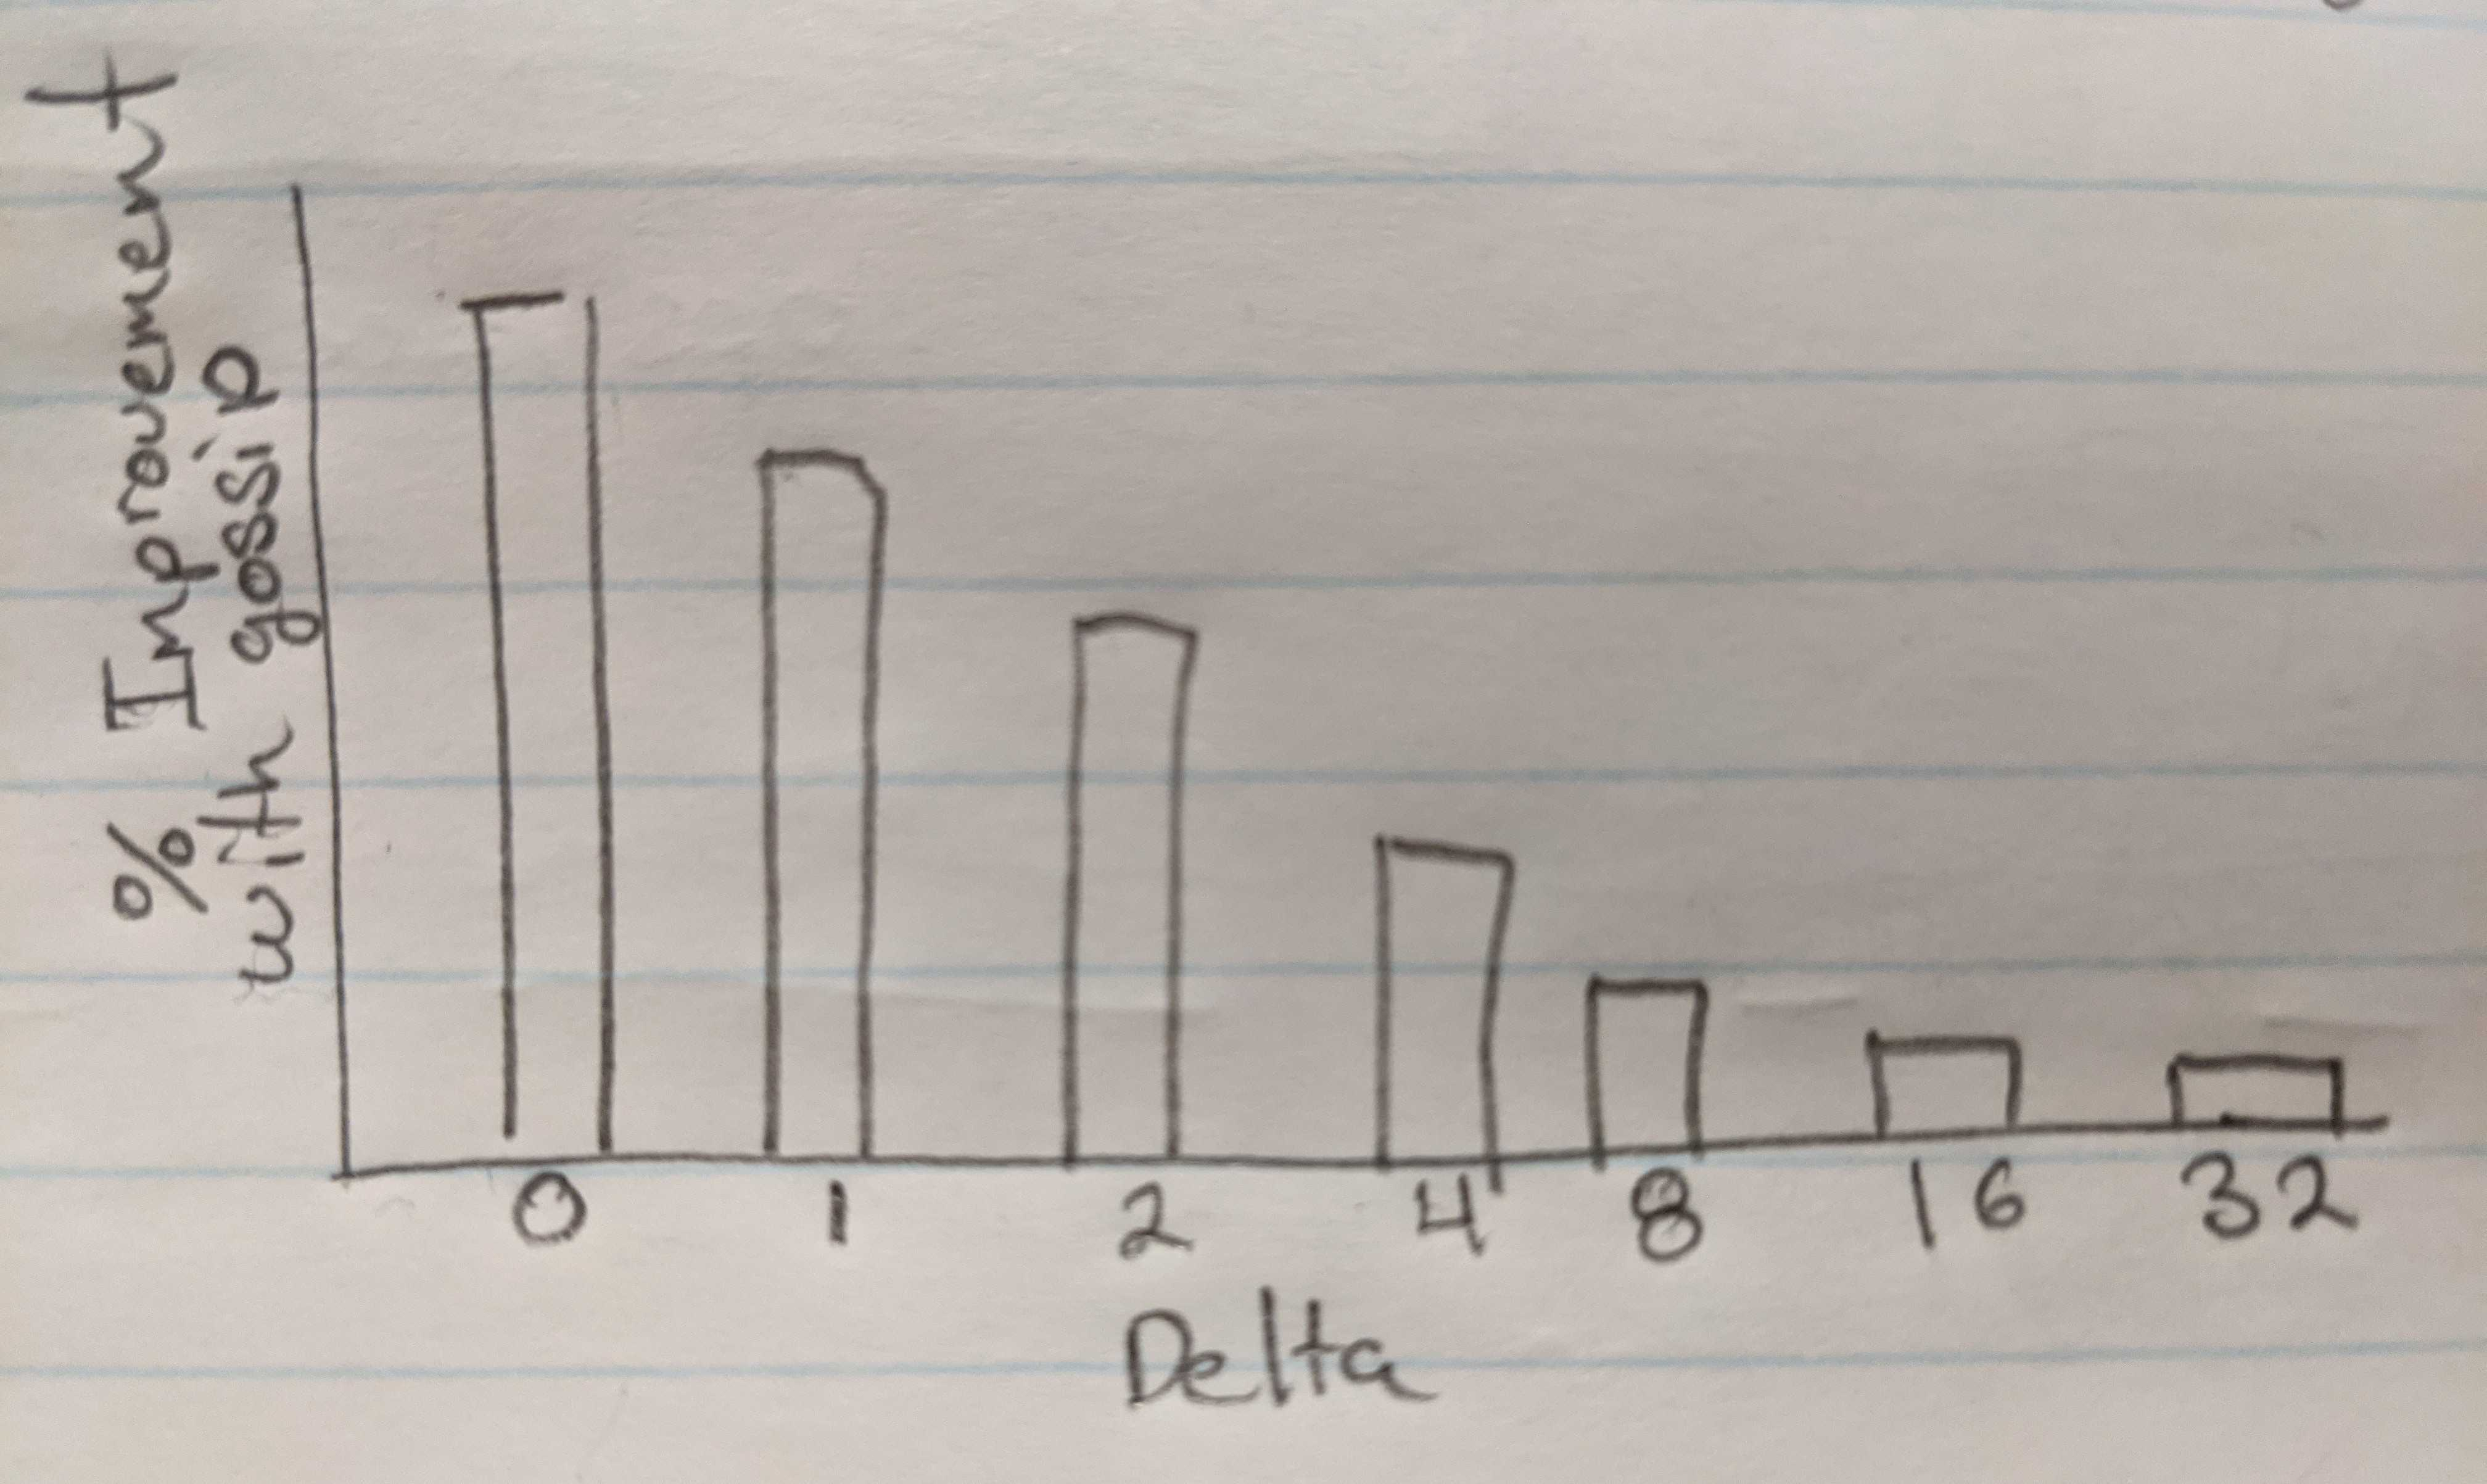
\includegraphics[width=0.45\textwidth]{fig/no_gossip.jpg}
%    \centering
%    \caption{\todo{Percentage improvement in load balancing decisions given
%%    50us load updates}}
%    \label{fig:no_gossip}
%\end{figure}

\subsection{Stale information}

The following experiments show that the frequency at which load is updated has a
significant effect on the quality of the decisions. 
%
However, there is a trade-off in terms of traffic overheads to keeping information up 
to date. 
%
As the number of services increases, so too does the number of messages needed to
keep the information fresh. 

Given imperfect, or stale, information about remote servers, the
question becomes: \textit{when is redirecting requests a good course of action}? 
%  
We submit that given reasonably predictable, but
potentially eccentric, request patterns, the correct course of action
is to act conservatively when conditions are manageable, and to react
quickly and decisively when request loads spike, i.e., in microburst
scenarios.  
%
These constraints dictate a compromise between inflating traffic and making sub-optimal decisions with poor information.

\subsection{Information traffic reduction} 

Determining how often and when to send load information requires
careful consideration. If an update were to be propagated for every
request, that would be ideal from a decisions making perspective, but
the overall number of messages sent could inflate by the total
replication factor (2$\times$ or 3$\times$ in many cases).  Such
overheads are unacceptable for systems with requests in the thousands
or millions of requests per second as the cost of the information
quickly surmounts the goodput traffic. A key challenge in designing a
distributed in-network load balancer approach is to identify the most
critical information to send which ideally only produces a small
overhead in terms of state exchange messages.

%\subsection{Predictability}

Network operators generally want predictable behavior within their networks.
Given that distributed load balancing requires information to be spread, it
raises the risk of adding unpredictability to the network, specifically in
terms of overhead. An ideal load-balancing strategy would spread information
efficiently while allowing operators to set an overhead budget in terms of
bandwidth or messages which would correlate to a comparable increase in
performance. Predictability is highly important in heterogeneous systems where
multiple applications require guarantees about their apportioned network share.

\subsection{Heterogeneous rack configurations}

At datacenter scale the configuration for any application may vary wildly.
Individual service replicas may be co-located with resource-hungry applications.
Due to configuration differences applications might have varying processing
powers. Many applications are placed in VMs which execute on differently
powered hardware. Indeed, in the datacenter there is no guarantee that any set
of replicas is equally provisioned. Therefore, any load-balancing strategy must
take into account this heterogeneity and apportion requests in response to the
real processing rate.

\section{Daronpon design}
\label{darapon:sec:design}

The \daronpon design resides within the ToR at each rack and is designed to
track server load by counting the number of outstanding requests for each
service running on that rack. Figure~\ref{fig:racks} illustrates the role that
ToRs play in our load balancing scheme.  When a request arrives at a ToR it
makes a load balancing decision. It either \textit{Admits} the request, or it
\textit{Redirects} it to another replica. The choice to either admit or
redirect is subject to the local load the service is currently experiencing
under the ToR (as understood by \daronpon), and an estimation of the load
each replica has on remote ToRs. 

%If a request is admitted the ToR increments it's
%load counter for that service. Once the server complete the request
%and the response from that service passes back through the ToR the
%load counter is decremented. Each TOR has a perfect count of the
%number of outstanding requests underneath it (assuming reliable RPC)
%which it can use to request count of services running on remote racks
%are sent periodically which give ToRs approximate knowledge of their
%load.  Using this information ToRs make the decision to \textit{Admit}
%or \textit{Redirect} a request when it arrives. 

A ToR can only directly keep an up-to-date counter for the services running in
its rack. To make good load balancing decisions, fresh knowledge, and more
importantly knowledge of bursty behavior, is necessary.  Determining the
mechanisms for disseminating this load information is non-trivial.

We designed and tested a variety of different options for disseminating load
information in simulation and on an Amazon Web Services (AWS) testbed.  One
design gossiped load information periodically based on wall clock time, and
another gossiped on a per-request basis. Our results in simulation and on our
test setup demonstrate that both of these techniques require extremely high
overheads in terms of messages sent.  For example, our best results with
periodic message exchanges required updates polled every 25us. This resulted in
over a 2x overhead in terms of messages. Most of the information spread in this
case was redundant, and does not aid in mitigating bursts.  Further, it adds
congestion to the network, which reduces the maximum throughput, especially
during bursts, which is the opposite of our goal. An ideal load dissemination
design would quickly react to bursts while simultaneously generating little
overhead during burst events.

\daronpon consists of two distinct but complementary messaging
mechanisms.  
%
The first mechanism is logarithmic gossip that guarantees the reactive spread of load information when bursts occur, 
while generating little overhead otherwise.  
%
The second one is opportunistic piggybacking that spreads load information between ToRs when requests are
redirected. 
%
We find in our evaluation that our log gossip approach prevents large queue build-ups, while our piggyback approach greatly reduces latency in the common case.  
%
%These results are outlined in detail later in this paper.

\begin{figure}[ht]
  \centering
    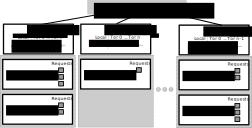
\includegraphics[width=0.8\textwidth]{./figure/daronpon/racks.pdf}
    \caption{High-level overview of \daronpon. Each ToR tracks
    outstanding request for services running in its rack, and
    maintains approximate counters for remote ToRs hosting shared
    replicated services.} 

  \label{fig:racks}
\end{figure}

%\subsection{Gossip Periods}
%\begin{figure}[ht]
%  \centering
%    \includegraphics[width=0.45\textwidth]{fig/diffgossip.pdf}
%    \centering
%    \caption{Different gossip periods from 1\/2 RTT to 16 RTTs. Using constant service time 25 us} 
%  \label{fig:diffgossip}
%\end{figure}

%Information about remote load counters is the key factor in making
%redirection decisions. Out-of-date load information is of low utility
%over time as its accuracy decreases. Therefore, the
%load gossip period has a remarkable effect on the overall performance.

%We tested the effect by running different gossip periods.
%After each run the period of gossip messages is doubled, starting at 25 us. 
%Figure~\ref{fig:diffgossip} shows the resulting
%trend when our servers are stressed at 30k request per second. 
%While doubling the gossip period, we can see 
%a linear performance degradation on 95th, 99th, and 99.9th percentiles latency
%starting at 100us, i.e. 1 RTT.
%The 50th, 95th, 99th, and 99.9th percentiles latency increase
%4.4\%, 26.9\%, 42.7\%, 58.3\% with 32x gossip periods. 

%%
%A marginal benefit is found at any gossip periods as a local redirections
%require a queue depths of 1 or greater, and even with poor information
%the probability of a redirected request landing at a less stressed
%server is sufficient enough for a performance benefit. 



% \sg{The aggregate number of gossip messages grows exponentially with the number
% of services running under each TOR. We should consider pointing out
% some mechanisms which might amortize the cost of these messages.}

% \begin{figure}[t]
%   \centering
%     \includegraphics[width=0.45\textwidth]{fig/load_spread.pdf}
%     \centering
%     \caption{ Request latency response to gossip message frequency
%     with servers loaded at 70\%. Exponential increases in frequency
%     lead to linear increase in performance. ~\todo{make off values
%     line up with ~\ref{fig:delta}} ~\todo{average over more runs, this
%     is taken over 10}.
% }
%     \label{fig:load_spread}
% \end{figure}

%\subsection{Load Delta}
%\begin{figure}[ht]
%  \centering
%    \includegraphics[width=0.45\textwidth]{fig/diffdelta.pdf}
%    \centering
%    \caption{Different load delta values to avoid aggressive redirection. Using constant service time 25 us} 
%  \label{fig:diffdelta}
%\end{figure}

%Figure~\ref{fig:diffdelta} shows microbenchmark results 
%of requests latency varies across delta values. 
%Applying ToR redirection with small delta values improves performance. 
%However, larger delta values avoid aggressive redirections but they hurt
%the performance by missing redirection with potential benefits.
%We can see the tail latency substantially increased after delta value of 10 under 
%a 35 KRPS request rate.
%The 50th, 95th, 99th, and 99.9th percentiles latency increase 
%23.0\%, 20.9\%, 13.3\%, and 12.5\% when delta value increase from 10 to 80.

%\begin{figure}[ht]
%  \centering
%    \includegraphics[width=0.45\textwidth]{fig/diffdelta0to10.pdf}
%    \centering
%    \caption{Zoom-in view of delta values from 0 to 10. Using constant service time 25 us} 
%  \label{fig:diffdelta0to10}
%\end{figure}

%As shown in Figure~\ref{fig:diffdelta0to10} increasing delta values
%from 0 to 10, we saw a smaller but observable increase on latency.  We
%observed 22.0\%, 19.9\%, 14.2\% increase on the 50th, 95th, and 99th
%percentiles latency.  The increase on 95th, and 99th percentiles
%latency starts at delta value = 5.

%We saw a local minimum of request latency at delta value 2 and 3 at medium request rate 30kRPS.
%Using delta=2 gives us 7.1\%, 8.2\%, 7.8\%, and 7.1\% improvements on
%on 50th, 95th, 99th percentiles, and 99.9th percentiles. Throughout
%our experiments we use a delta value of two as our local optimum.


%\todo{Load delta can be used as a way to reduce the total number of
%packet redirections. Should we choose to add redirections to the cost
%of our algorithm we want to show how using a load delta can decrease
%that}

\subsection{Microbursts}

Figure~\ref{fig:microburst} (top) shows an example of a microburst. In this
case, requests are issued at a Poisson arrival rate by multiple clients.  The
peaks show outstanding requests from the perspective of a ToR instrumented to
track request counts. In this case, when requests queue, that queue grows
without bound, even though other replicated services are available to process
this influx of requests. This has a dramatic impact on the tail latency of the
requests in the burst, and also the overall mean request time. A typical
request incurs longer wait times due to decreased overall system throughput.

In Figure~\ref{fig:microburst} (bottom) the queue builds up with our
logarithmic gossip mechanism enabled. Each \textit{red X's} on the chart
represents a point at which the load on the server is gossiped.  Note that when
peaks occur, and a gossip is sent, the load is quickly spread to other servers.
This increases overall system throughput and decreases tail latency. This
strategy, however, is not perfect. At low load the benefit of redirecting
requests is minimal. For example, when the number of outstanding requests is
just one or two above a remote service, and so redirection reduces overall
performance.

The age of the gossiped information complicates the act of redirecting. The
remote information on remote hosts is at least a few microseconds out of date.
Given the few microsecond budget our requests have to begin with, the benefit
of redirection quickly evaporates if even a few requests arrive from the point
in time at which the load information is sent.  This leads to unnecessary
redirections and high overheads in terms of gossip messages which do not
ultimately deliver useful information. This overhead can be mitigated by adding
a threshold which prevents gossip messages from being sent until the number of
outstanding requests has exceeded a given threshold.  Our proposed log gossip
technique for curtailing this overhead is described in the following section.

%Gossip messages consume and packet processing time.  Therefore their
%frequency must be chosen with care as to not introduce significant
%variance into the system. The majority of data center packet drops
%occur on south facing ToR egress to the host.~\cite{jupiter-rising},
%our approach only increases bandwidth above the ToRs which allows for
%a higher gossip bandwidth budget prior to it causing significant
%interference. Gossip messages are small, (approximately
%64 bytes depending on the number of services), which reduces aggregate
%bandwidth consumption.

%Our testbed results use gossip messages as
%frequently as 10us without any noticeable interference on 40Gbps
%networks. As network speeds increase we anticipate that the available
%bandwidth for background traffic which improves the performance of
%running services will increase.


\begin{figure}[t]
  \centering
    \includegraphics[width=0.80\textwidth]{./figure/daronpon/burst.pdf}
    \centering

    \caption{Microburst with no mitigation (top) vs. with
    logarithmic gossip load balancing enabled (bottom)}

  \label{fig:microburst}
\end{figure}

\subsection{Packet flow}

The \daronpon\ load balancers are stateful and act per request.
Figure~\ref{fig:load_balancer} provides a high level message flow diagram of
this system.  When requests arrive, \daronpon executes the admission
protocol. Requests are admitted only if the local service has the minimum
observable global load. A load tracker keeps counters for each global service.
Local counters are up-to-date, while remote counters are learned via gossip and
piggyback messages.  When a request is admitted, the ToR increments its load
counter corresponding to that service.  When a response passes back through the
ToR, that service has its local counter decremented.  If, when a request
arrives, the local load of a service is not the global minimum, the request is
redirected. The redirected request is then sent to the service with the lowest
load, based on the ToRs' local load tracker (see
Section~\ref{daronpon:sec:design:piggyback}).  Redirected requests have load information
attached to them. The attached load consists of request counters for the
intersection of services the ToRs share.  Therefore, the overhead per
redirected request is variable as per the systems' configuration.

Increments and decrements in local load are tracked by a gossip monitor (see
Section~\ref{darapon:sec:design:gossip}). The job of the gossip monitor is two-fold. First,
it identifies bursts. When load spikes the monitor broadcasts gossip messages
to let other ToRs know it is experiencing high load. Second, it identifies
valleys. Load balancing schemes which use potentially stale information are
known to exhibit herding behavior, a condition which leads to sub-optimal
queuing behavior~\cite{dahlin_stale_info,mitzenmacher_old_info}. When load
drops sharply, gossip messages are also generated to announce that a service
has spare processing capacity.

\begin{figure}[t]
  \centering
    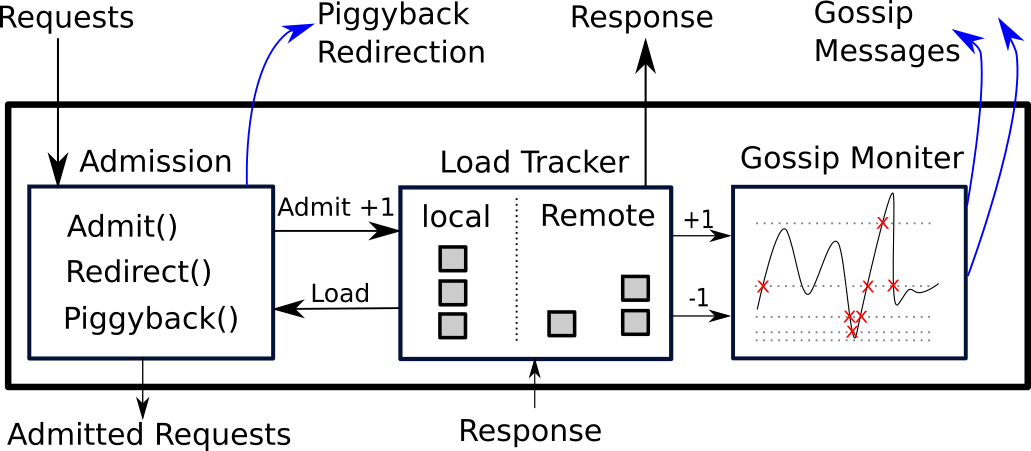
\includegraphics[width=0.80\textwidth]{./figure/daronpon/load_balancer.pdf}
    \centering

    \caption{ %% 
        %%
        Key functionality and message flow of \daronpon.
        Incoming requests are either admitted or redirected.
        Redirected requests spread load information via piggyback.
        Load is updated upon admission, and response.  Gossip messages
        are issues when load breaks a logarithmic threshold.}

  \label{fig:load_balancer}
\end{figure}

\subsection{Logarithmic Gossip}
\label{darapon:sec:design:gossip}

\begin{figure}[t]
  \centering
    \includegraphics[width=0.90\textwidth]{./figure/daronpon/log_thresh.pdf}
    \centering
    \caption{The percentage of gossip messages generated by a
    logarithmic gossip mechanism as a percentage of overall traffic.
    Collected from runs of 96 KRPS.} 
  \label{fig:log_thresh}
\end{figure}

\daronpon generates gossip messages aiming to reacting quickly to bursts while consuming little overhead in terms of additional messages.  
%
In an earlier design, ToRs gossiped load information every 25 $\mu$s. 
%
This logarithmic gossip approach has the advantage of providing highly updated load information, but it incurred scalability bottlenecks as the number of ToR increased, since the 25 $\mu$s gossip contends with request goodput for link bandwidth.

To compress the number of messages, \daronpon's gossip messages are sent
on exponential changes in load. 
%
\daronpon uses powers of two as the interval. 
%
\daronpon chooses two for its ease of computation requiring only bit shift operations because no commodity programmable switch, to our knowledge, is able to compute floating point arithmetic~\cite{challenging_programable}.
%both for its effectiveness in practice and 

Each step increases the bounds in which server load can fluctuate
prior to a gossip message being issued. 
%
For instance, if the load were to
increase from 1 to 2, a gossip message would be broadcast to all other servers
with the replicated service that crossed this threshold.
%
In this message, load information for all other shared services is added. When the boundary of two is crossed, and the value of two is sent, this ToR will not issue another gossip message until the load on the service rises by a power of two to four, or falls back down by a power of two to one.

%%
%% Sorting microbursts by size
%%
Logarithmic gossip has several benefits. 
%
First, it sorts microbursts by magnitude without adding significant packet overhead. Given that small fluctuations may occur at rapid pace, it is important to give priority to bursts with larger magnitudes.
%
% Other methods of achieving this goal such as piggybacking can lead to stale information, which has significant differences to ground-truth values, even when a server is experiencing very high load.


%%
%% Reduces congestion when bandwidth is needed
%%
Second, logarithmic gossip reduces the number of gossip messages sent during 
bursts, which reduces the overall strain on the system when resources
are at their tightest. 
%
This is an issue with gossip strategies that operate periodically (e.g. at preordained wall clock times) or are issued at some constant ratio
to requests (e.g gossip every 5 requests). 
%
When request rates are low, gossip messages are automatically sent with a higher frequency per number of requests which allows for better decision-making at lower
request rates.
%%
%%Aggregation of requets
%%
ToRs have the advantage of being an aggregator for the load of an
entire rack. 
%
Were we to implement our solution on end hosts, each host
would need to gossip its load to every other host. 
%
Using ToRs, the load of each server in a rack is known explicitly and is gossiped in its entirety, assuming the rack sees both requests and the associated
responses.

%%
%% Fast reaction
%%
Other approaches which use load information collected from end hosts
themselves suffer from additional delays in responding to load spikes,
as the knowledge of load must be transmitted to the balancer before it
can react. \daronpon's logarithmic gossip mechanism reacts to load as soon as a request is admitted. 
%
This allows for precise load balancing decisions to be made at sub-RTT time scales. 
%%
For instance, in a Fat-Tree with two ToRs connected by a single
aggregate switch, the distance traveled by load updates is halved in
comparisons to a host based solutions (e.g. Tor-Agg-Tor vs
Host-Tor-Agg-Tor-Host). This approach is not limited to Fat-trees,
as many networks use ToRs, however our ToR-based approach always results
in two hops less than an host based approach.

%% %Approximate measure of load, but fast react %
\daronpon's logarithmic gossip estimates server load on the ToR with counters instead of  requiring precise and up-to-date measures of load on the host, which we can
only get with precise application level knowledge and host control, 
%
This imposes lower tracking overhead, and performs nearly as well as highly tuned approaches which report server load directly~\cite[Figure. 15 (proactive)]{racksched}.
%%
%% Threshold
%%
This algorithm decreases the number of gossip messages
significantly, and can be greatly improved by carefully considering a
lower bound at which to disable the mechanism entirely.
For example, setting a lower threshold such as $t$ implies that below an outstanding request count of $t$ a ToR will not gossip information.
%
The threshold is determined by an exponential weighted moving average and a floor value that the threshold does not go beneath it.

Figure~\ref{fig:log_thresh} shows the percentage of messages gossiped relative
to the requests processed for different threshold values.  Note that the
default values of 0 and 1 have an overhead of around 30\% of the request rate.
Redirections of requests at these levels of outstanding request sees little
benefit in terms of performance as at any reasonably high request rate, the
depth of remote queues have changed since the remote data was received making
the choice stale. 
%
By increasing the threshold to four, the overhead in gossip
messages is reduced by a factor of ten down to around 2\% when our system is
around 70\% saturation. 
%
This suggests four is a good floor value for the gossip threshold setting.
%
See Section~\ref{sec:service_time} for a comprehensive
evaluation of gossip overhead. Increasing the gossip threshold beyond four
significantly reduces overhead down to around 0.02\%, however this comes at the
cost of only identifying bursts of size eight and greater which significantly
effects our reductions in 99th percentile tail latencies.

%%
%% Staleness
%%
Logarithmic gossip, however, provides no liveness
guarantees to the freshness of the load information announced despite all the aforementioned benefits. 
%
For instance, a server which maintains an outstanding number
of requests between 4 and 16 for $n$ requests will not issue a gossip
until either threshold is crossed. While this is unlikely in practice
due to the small range and short duration of requests, there is no
guarantee. This can become an issue for extended periods of load when
the number of outstanding requests is deep (e.g. 128 to 512).

\subsection{Piggyback}

\label{daronpon:sec:design:piggyback}
\begin{figure}[t]
  \centering
    \includegraphics[width=0.90\textwidth]{./figure/daronpon/breakdown.pdf}
    \centering
    \caption{Performance breakdown of gossip and piggyback mechanisms.
    Lower values are better.} 
  \label{fig:breakdown}
\end{figure}

Beyond using logarithmic gossip, the redirect requests also able to propagate load information by making load information riding with these requests heading to remote ToRs.  
% Using logarithmic intervals for gossip messages, we can identify and
% mitigate bursts.  
%
% Logarithmic gossip propagates load information, when the intervals are met, to remote ToRs, but the opportunities provided by redirected requests is untapped. 
% While this is advantageous in general, there is still
% additional performance to be gained.  
%
With gossip enabled, the percentage of redirected requests is 22\%. 
%
Each of these redirected requests is sent from the redirected ToR to the receiving one, and therefore has the ability to report the load information on the ToR that performed the redirection.  
%
We refer to this method of attaching load information to
redirected requests as piggyback, and using redirection to spread information
provides significant advantages in the common case.
%
Piggybacking depends on a threshold called load delta indicating the difference 
between the load on local replica and the load information on remote replica.
%
Load delta determines the triggering of redirection and controls the aggressiveness of redirection.
%
It is determined by an exponential weighted moving average as a threshold to adapt for different workload patterns.

In contrast to the centralized approaches in both Racksched and
R2P2~\cite{racksched, r2p2} piggybacking information load on requests
is not a sufficient mechanism for learning about remote load. This is
because our load balancer is decentralized, which means that our load
balancers do not see load information updates from every request.
Unlike our logarithmic gossip mechanisms, it provides no guarantees
about its operational bounds. Using gossip messages exclusively
provides no guarantees that any specific server will have information
propagated to it as only the server which is redirected to receive
fresh information.

In the case of these centralized solutions, each request returns some
information to the scheduler. In the distributed case, there is no liveness
guarantee with regard to redirections, and indeed, information can become
arbitrarily stale. We therefore consider our piggyback algorithm to
opportunistic, only aiding in the common case when load is low, but when making
precise redirections will still improve throughput and provide
lower latency.

Piggybacking load has the advantage that it is responsive proportional to the
request rate of the system. 
%
As the number of requests per second increases so to does the rate at which information is spread between ToRs. 
%
Furthermore, it has the advantage of introducing a small amount of overhead. Rather than incurring the cost of an entire load information update, this only adds a few bytes to a custom header injected at the ToR.


Figure~\ref{fig:breakdown} shows a performance breakdown of the two pillars of
\daronpon's design: logarithmic gossip and piggyback compared to a baseline of performing random selection on the client alone. 
%
At low request rates the logarithmic gossip does not provide much of a performance benefit in relation to the piggyback method. 
%
However, as the request rate, and variability, of the system rises (e.g. to 102 and 105
thousand requests per second), the logarithmic gossip provides the majority of
the gains as it detects the peaks which increase tail latencies the most.

\section{Implementation}

We deployed \daronpon on the AWS cloud with instances hosted in VMs connected via Elastic Network Adapter (ENA) virtual NICs. 
%
These instances use the Data Plane Development Kit (DPDK).

\paragraph{Components:} Our deployment consists of three components: DPDK ToRs,
DPDK clients, and servers with default Linux networking stacks relying on UDP
for application messaging. DPDK is a kernel bypass networking library which
allows for high throughput and low latency packet processing in user
space~\cite{dpdk}. DPDK ToRs emulate ToR switches with limited latency overhead
($<$ 1 microsecond).  Ideally, we would implement our algorithm on P4 switches,
however to our knowledge no cloud providers allow for customers to offload
custom programs to programmable switches at this time.  We implement our
clients using DPDK for lower latency and precisely controllable request rates.
These traits are important as AWS's ENA NICs do not have hardware timestamping
available to users.  Our DPDK clients can generate hundreds of thousands of
requests per second with a single virtual core. These UDP-based servers
represent services relying on the standard Linux networking stack. We choose to
use UDP as the transport because it allows us to redirect request atomically
without connecting multiple packets together and redirecting as a group, though
this could be supported as future work.

\paragraph{\daronpon\ DPDK ToRs:} DPDK ToRs use an arbitrary number
of cores to forward requests/responses and a single core to gossip
load information. Redirecting involves header manipulation, tracking
load information using hashtable table lookups, and counter
increment/decrement operations. The operations we used in these DPDK
ToRs are carefully chosen to be simple, and within the capabilities of
programable switches to compute.

\paragraph{Custom packet headers:} \daronpon appends a custom header after
the IPv4 UDP header. The header consists of a unique request ID for each
request, which is used to track lost packets and measure end-to-end
latency. A service type field differentiates services, e.g. Memcached
and RocksDB.  Additionally, the IP and ports describe addresses of
replicas which implement other copies of the service.  We assume that
clients know the server replica addresses by asking the cluster-level
replication manager, e.g., Google's Slicer or Facebook's Shard
manager~\cite{facebook_shard,google_slicer,microsoft_service_fabric}.
Gossip messages are also based on UDP, and load information is
appended after the UDP header.  The header contains a list of server
addresses, load counters, and its corresponding service types for all
servers under a ToR switch. 

\section{Evaluation}
\label{daronpon:sec:eval}

%define setup variables here
\newcommand{\racks}[0]{3\xspace}
\newcommand{\services}[0]{2\xspace}
\newcommand{\servers}[0]{6\xspace}
\newcommand{\servercores}{1\xspace}
\newcommand{\tors}{3\xspace}
\newcommand{\torscores}{16 \xspace}
\newcommand{\clients}{6 \xspace}
\newcommand{\clientcores}{1 \xspace}

We evaluate \daronpon in on the Amazon Web Services cloud (AWS
\texttt{us-west-2} region) using \texttt{c5n} instances. 
%
In this section, we describe the experiments and the resulting conclusions.

\subsection{Experimental Setup}
We use \servers instances as servers, \clients as clients, and
\tors as software ToRs. 
%
All instances are placed in a cluster placement group for predictable low latency. 
%
The mean RTT latency between every instance is 50 microseconds. 
%
In this setup, we configure \servers servers, \clients clients, and \tors software ToRs. 
%
This configuration emulates a datacenter network of \tors ToRs that each ToR has \services services running underneath it.  
%
Services are deployed to servers using the stock Linux networking stack.  
%
While this does incur higher latencies as compared to DPDK-based kernel bypass stack, we note that it is representative of many datacenter applications.

We implement the \textit{random} and \textit{Power-of-2 choices} as the baselines. 
%
Both of them select the replica of the service on the client side. 
%
\textit{Random} baseline selects a replica of a service regardless of any load information.
%
\textit{Power-of-2 choices} for service selection is another baseline that selects a replica of a service based on load information available to the client.
%
The power-of-2 choices~\cite{power_of_2} randomly chooses two random replicas of services and picks the one with lower load out of the two ones.   
%
The load information used for service selection is stale when it reaches the client because the actual load may have changed.
%
The load information is obtained with active probing the servers or from the response of a previous request.
%
% This load creates unnecessary congestion on the DPDK ToR instances and
% ENA virtual NICs.  
% \daronpon\ can be easily extended to implement the ``power
% of two'' approaches on ToRs and the performance should be similar, based on
% simulation results reported in LSQ~\cite{lsq}.  
% Each client randomly selects a service designation. 
% In the random configuration, requests traverse our DPDK
% software ToRs with our load balancing mechanism off, and they flow through to
% their selected destinations. 
%
We compare \daronpon to random and power-of-2 choice in
the experiments.

\subsection{Workloads}
%
We evaluate our load balancing approach with request-response based 
applications, in which the time spent on the server is emulated based on 
different statistical distributions.
%
In our evaluation, we generate requests according to two
statistical distributions, one of which generates application-level requests
and is run on DPDK-based clients, and another which generates emulated service
times. 
%
Clients generate requests based on open-loop Poisson arrival using the
standard random library.  
%
Servers distributions are split into different distribution categories, each of which has its own separate parameters. 
%
These include constant time, bimodal, and exponential distributions. 

Each server is loaded with an equal number of requests (in expectation)
drawn from common request rate distributions, as described next.
Our goal in using these distributions is to demonstrate that
using outstanding requests (blind to the underlying
service distribution) works in general, without the need to tune
our load balancer for each application.  
%
Both our gossip and piggyback mechanisms are enabled in each experiment. 
%
The lower threshold on the gossip mechanism is initialized as 4.

\noindent\textbf{Constant:} In this configuration, all requests compelte in 25 $\mu$s on the server.  
%
On the server, a work thread busy-polls the time until 25 $\mu$s has passed to emulate application-level service times.
%
This type of workload is indicative of many highly tuned key-value stores with strict
SLOs~\cite{memcached,rocksdb}.  
%
The servers experience additional latency overheads from the Linux networking stack.  Our choice of this constant latency is intended to be representative of a performance-tuned microservice which performs a fixed amount of work per request. 
%
To provide a sensitivity analysis to this choice of constant, Section~\ref{sec:service_time} provides an overview of \daronpon's performance across constant service times 
%
%separated by an order of magnitude above and below 25us.

\noindent\textbf{Exponential:} To generate an exponential distribution we use the
standard C++ random library. We set the mean to 25 $\mu$s with a standard
distribution of 40,000. These parameters generate tails of up to 400 $\mu$s
which is indicative of many applications that may be subject to blocking, such
as occasional writes to disk or the invocation of a blocking RPC to another
machine.

\noindent\textbf{Bimodal:} Our bimodal service times are distributed into two
categories. 90\% of the requests take 13 $\mu$s and 10\% are 130 $\mu$s.  We
choose this distribution as the mean value is close to 25 $\mu$s. This
distribution is aimed at emulating longer and less frequent tasks such as
writes and scans in certain key-value store workloads or even garbage
collection events in the runtime.

\subsection{End-to-end experiments}

\begin{figure*}
  \includegraphics[width=\textwidth,height=4cm]{./figure/daronpon/homo.pdf}
  \caption{99th percentile latency improvements on three common
    service distributions (Constant, Bimodal, Exponential). Each
    server is provisioned with homogeneous processing power.}
  \label{fig:homo}
\end{figure*}

We test the effectiveness of our load balancing technique by running it against
random replica selection alternatives on the aforementioned workloads.
Figure~\ref{fig:homo} shows the relative performance gains across these
workloads at the 99th percentile latency. In this configuration, each of the
servers has identical processing capacity for each service.  We consider this
idealized and homogeneous configuration because of its simplicity.

\daronpon demonstrates the most relative gain over random when skew in the workloads
is common. At high loads, request variation occurs at higher degrees for
multiple reasons. First, the Poisson arrival process on our clients has a
higher probability of generating bursty sequences of events at higher load.
Second, hypervisor and NIC hardware on AWS contributes to the bursty arrival of
requests because of the underlying batching behavior.  These forms of
burstiness is largely out of our control as we do not have direct access to
AWS's hardware configuration.  Finally, as rates increase, more batching
happens in the Linux kernel networking stack. This leads to sharp decreases in
the number of outstanding requests. 

\daronpon demonstrates observable benefits in the bimodal and exponential
distributions and the long service times cause significant and frequent queuing
on the end hosts. \daronpon's logarithmic gossip design reacts quickly to these
changes under load and steers requests away from the servers which are running
long average request times.  In our homogeneous experiments, the average value
for number of outstanding requests is four in our constant distribution, with
frequent peaks of up to 80 outstanding requests when \daronpon\ is disabled.

\noindent\textbf{Constant:} Figure~\ref{fig:homo}-left shows our approach provide benefit
on tail latency starting at 1248 Krps (kilo-requests per second).  This constant
workload gives \daronpon\ the fewest opportunities to load balance effectively
as the random distribution of requests, each with a static service time, should
be approximately even. In this distribution, the benefit is found in the load
fluctuations. At high request rates, other mechanisms such as Linux's request
batching, have more of an effect on queuing.
%
At the highest request rate that a single vCPU core can handle, the latency
improvements of \daronpon over the random and power-of-2 choice baselines are 
0.60 $\times$ and 0.25 $\times$ at the 99th percentile with the highest request rate. 
%
The improvement over power-of-2 choices is less because the evenly distributed requests given the same constant service times. This remediates the stale information and makes the performance of power-of-2 choices relatively close to \daronpon.    

\noindent\textbf{Exponential:} Figure~\ref{fig:homo}-middle shows the throughput and
latency gains on an exponential server distribution. The benefits are most
noticeable here as the exponential distribution leads to the fastest disparity
in load. In this case, a single request on the exponential distribution can
lead to significant queuing on a given server. 
%
\daronpon's latency improvements over the random and power-of-2 choice baselines are 
0.54 $\times$ and 0.43 $\times$ at the 99th percentile. 

\noindent\textbf{Bimodal:} In Figure~\ref{fig:homo}-right, we see the disparity between
random service selection and \daronpon. The service time dispersion provided by
bimodal distribution causes noticeable request queuing when a long service time
request occupying a service.  
%
Logarithmic gossip messages are ideal in this case as they quickly react to the skew in load.  
%
Further, in this distribution the probability of finding an under-utilized replica is relativity high.  
%
The difference of 99th percentile latency between random and power-of-2 choices shrinks compared to the case of the constant and exponential service time. 
%
The 99th percentile latency of power-of-2 choices moves closer to random as the queuing penalty of selecting the congested replica could be as large as 130 $\mu$s.  


\subsection{Heterogeneous server configurations}

\begin{figure*}
  \includegraphics[width=0.9\textwidth,height=4cm]{./figure/daronpon/hetero.pdf}

  \caption{Throughput and latency improvements with skewed processing
    capacity in a heterogeneous server configuration. \daronpon\
    scales linearly with with the aggregate processing capacity
    available.}

  \label{fig:hetero}
\end{figure*}

The placement of replicated services is subject to the cluster
scheduler~\cite{facebook_shard,google_slicer,microsoft_service_fabric}.  The
placement of individual services may be tightly coupled to a single rack, or
distributed to multiple racks. Additionally, not all replicated services may be
configured using identically powered instances. Some may be provisioned with
different core counts, memory, and potentially different OS versions.  Finally,
should rack-level scheduling be utilized such as Racksched or R2P2, the
individual rack level throughput may differ below the operating domain of \daronpon.

To show the generality of our approach in situations where replicated
applications differ in their throughput capabilities, we configure one out of
our three servers to run using three times the processing capacity, i.e., 3 $\times$ number of CPU cores rather than one. In this setup, clients otherwise operate identically to
the homogeneous configuration.

Figure~\ref{fig:hetero} shows the performance gains from enabling \daronpon on
our heterogeneous testbed. In this test, the server with twice the processing
power of the other processes requests twice as quickly.  Our random client
takes no measure of queue depth, and therefore does not adjust to this excess
compute power. Its performance is only marginally better in this case, as the
request which it probabilistically sends to the doubly provisioned server are
processed more quickly. 

\daronpon apportions load to servers in precise relation to their processing
power. Our results from this test show that \daronpon exhibits good scaling with more computation in this configuration. 
%
\daronpon is able to process 1.4 $\times$ in the case of the constant service time.
%
When running in a heterogeneous configuration, the proportion of gossip and piggyback
request remains approximately the same as in the homogeneous case. The gossip
mechanism is triggered periodically as the request on the faster servers drains
below its current threshold, however this periodic variance occurs on the same
order as the natural fluctuations in load. Redirections also occur at
approximately the same rate, however they are almost entirely directed at the
over provisioned server.

Ideally, we would demonstrate the scalability of \daronpon across many racks
with more services. We see this heterogeneous result as a proof of concept that
our approach can scale approximately linearly with available processing power.
We expect this result to hold as our approach is similar in style to
theoretical approaches for distributed load balancing which are proven to
provide linear scaling while using incomplete local information to balance
load~\cite{lsq}.

\subsection{Gossip and Piggyback Overhead}
\label{sec:service_time}

%\label{sec:service}]
\begin{figure}[ht!]
  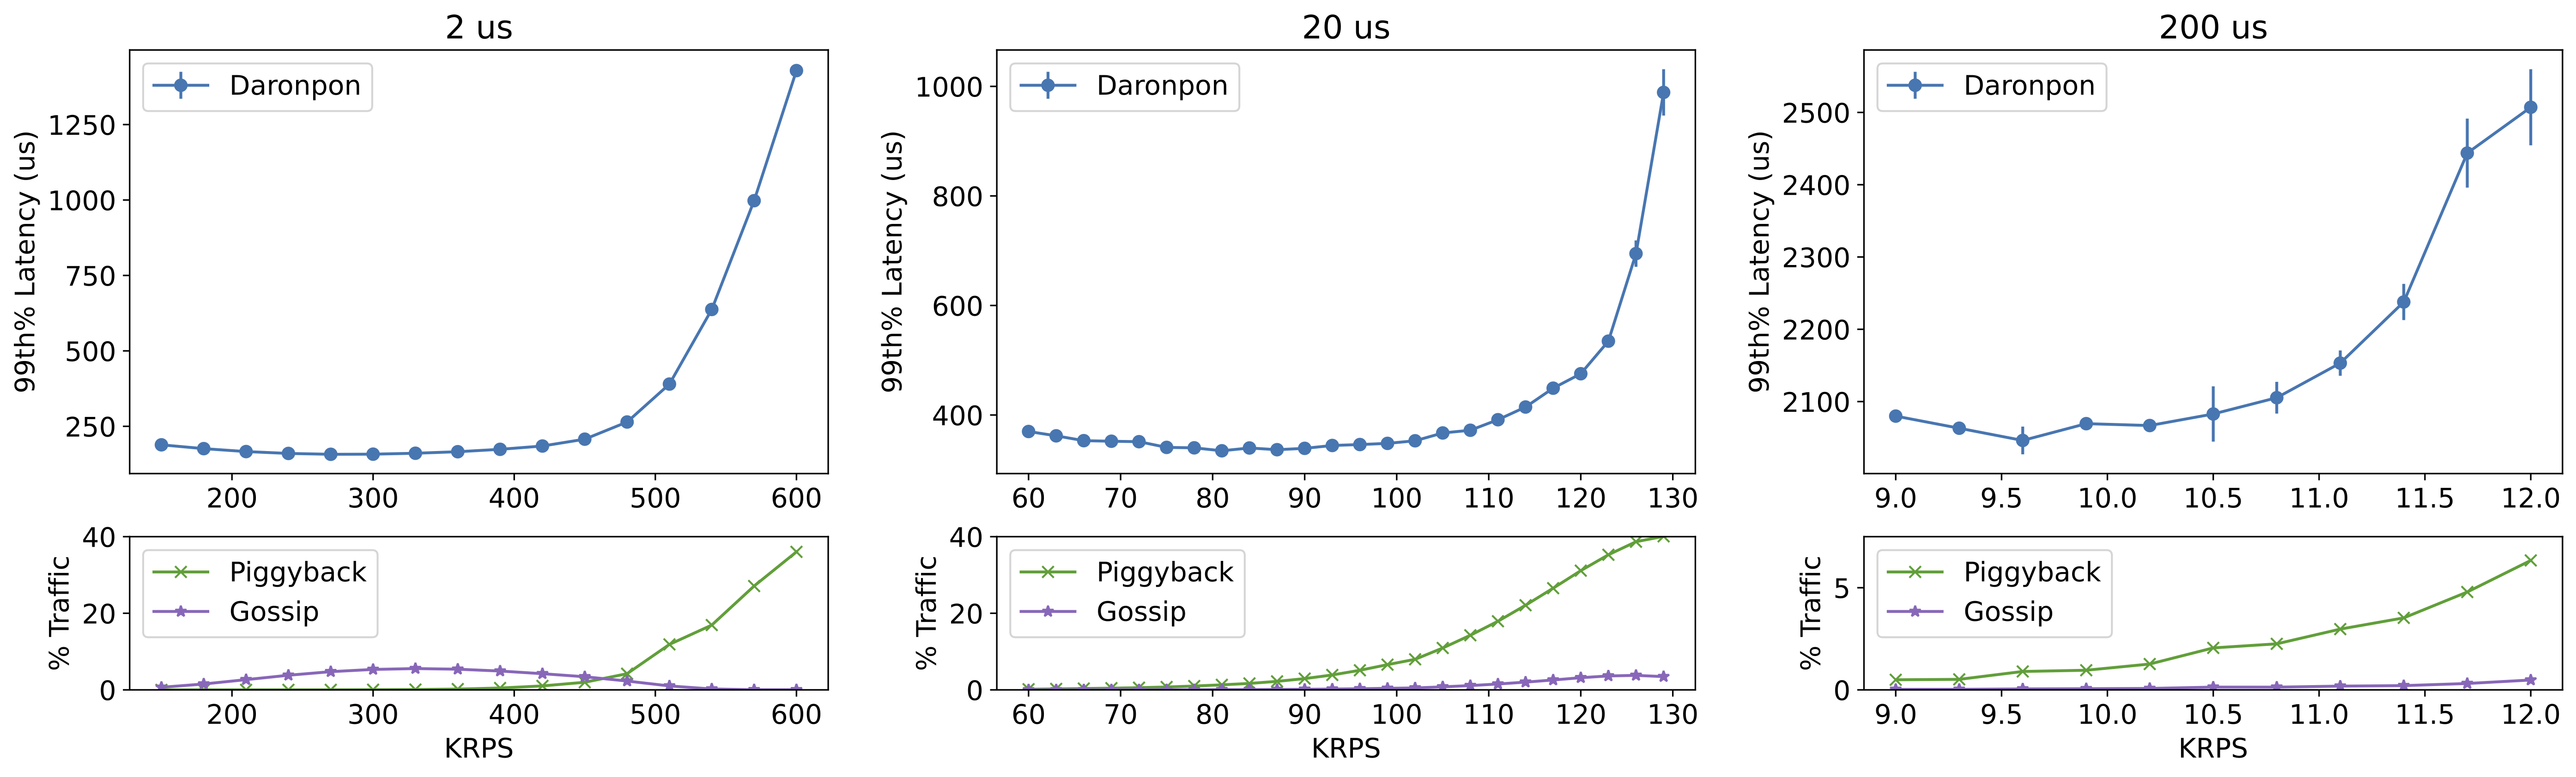
\includegraphics[width=\textwidth,height=4cm]{./figure/daronpon/service.pdf}
    \caption{Service times across three orders of magnitude (2us, 20us,
    200us). \daronpon\ provides relative improvements with similar
    overheads in terms of piggyback and gossip messages at each
    service time.
    }
  \label{fig:service}
\end{figure}

% \stingw{It should be 20 us instead of 25 us in the writing except we try to talk about 
% the baseline we did in the previous experiment}

To investigate \daronpon's sensitivity on service time and the related overhead, 
we vary constant service times by three orders of magnitude across three experiments: 2 $\mu$s, 20 $\mu$s, and 200 $\mu$s.  
%
This helps us to understand the overhead of our logarithmic gossip mechanism, the redirected proportion of messages with piggybacked load information under different service times. 
%
First, constant service times stress the servers more because it makes the servers
to process more requests per second.  
%
With more incoming requests, the number of outstanding requests 
on the switches is also higher.
%
Second, we set up aggressive redirection that does not require the load of a remote replica to be lower than that of the local one.
%
In this experiment, the load delta between remote and local replica is set to 0, which means that the minimum replica is always selected regardless of the performance impact.
% we devise a threshold similar to the baseline used in our log gossip mechanism which required the value of a remote queue to be lower than that of the local queue by a specified delta before redirection.
%
Choosing delta above 0 resulted in a lower number of redirections, with a delta of 8 resulting in piggyback messages being generated for only 6\% of all requests.
%
The aggressiveness of redirection is a trade-off of performance, resulting in lower tail latencies at the cost of the bandwidth.

Figure~\ref{fig:service} shows the tail latency and the corresponding overhead 
of \daronpon.
%
%\stingw{We can show this in paragraphs instead of drawing the random lines again!}
% At 2 $\mu$s, \daronpon\ provides 52\% and 41\% less improvement over the random and power-of-2
% ~\TODO{Pending definition} baselines compared to its 25 $\mu$s counterpart.
%
At 2 $\mu$s (Figure~\ref{fig:service}-left), the 99th percentile latency increases wit higher request rate as expected.   
%
Interestingly, \daronpon gossips more frequently between 200 and 400 Krps and shows a bump peaks at 330 Krps.  
%
The frequent trigger of gossip is because gossiping thresholds are based on power of two numbers, e.g. 2, 4, 8, 16, etc.    
%
Statically, gossiping thresholds are more frequently met when the number of outstanding requests is lower.
%
For example, an increase of outstanding requests from 1 to 8 triggers 3 gossip messages while an increase from 8 to 17 triggers a single message.
%
At ranges of 64 and above, \daronpon gossips when encountering bursts of incoming requests.
%
\daronpon gossips less frequently during higher request rates when piggyback takes over gossip as the main mechanism to propagate load information.

At 20 $\mu$s (Figure~\ref{fig:service}-middle), \daronpon
operate with the maximum gossip overhead reaching no more than 3\% at peak system load. 
%
On the other hand, the number of piggyback messages grows with the request rate. 
%
This is because at higher rates more bursts occur, and thus the opportunities to load balance increase.
%
Near peak load, piggyback messages reach approximately 40\% with the highest request rate, 
the redirected packets do incur additional bandwidth usage.
%
The additional uplink bandwidth usage, as mentioned in Google's Jupiter-Rising paper~\cite{jupiter-rising}, does not stress the most bottleneck links that are all downlink to servers and to ToR switches. 

At 200 $\mu$s service times, \daronpon operates with lower traffic on piggyback as the service time is longer.
%   
With longer service time, it provides a larger window for load information to propagate. 
%
The overhead from gossip remains low. 
%
%When request rates are high, latency shows higher variance because 
%
% is largely improved from the increase in redirected messages which provide ample fresh load information which allows for more accurate predictions of the globally shortest service queue.

%provides better performance
%relative to the 25 $\mu$s as information on the servers is likely to stay fresh
%for longer due to the decreased request rate.  
%
%The latencies at request rates lower than 9 Krps are higher because interference from the Linux kernel which
%starts to reschedule cores below that threshold~\cite{mutilate}.

\section{Discussion}
\label{darapon:sec:discuss}

\paragraph{Scaling:} In production cluster, managers determine the application
service replication factor. This factor is determined dynamically by monitoring
system load, which can cause applications to scale up and down significantly on
the order of hours.  \daronpon{}'s gossip broadcast is inflated by this
replication factor, and therefore very large replication counts (e.g. in the
100s) present a potential bottleneck.  We believe that overhead can be
constrained with proper placement of services to maximize the intersection of
services across a same set of racks.  Additionally, careful placement enables
piggybacking to carry more load information per redirected request.

\paragraph{Emerging Topologies:} \daronpon\ works on any datacenter topology
which uses ToRs, or virtual ToR-like abstractions (such as our DPDK software
middlebox switches). Emerging network designs, e.g. Jellyfish~\cite{jellyfish}
and Xpander~\cite{xpander}, are supported under our architectural assumptions.
Some network designs have asymmetric latencies between servers.  While this may
cause some racks to propagate information which is more stale, we do not see
this as a limitation of our techniques as our AWS testbed has latency variations
on the order of a few microseconds.  \daronpon's redirection piggyback and load
gossip can take a variable amount of time to propagate load information to
other ToRs, but our load balancing design is similar to theoretical techniques
prevent to be effective even with stale information~\cite{lsq}. 

\paragraph{Multi-packet requests:} \daronpon\ operates on IPv4 UDP packets. It 
does not bake reliable transport into the design and assumes that
retransmissions of lost requests are handled by the application. To support
reliable transmission such as TCP for \daronpon, it is required to track flow-level specific state in the network and ensure that once a replica is selected for a request, no further selections occur on that flow. This is interesting but also introduces additional complexity. It is left for future work.

\paragraph{Failures:} Our approach does not explicit handle failures. If a
server fails, \daronpon\ will automatically load balance around it, as requests
issued to the failed server will not respond, and thus the queue will grow
indefinitely. If a \daronpon\ ToR were to fail, that rack becomes partitioned.
We leave the detection of ToR failure in this case to future work.

\paragraph{Application Heterogeneity:} \daronpon assume that all replicas are
created equal, in that any request can be sent to any replica. In the case of
replication systems with various roles, such as leaders and
followers~\cite{raft}, additional application-level information would be
required to only perform replica selection on requests which do not have a
specially configured destination.

\section{Future Work}
\label{darapon:sec:future}

We've used DPDK as a software ToR for simplicity. The latency between our
software switches is approximately 25 $\mu$s on AWS.  This overhead is caused by the underlying network at AWS. 
%
These overhead may have reduced the benefits of \daronpon's gossip and piggyback based mechanism as every microsecond of delay diminish the value of the propagated load information.
% matters when making load balancing decisions, with lower latency
% improving our results. 
%
In the future, we would like to implement \daronpon\ on
a programmable switch such as the Barefoot Tofino 2~\cite{tofino2}. We predict that with inter-ToR one-way latencies between 1 and 3 $\mu$s, \daronpon's load balancing decisions is very likely to be further improved.  Also, thus far we've explored microservices which we expect to have service times on the order of tens of microseconds.
%
Recent work in persistent memory has demonstrated that remote storage is now
accessible on these same time scales, and so we believe that replicated storage
might benefit from \daronpon's approach of distributed load-balancing.

\section{Conclusion}
\label{darapon:sec:conclusion}

In this work we present \daronpon, a microsecond timescale load balancer for
replicated data center-wide applications.  We have developed a novel hybrid
gossip and piggyback scheme to keep ToR switches up to date 
with load information on each server with low overhead, and have demonstrated the effectiveness of this technique by comparing to random load balancing and demonstrating up to 2.1 $\times$ lower 99th percentile latency.

\section{Sources for Material Presented in This Chapter}
Chapter~\ref{daronpon:chap}, in part, reprints material as it appears in a draft titled: 
"Daronpon: Datacenter-scale Sub-RTT Replica Selection for Low-latency Applications"
by Shu-Ting Wang, Stewart Grant, Keerthana Ganesan, George Porter, and Alex C. Snoeren.
The dissertation author was the primary researcher and author of this material.

\chapter{Fianchetto: Accelerating Data Motion Across the Board}
\label{fianchetto:chap}

\newcommand{\arch}[0]{DRX\xspace}
\newcommand{\systemName}[0]{\emph{Fianchetto}\xspace}
\newcommand{\drx}[0]{DRX\xspace}
\newcommand{\drxs}[0]{DRXs\xspace}
\newcommand{\bench}[1]{{\textsf{#1}}\xspace}

\newcommand{\vs}[0]{\textsf{Video Surveillance}\xspace}
\newcommand{\sd}[0]{\textsf{Sound Detection}\xspace}
\newcommand{\bs}[0]{\textsf{Brain Stimulation}\xspace}
\newcommand{\pir}[0]{\textsf{Personal Info Redaction}\xspace}
\newcommand{\dhj}[0]{\textsf{Database Hash Join}\xspace}

\section{Introduction}
\label{fianchetto:sec:intro}
%\vspace{-2ex}

With the effective end of Dennard Scaling~\cite{dennard_scaling}, the dark silicon~\cite{dark_silicon_isca2011, dark_silicon:babak} phenomenon has led to the development and adoption of Domain-Specific Architectures (DSA) or accelerators.
%
With the Cambrian explosion of accelerators~\cite{diannao:asplos:2014, dnnoptimizing:fpga:2015, pudiannao:asplos:2015, shidiannao:isca:2015, cambricon:isca:2016, cambricon-x:micro:2016, cbrain:dac:2016, dnnweaver:micro:2016, fusedlayercnn:micro:2016, tabla:hpca:2016, escher:fccm:2017, pipelayer:hpca:2017, scnn:isca:2017, tpu:isca:2017, yongming-isca17, maeri:asplos18, unpu:isscc:2018, eyerissv2:journal:2019, simba:micro:2019, tangram:asplos19, awb-gcn:micro:2020, hygcn:hpca:2020,planaria:micro:2020, sigma:hpca:2020, engn:toc:2021, gcnax:hpca:2021, graphicionado:micro:2016, extrav:pvldb:2017, accugraph:pact:2018, hats:micro:2018, graphp:hpca:2018, graphr:hpca:2018, minnow:asplos:2018, conda:isca:2019, phi:micro:2019, graphpulse:micro:2020, deepgraph:hpca:2021, jetstream:micro:2021, lccg:sc:2021, darwin:asplos:2018, genax:isca:2018, smem:fpl:2018, asap:toc:2019, gencache:micro:2019, medal:micro:2019, genasm:micro:2020, geniehd:date:2020, nest:iccad:2020, savi:iccad:2020, seedex:micro:2020, wfa:fpl:2021, genstore:asplos:2022, segram:isca:2022, meet-the-walker:micro:2013,murray:micro:2016,robox:isca:2018,pointacc:micro:2021,robomorphic:asplos:2021}, it is fitting to consider the current cadence of the architecture design as the golden age of accelerators.  
%
Amazon Web Service (AWS)~\cite{aws-inferentia:2019, aws-trainium:2022}, Microsoft Azure~\cite{catapult:isca:2014, cloud-scale-acc:micro:2016, brainwave:isca:2018, microsoft-azure:zipline:2019}, and Google Cloud Platform (GCP)~\cite{tpu:isca:2017,tpuv4i:isca:2021,google-vcu:asplos:2021} as the three providers of public cloud recently started offering accelerator equipped instances. 
%

The offering is the result of market push toward compute-intensive applications such as genomics, content streaming, recommendation systems, virtual reality, data analytics, etc. 
%
Such applications often cross the boundary of multiple domains, each of which can be potentially accelerated with its own domain-specific architecture (DSA). 
%
These applications would maximally benefit from the DSAs in the cloud only if all the domains are accelerated and not just one. 
%

%
\begin{figure}[ht!]
    \centering
    \begin{subfigure}[b]{\columnwidth}
    \includegraphics[width=\textwidth]{figure/fianchetto/cpu-overview.pdf}
    \caption{Current multi-accelerator systems.}
    \label{fig:overview:current}
    \end{subfigure}
    %
    \hspace{0.5in}
    \begin{subfigure}[b]{\columnwidth}
    \includegraphics[width=\textwidth]{figure/fianchetto/dmx-overview.pdf}
    \caption{Multi-accelerator systems with \dmx.}
    \label{fig:overview:dmx}
    \end{subfigure}
    %
    \caption{Current multi-acceleration systems rely on CPU for accelerator chaining. (a) shows a system with four heterogeneous accelerator cards. The CPU needs to intervene in the communication between accelerator cards. This involves data copies from system memory to accelerator memory and non-trivial data transformations. (b) The proposed \dmx framework removes the CPU from the data path of multi-acceleration. \dmx delivers the performance of a monolithic accelerator while offering the composability and programmablity of the baseline system.}
    
\label{fig:overview}
\end{figure}

To enable heterogeneous cross-domain multi-acceleration, there is an essential need for cross-stack solutions for accelerator chaining to enable intimate communication between different DSAs, each of which is responsible for accelerating a part of a single application. 
%
This paper sets out to explore a heterogeneous cross-domain multi-acceleration datacenter that harvests the recent initiative towards democratizing hardware design and enables the vision of a \textit{sea of accelerators}
~\cite{pymtl3:ieee-micro:2020, basejump:dac:2018, blackparrot:ieee-micro:2020, democratizing:cacm:2022, profiling:isca:2023}.

In a cross-domain multi-acceleration system, a chain of DSAs is created, where each DSA accepts inputs in a specific data structure and produces outputs in another data structure. 
%
The accelerator chaining currently needs to involve the system CPU (Figure~\ref{fig:overview}(a)) for restructuring and then exchanging data between different DSAs to run a single application.
%
This restructuring usually involves reshaping and reformatting the output of one DSA to match the input of the next.
%

We refer to the data restructuring and communication overhead of executing a single application using a number of different DSA as \textit{data motion} overhead. % in multi-accelerator systems.
%
Using the CPU for data motion requires frequent copies between the host and the DSA memory. 
%
Moreover, because the overhead of data restructuring between DSAs exacerbates with the number of accelerators, the CPU quickly becomes the performance bottleneck at scale.

To address these challenges, we propose \dmx to accelerate data motion by integrating a programmable Data Restructuring Accelerator (\drx) with each DSA.
%
\drx offloads data restructuring computation from the CPU back to a specialized engine near the DSAs.
%
\dmx illustrated in Figure~\ref{fig:overview}(b) removes the CPU from the data path of accelerator chaining and gives the illusion of a monolithic but composable accelerator to the user application. 

\dmx offloads the data restructuring operations to a scale-out programmable accelerator (\drx) while running the control plane on the CPU. 
%
\drx acts as a compute-enabled interface through which data moves between DSAs while \drx itself encapsulates a domain-specific accelerator. Although there have been efforts in offloading ser/des protocols to hardware~\cite{optimusprime:asplos:2020,protobuf:isca:2021}, prior work has not considered acceleration and offloading of cross-domain DSA communication, which enables efficient and seamless accelerator chaining.

We evaluate \dmx using five end-to-end applications, each of which was composed of kernels from different domains weaved together using data restructuring  kernels. 
%
%We run these applications on heterogeneous accelerator cards connected through PCIe lanes to the CPU.
%
We evaluate the scalability, performance, and energy of various \dmx configurations with a baseline that uses the same accelerator but still executes data restructuring on the host CPU.
%
\dmx provides on average 3.4$\times$ to 8.2$\times$ speedup on end-to-end latency, 3.0$\times$ to 13.6$\times$ improvements on throughput, and 3.8$\times$ to 5.2$\times$ improvements on energy consumption.
%
The significant additional improvements over a baseline that itself maximally speedups an application using multiple DSAs show the emerging importance of data motion and restructuring as accelerators take the stage in datacenters.

\section{Preliminaries and Motivation}% and Challenges}
\label{sec:motivation}
%\subsection{A Case for Data Motion Acceleration}

Future datacenter computing landscape will deploy an ocean of accelerators, each purpose-built for accelerating different 
application domains.
%
A mixture of CPU, GPU, with FPGA- and ASIC- based accelerator cards is already employed in today's cloud services~\cite{catapult:isca:2014, cloud-scale-acc:micro:2016, tpu:2017, brainwave:isca:2018, aws-inferentia:2019,tpuv4i:isca:2021,google-vcu:asplos:2021, aws-trainium:2022}.
%
Such an accelerator-heavy datacenter~\cite{asic-cloud:isca:2016, asic-cloud:cacm:2020} breaks applications into several domains, each running on a domain-specific accelerator (DSA), possibly implemented on different accelerator cards. \footnote{DSA and accelerator are used interchangeable throughout Chapter~\ref{fianchetto:chap}.} %Fig.\ref{fig:overview}(b) illustrates a server that includes four heterogeneous accelerator cards, developed by different vendors. %multi-acceleration of multiple kernels in end-to-end applications using heterogeneous accelerator cards. 
%
%Data transformation for different domain-specific accelerators (DSAs) is imminent considering the increases and scaling of DSA usage.

%
The current accelerator cards, unlike GPUs, do not have a well-supported system around proprietary interconnection and programming interfaces such as NVLINK and CUDA. %a proprietary ecosystem like CUDA.
%
%These DSAs do not have a CUDA-like ecosystem ensuring the compatibility on hardware and software levels.
%
Accelerator cards are developed by individual vendors using standard interconnection technologies (i.e., PCIe) and lack a standard interface to inter-operate with each other. The vendors implicitly assume that their accelerator is the only accelerator in the system.
% 
Therefore, as illustrated in Figure~\ref{fig:overview}(a), two DSAs implemented on different accelerator cards rely on a CPU to communicate with each other following these steps: (S1) the CPU copies the output of the first accelerator to the system memory, (S2) the CPU transforms the output to the second accelerator's input format, (S3) the CPU copies the transformed data to the second accelerator's memory, and (S4) the CPU fires up the computation on the second accelerator. Note that often the CPU configures a DMA device to copy data from accelerator memory to system memory. 
%
%Fig.\ref{fig:overview}(b) illustrates this primitive way of weaving multiple accelerators to accelerate an application that maps to several DSAs implemented on heterogeneous accelerator cards.
%Because of the lack of a common standard, DSAs revert to a usable, but primitive approach for system integration.
%
%The integration of DSAs assume their DSA is the only accelerator in the system. 
%
%The system offloads the workload from CPU to the accelerator as the major execution model. 
%
%This model assumes the data residing in the main memory, moved to the accelerator, and return to main memory when the compute is completed.
%
%In the case of using DSAs from two different developers/designers/companies, the offload-style execution model leaves the needed data transformation between two DSAs is to done on CPU.
%
%As clearly illustrated in Fig.\ref{fig:overview}(b), 
The lack of an inter-accelerator communication standard necessitates excessive \textit{data movement} and \textit{data restructuring overhead} for performing non-trivial data restructuring operations on general-purpose cores. 

%
We call the data movement and restructuring, \textit{data motion} and develop \dmx framework to maximize the end-to-end performance of heterogeneous multi-accelerator systems. Figure~\ref{fig:overview}(b) illustrates a high-level overview of \dmx. \dmx removes CPU from the data plane of multi-accelerator communication by offloading data restructuring to a programmable Data Restructuring Accelerator (\drx) integrated into the I/O periphery of each accelerator card. 
%
In the rest of this section, we motivate \dmx design by studying representative data restructuring operations and the overhead and scalability issues of performing data motion operations on a CPU in a multi-accelerator system.

\begin{figure}[ht!]
    \centering
    \begin{subfigure}[b]{\columnwidth}
    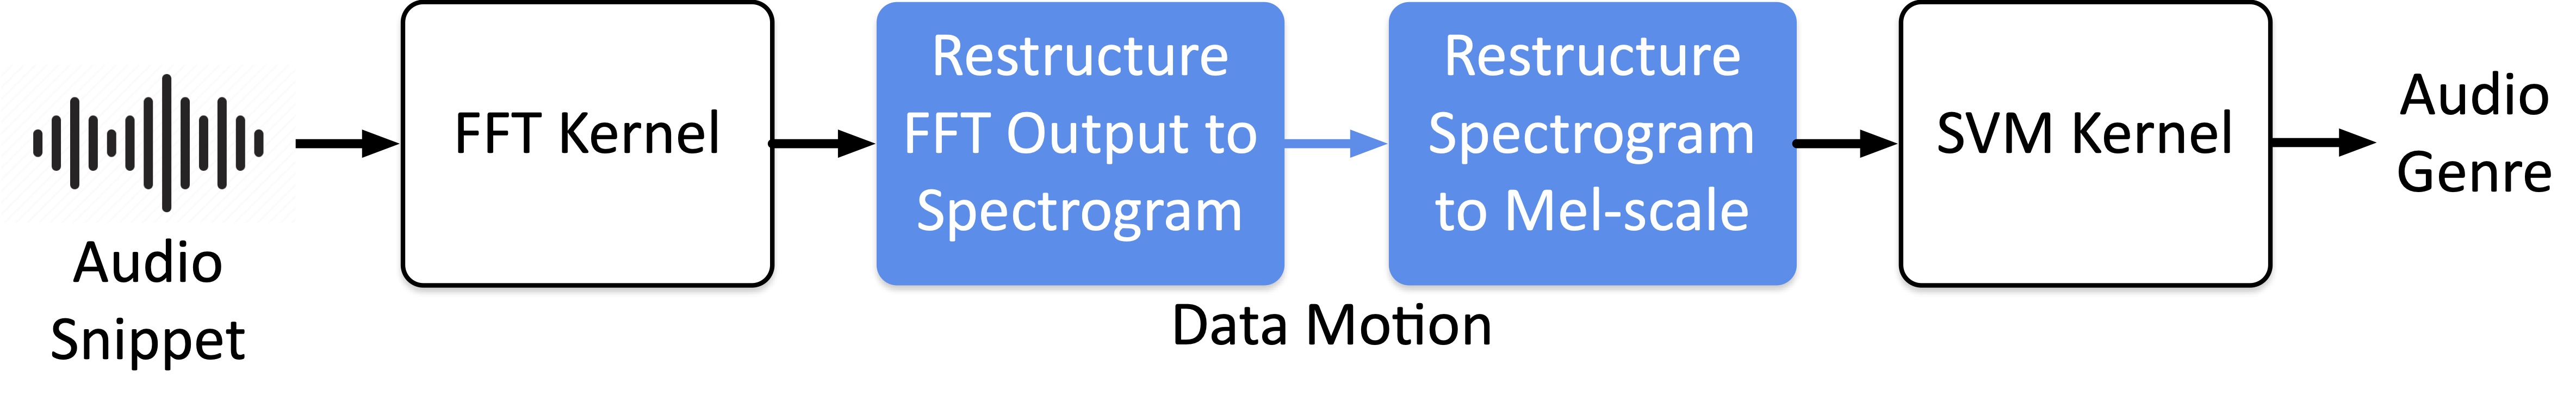
\includegraphics[width=\columnwidth]{figure/fianchetto/motivation_example_a_camera_ready.pdf}
    %\caption{Runtime breakdown when running applications on CPU or multiple accelerator setup that uses CPU for data motion.}
    \caption{}
    \label{fig:motivation:example-a}
    \end{subfigure}
    %
    \begin{subfigure}[b]{\columnwidth}
    \centering{
    \vspace{2ex}
    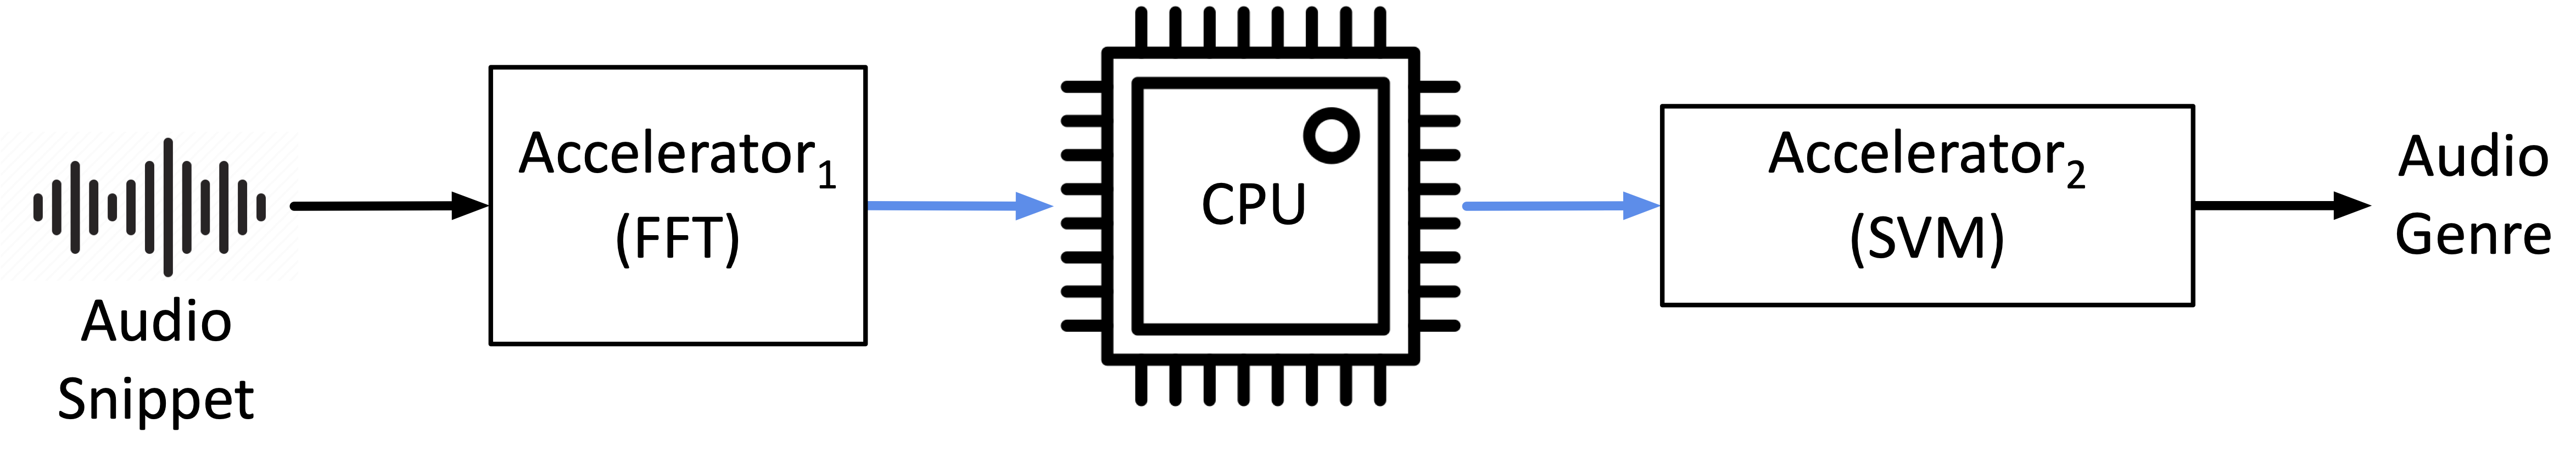
\includegraphics[width=\columnwidth]{figure/fianchetto/motivation_example_b_camera_ready.pdf}
    %\caption{Multi-acceleration performance improvement and scalability are constrained by data motion overhead.}
    \caption{}
    \label{fig:motivation:example-b}
    }
    \end{subfigure}
    %
    \begin{subfigure}[b]{\columnwidth}
    \centering{
    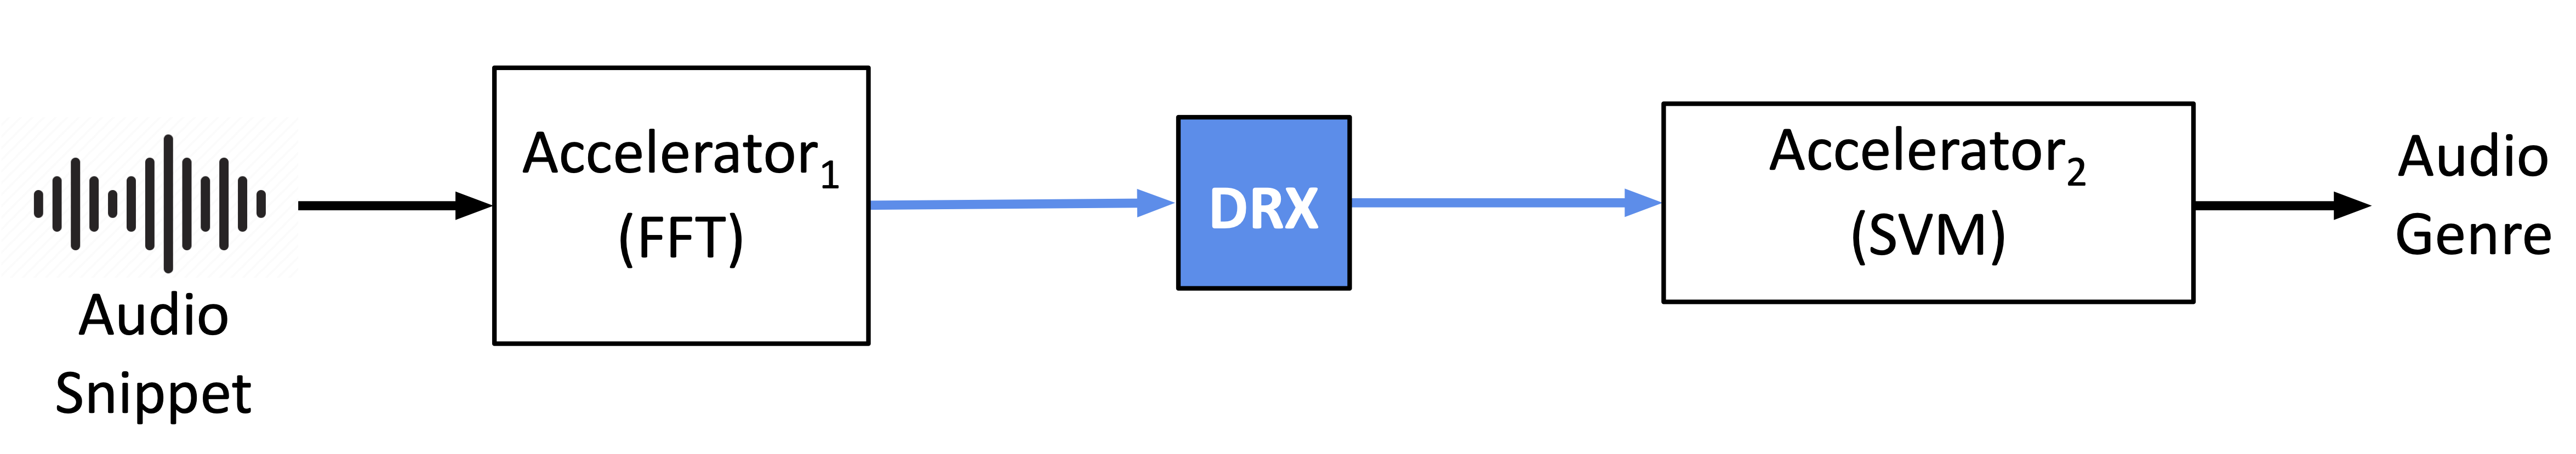
\includegraphics[width=\columnwidth]{figure/fianchetto/motivation_example_c_camera_ready.pdf}
    %\caption{Multi-acceleration performance improvement and scalability are constrained by data motion overhead.}
    \caption{}
    \label{fig:motivation:example-c}
    }
    \end{subfigure}
    % \includegraphics[width=\columnwidth]{ASPLOS23/figures-resubmit/motivation_example_camera_ready.pdf }
    \caption{ 
    (a) Data motion stands between two application kernels, i.e., Fast Fourier Transform and Support Vector Machine, of an end-to-end application.  
    %
    (b) Data motion is on CPU and application kernels are on their corresponding accelerators 
    %
    (c) For \dmx, data motion is accelerated on \drx and application kernels are on their corresponding accelerators.
    }
    \label{fig:motiv-ex}
    \vspace{-3ex}
\end{figure}

\subsection{Data Restructuring Operations}
\label{sec:motivation:operations}


In this work we use five end-to-end applications that span multiple domains~\cite{acc-yolov3:iscas:2020, urbansound-dataset:mm:2014, rldbs:ijcai:2020, microsoft-presidio,doppiodb:fpl:2017,chiosa:pvldb:2022} to quantify the inefficiencies of cross-domain acceleration in current multi-accelerator systems. Each of them has different domain-specific kernels and data restructuring requirements between the kernels. 
%
Specifically, \bench{Video Surveillance} decodes input video streams into video frames and passes them to an object detection kernel~\cite{yolov3}.
%    
\bench{Brain Stimulation} receives electromagnetic signal input generated from a brain simulation model, processes it with FFT and data restructuring operations before outputs the data to reinforcement learning kernel~\cite{rldbs:ijcai:2020}.
%   
\bench{Personal Information Redaction} decrypts privacy-sensitive text and uses a regular expression kernel to detect personally identifiable information and redact them from the text with blanks~\cite{microsoft-presidio}.
%    
\bench{Database Hash Join} decompresses database tables and hash joins the tables~\cite{doppiodb:fpl:2017,chiosa:pvldb:2022}.   

Figure~\ref{fig:motiv-ex}(a) illustrates the end-to-end application pipeline of the \bench{Sound Detection} application. %, which receives an audio snippet and detects its genre. 
%
As shown, \bench{Sound Detection} is composed of two domain-specific kernels:
%
(1) FFT kernel running short-time Fourier transformation for the input audio snippet, and
%
(2) support vector machine kernel to decide the genre of the audio snippet.
%
An intermediate \textit{data motion} step is required for restructuring the output of the FFT kernel to the input format of the support vector machine kernel while copying the data from the output buffer to the input buffer. 
%
In this example, data restructuring requires generating a spectrogram from the output of FFT kernels and applying mel scale transformation to the spectrogram. 
%
The mel scale transformation maps the spectrogram into mel-frequency bins which are closer to the human-perceivable scale.
%

%\malian{@Shu-Ting - add a few sentences explaining Table.\ref{table:data-trans-ops}}\stingw{Done}
%
%Table~\ref{table:data-trans-ops} presents five end-to-end applications~\cite{acc-yolov3:iscas:2020, urbansound-dataset:mm:2014, rldbs:ijcai:2020, microsoft-presidio,doppiodb:fpl:2017,chiosa:pvldb:2022} including \bench{Sound Detection}. Each of them has different kernels and data restructuring operations between the kernels.


%\begin{figure}[h]
\begin{subfigure}[b]{\columnwidth}
\includegraphics[width=\columnwidth]{ASPLOS23/figures-resubmit/motivation-scaling-breakdown.pdf}
%\caption{Runtime breakdown when running applications on CPU or multiple accelerator setup that uses CPU for data motion.}
\caption{}
\label{fig:motivation:bar:breakdown}
\end{subfigure}
%

\begin{subfigure}[b]{\columnwidth}
\centering{
\includegraphics[width=0.65\columnwidth]{ASPLOS23/figures-resubmit/motivation-multiaxl-constraint.pdf}
%\caption{Multi-acceleration performance improvement and scalability are constrained by data motion overhead.}
\caption{}
\vspace{-2pt}
\label{fig:motivation:bar:multiaxl}
}
\end{subfigure}
\caption{(a) Runtime breakdown when running applications on CPU or multiple accelerator setup that uses CPU for data motion. (b) Multi-acceleration speedup and scalability are constrained by data motion overhead.}
\label{fig:motivation:bar}
\end{figure}
\begin{figure}[ht!]
    \begin{subfigure}[b]{0.9\columnwidth}
    \includegraphics[width=\columnwidth]{figure/fianchetto/motivation-multiaxl-breakdown.pdf}
    %\caption{Runtime breakdown when running applications on CPU or multiple accelerator setup that uses CPU for data motion.}
    \caption{}
    \label{fig:motivation:bar:breakdown}
    \end{subfigure}
    %
    
    \begin{subfigure}[b]{0.9\columnwidth}
    \centering{
    \includegraphics[width=0.65\columnwidth]{figure/fianchetto/motivation-multiaxl-constraint.pdf}
    %\caption{Multi-acceleration performance improvement and scalability are constrained by data motion overhead.}
    \caption{}
    \vspace{-2pt}
    \label{fig:motivation:bar:multiaxl}
    }
    \end{subfigure}
    \caption{(a) Runtime breakdown when running applications on CPU or multiple accelerator setup that uses CPU for data motion. (b) Multi-acceleration speedup and scalability are constrained by data motion overhead.}
    \label{fig:motivation:bar}
\end{figure}


\subsection{Data Motion Overheads}
%
%\TODO{explain we use geomean valus acorss 5 apps but not individual apps}
Figure~\ref{fig:motivation:bar}(a) shows the geometric mean of the runtime breakdown for the five %Sound Detection application as well as four other 
applications explained in Sec.\ref{sec:motivation:operations}. We show the results for co-running up to 15 applications on the server while data restructuring is performed on the CPU. \emph{All-CPU} configuration runs application kernels on the CPU while \emph{Multi-Axl} runs the application kernels on the DSAs. Because each application consists of 2 domain-specific kernels, 15 application setup runs on 30 DSAs.
%under two scenarios: the application runs entirely on the CPU (All-CPU setup shown in Fig.\ref{fig:motivation:bar:cpu}) and the application kernels run on accelerators with PCIe interface but Data Motion runs on the CPU (Multi-Accelerator setup shown in Fig.\ref{fig:motivation:bar:accel}). Fig.\ref{fig:motiv-ex}-(b) illustrates the Multi-Accelerator setup. The numbers on the X-axis show the number of concurrent applications running on the systems. We isolate the cores that run application kernels in the All-CPU setup and dedicate 16 cores to Data Motion for both All-CPU and Multi-Accelerator setups. 
%\malian{@Shu-Ting explain the setup in detail. What part of the application is accelerate etc. What is 1 kernel , 5 kernel ... shown in the figures}
%
As Figure~\ref{fig:motivation:bar}(a) shows, in the \emph{All-CPU} setup, the execution of domain-specific kernels accounts for up to 78.5\% and on average 49.1\% of the total runtime.
%
However, the \emph{Multi-Axl} setup reduces the runtime of domain-specific kernels, but at the same time amplifies the ratio of data motion within the end-to-end runtime.
%\malian{ppl will ask what about a middle ground of using a GPU and map both kernels to run on a single GPU (review-E)?}
%
The ratios range from 71.3\% to 97.1\%, showing that data motion becomes the performance bottleneck under multi-acceleration.
%
%The efficiency of data motion determines the end-to-end performance of multi-accelerated applications. This motivates the necessity of data motion acceleration. 
%Therefore, data motion acceleration becomes a timely challenge to unleash the full benefits of multi-acceleration.
%

Another important observation from Figure~\ref{fig:motivation:bar} is the poor scalability of current multi-accelerator systems when concurrently running applications on multiple accelerators. 
%1. 1-> 5, data movement bottleneck on the CPU -> accelerator link.
From a single application to 5 applications, data movement emerges as a bottleneck. The limited PCIe bandwidth of CPUs creates a bottleneck for data moving in and out of CPU for data restructuring operations as they cannot directly connect all accelerators concurrently. %\krishnan{to themselves or concurrently?}.
%2. 5->10 and 15, data restructuring on CPU accounts for more portion of end-to-end runtime.
As the number of applications grows further to 10 and 15 applications, the CPU demonstrates its incapability to keep up with the increased concurrency of data restructuring operations though using 16 Xeon cores. % out of 20 physical cores on a Xeon server processor.
%
Such a bottleneck in data movement and data restructuring stifles the end-to-end speedup achieved by multi-acceleration at scale. As shown in Figure~\ref{fig:motivation:bar}(b), accelerating application kernel while relying on the CPU for data restructuring achieves 1.4$\times$ and 1.1$\times$ end-to-end speed up for 1 and 10 applications, while the geometric mean of per DSA speedup is 6.5$\times$. %\TODO{write about limited speedup shown in Figure~\ref{fig:motivation:limited-speedup}}
%
% The speedup of multi-acceleration with ideal data motion acceleration can be projected by Amdahl's law.
% %
% As shown in Figure~\ref{fig:motivation:ideal-speedup}, an ideal data motion acceleration offers 5.1x speedup for multi-acceleration and an overall 23.9x speedup compared to All-CPU baseline.
%

The above results demonstrate the untapped potential of multi-acceleration with ideally accelerated data motion.
%
This significant performance difference between end-to-end and per-kernel speed-up stems from the following \textbf{I}nsights:
%
\textbf{(I1)} Using specialized accelerators reduces the runtime of kernels significantly, shifting Amdahl's bottleneck towards data motion.
%
\textbf{(I2)} Host CPU engagement imposes inevitable data communication with accelerators, adding the cost of data movement on top of data restructuring.
%
\textbf{(I3)} Heterogeneity in the architecture of both accelerators and CPU demands additional data type conversions and layout transformation on top of discussed data restructuring, further amplifying the cost of data motion.
%
Heeding these insights, this work makes a case for accelerating the data motion.
%
%This paper sets out to seize this rather overlooked opportunity and introduce the new concept of data motion acceleration through careful design of system layer and hardware specialization without changing the way the current multi-accelerator systems are being programmed.
%

\section{\dmx: Accelerating the Data Motion}
\label{sec:dmx}
% \begin{comment}
% \stingw{dump notes here:
% 1. control plane is still on CPU with polling → we don’t include the software overhead of the data movement
% 2. Assume a userspace/kernel bypassing poll mode driver
% 3. we should include (1) the overhead of first loading data onto the accelerator (DMA time)
% (2) last load data back to main memory (DMA time), (3) control overhead of polling (See Pond paper for exact latency number)
% }
% \end{comment}

Multi-acceleration in Figure~\ref{fig:motiv-ex}(b) represents the current system design using CPU for data motion. This design requires data to move through the CPU for restructuring the output of one accelerator before the data can be used by the next accelerator. 
%
In this paper, we propose Data Motion Acceleration as illustrated in Figure~\ref{fig:motiv-ex}(c) to facilitate data motion between heterogeneous accelerators. %\dmx avoids the unnecessary data movement between CPU and accelerator and accelerates the non-trivial operations of data restructuring.
%
\dmx accelerates data restructuring and bypasses CPU for data movement between accelerators via integrating the purposefully-built Data Restructuring Accelerator (\drx) into the system.
%
%achieves this goal by accelerating the execution of data restructuring, and offloading the data movement from CPU when multiple accelerators communicate with \hanyang{add software} and a purpose-built Data Restructuring Accelerator (DRX).}
%
%Accelerating the data restructuring motivates the design of a Data Restructuring Accelerator (DRX), purpose-built for executing data restructuring operations. 
%Fig.~\ref{fig:motiv-ex}-(c) illustrates a two accelerator setup with \dmx.  %The location and integration of the data motion accelerator with other accelerators directly impact the overall data movement.
%
Realizing \dmx requires synergistic design considerations at the following levels: % of (1) \drx placement, (2) system integration and programmability, (3) specialized hardware design:
%
%\stingw{structure is okay, namding of drx and dmx might change later, use macro}
\begin{itemize}
\item \textbf{\drx Placement. }
%\stingw{make sure this is consistent with the updated DRX placement in Sec.~\ref{sec:design}}
%
An important design decision in \dmx is the location of the \drx. 
%
The placement of DRX impacts the data movement and the overall system design.
%
We consider three different placements for \drx: integration on the CPU, standalone PCIe-attached card, and per accelerator bump-in-the-wire placement. 
%
% The placement of \drx impacts the data movement and the overall system stack design.

\item \textbf{Specialized Hardware Acceleration.}
%
We need to design \drx to be programmable and support a range of data restructuring operations. 
%%As Figure~\ref{fig:motivation:bar:accel} 
As Figure~\ref{fig:motivation:bar}(a) shows, data restructuring accounts for 57.7\%$\sim$73.2\% of end-to-end runtime, therefore efficient execution of data restructuring is critical for multi-acceleration.  

\item \textbf{System Integration and Programmability.}
%
%\TODO{first explain how current multi-acceleration works, and then we take it from there, with minimal changes to the way we program it. it needs to be usable otherwise it's useless}
%\stingw{make sure this is consistent with the updated system design especially the programming model}
%
To minimize data movement, the CPU should be removed from the data path of accelerator-to-accelerator communication. 
%
However, the control plane should run on the CPU, otherwise, it requires a completely new programming interface that stifles interoperability of \dmx across arbitrary accelerators.
%
In Sec.\ref{sec:system} we explain the current programming interface of multi-accelerator systems and how \dmx only offloads the data plane to the hardware without changing the current control plane.  

\end{itemize}


In Sec.\ref{sec:placement} we explore various placements for \drx and show that tight integration of \drx and accelerators in a bump-in-the-wire fashion minimizes the data movement and delivers the best performance and energy efficiency at scale. 
%
%
Next, we demystify the data restructuring operations in Sec.\ref{sec:accelerator} and introduce a programmable accelerator specialized for the data restructuring domain. 
%
Lastly in Sec.\ref{sec:system}, we discuss the runtime and kernel drivers that coordinate the offload of data restructuring operations to bump-in-the-wire \drx while still running the control plane on the CPU. 

\section{\drx Placement}
\label{sec:placement}

The key design considerations in designing \dmx are the placement of \drx and interconnection between \drx, accelerator, and CPU in the system.
%
Since \dmx is to enable interoperability between accelerators designed by different vendors, \drx's interconnect should be standard and well adopted.
%The interconnect needs to have been well-adopted for most of the devices and accelerator cards.
%
As such, the current incarnation of \dmx considers PCIe as the standard interconnect to connect accelerators to CPU and \drx. 
%
PCIe is a well-established standard of interconnect and serves as the basis for future interconnects such as CXL~\cite{cxl-3-0-spec}.  
% battleground-tested technology and future interconnects such as CXL are built atop PCIe physical layer~\cite{cxl-3-0-spec}. \hanyang{Not clear, you should say something like PCIe is industry-standard (possible one citation) and future prove (the CXL example you provided)}
%

The placement of \drx ideally should (1) scale with the capacity of associated accelerators, (2) avoid being the bandwidth bottleneck when accelerators transfer/receive data from it, and (3) minimize data movement as data movement is the main performance and energy bottleneck in today and future system~\cite{horowitz:isscc:2014}.

\begin{figure}[ht!]
    \centering
    \includegraphics[width=0.90\columnwidth]{figure/fianchetto/drx_cpu_config_camera_ready.pdf}
    \caption{Integrated \drx.}
    \label{fig:integrated-drx}
\end{figure}

%\noindent \textbf{\drx integrated with CPU.}
\noindent \textbf{Integrated \drx into CPU.}
This configuration considers integrating \drx with the CPU as illustrated in Figure~\ref{fig:integrated-drx}. 
%Figure~\ref{fig:integrated-drx}. 
%
The integrated accelerators become more common recently as Intel Sapphire Rapids, IBM z15, POWER9, and Telum offer them in their CPU products~\cite{intel-sapphire-rapids:hotchips:2021,ibm-compression-accelerator:isca:2020,ibm-telum-processor:isca:2022}.
%
Integrated accelerators are efficient in performing computation on the data that is on the CPU chip. However, integrated accelerators are going to eat up the already limited CPU power budget~\cite{dark_silicon_isca2011,dark_silicon:babak}. 
%suffer from the limited power budget as CPUs are often operating at tight power and thermal constraints~\cite{dark_silicon_isca2011,dark_silicon:babak}. \malian{SAY: accelerators are going to eat up the CPU power budget.}
%These accelerators are convenient to use as they are integrated into the CPU but this also limits the amount of power it can consume. The accelerator when running on IBM POWER 9 draws 33 Watts active power. 
%
Such power and thermal constraints limit the performance of integrated accelerators on the CPU.
%
% For example, 
% % the compression unit in IBM POWER 9 is limited to 33 Watts of active power~\cite{ibm-compression-accelerator:isca:2020} and 
% Intel Sapphire Rapids can only activate up to a fixed amount of accelerators~\cite{supermicro-sapphire-rapids}. \stingw{for supermicro servers, they can activate up to 12 from 4 types of accelerators, QAT, DLB, DSA, and IAA.} \krishnan{see comments in my email}
%

\dmx considers a fixed power budget 
%\krishnan{can't we just say -- We consider a fixed power budget -- instead of specifing it to be 34 Watts?} 
for an integrated accelerator and design an Integrated \drx to operate within this power limit~\cite{supermicro-sapphire-rapids, ibm-compression-accelerator:isca:2020}.  
%
% 34 Watts derived from the active power when IBM compression accelerator running max workload on POWER9 CPU~\cite{ibm-compression-accelerator:isca:2020}.
%\stingw{34 Watts derived from the active power when IBM compression accelerator running max workload on POWER9 CPU. }
%
%For integrated \drx, only a fixed amount of \drx hardware based on the exact power of \drx can be placed on the CPU.   
%
This fixed power budget limits the performance of \drx.
%
As we will show in Sec.\ref{sec:results}, Integrated \drx becomes the performance bottleneck when scaling the number of accelerators to more than 8.
%    
Although integrating \drx %as a separated die 
using die-to-die interconnects like UCIe could alleviate the affect, integrated \drx still become the performance bottleneck with excessive data movement~\cite{amd-chiplet:isca:2021, odsa-bow-spec, ucie-spec}.
%This fixed amount prevents \systemName to further scale the compute from \drx to match up with the data restructuring demand from accelerators.
%
Moreover, Integrated \drx has the same data movement as the baseline CPU without \drx. Such design requires all accelerators to send their data to the CPU which makes the PCIe link connecting the CPU to the accelerators the bandwidth bottleneck when multiple accelerators use \drx at the same time. Such data movement is also the main source of system energy consumption. %PCIe switches creates bandwidth oversubscription that force accelerators to share their bandwidth to move data in and out of \drx on the CPU.
%Moreover, \drx integrated with CPU imposes a bandwidth bottleneck when PCIe switches are introduced to accommodate the growing number of accelerators. PCIe switches creates bandwidth oversubscription that force accelerators to share their bandwidth to move data in and out of \drx on the CPU.

\begin{figure}[ht!]
    \centering
    \includegraphics[width=0.90\columnwidth]{figure/fianchetto/drx_pcie_config_camera_ready.pdf}
    \caption{Standalone \drx. Number of \drx units in Standalone placement is configurable, and the illustration represents just one possible configuration.}
    \label{fig:standalone-drx}
\end{figure}

\noindent\textbf{Standalone \drx as a PCIe card.}
This configuration considers implementing \drx as a standalone PCIe card that is installed just like any other accelerator on a PCIe slot. 
%aggregating a certain units of \drx hardware.  
%
%The advantage of the standalone \drx is the higher power budget of a PCIe card compared with an integrated \drx. 
%
Without using an external power supply cable, the performance of a single Standalone \drx PCIe card is limited by the PCIe power supply standard, which is 25 Watts.
%
Nevertheless, as illustrated in Figure~\ref{fig:standalone-drx}, installing multiple Standalone \drx cards can scale \drx performance with the number of accelerators. 
%resolves the power limit imposed by CPU integration and further the scale of \drx to match up with the number of accelerators.  
%
However, this Standalone \drx still incurs bandwidth oversubscription as the PCIe link to a shared, Standalone \drx card can become the bottleneck. 
%However, this Standalone \drx still incurs bandwidth oversubscription as accelerator accessing a piece of shared hardware below a PCIe switch.
%

Compared to Integrated \drx, a Standalone \drx has the potential to reduce the data movement if \dmx implements a point-to-point PCIe connection between \drx card and accelerator cards. This way, a Standalone \drx can localize the communication under the PCIe switch to which other accelerator cards are installed. 
%\hanyang{So is it implemented this way in the experimental setup? If not the speedup/energy reduction should not be scaling with the application count in the standalone configuration, if so, you shouldn't say it has the potential, just say it does}
%\stingw{something more exactly about how its bandwidth oversubscription is different from CPU's case.}
%\stingw{we still have BITW but we'll have a internal PCIe switch like Samsung SmartSSD shown in their documentation.~\cite{samsung-smartSSD:documentation:2020}}

\begin{figure}[ht!]
    \centering
    \includegraphics[width=0.90\columnwidth]{figure/fianchetto/drx_pcie_switch_config_camera_ready.pdf}
    \caption{PCIe-Integrated \drx.} 
    \label{fig:drx-config-on-pcie-switch}
\end{figure}

\noindent\textbf{PCIe-Integrated \drx.}
This configuration integrates \drx onto a PCIe switch (Shown in Figure~\ref{fig:drx-config-on-pcie-switch}).
%
%Compared to a Standalone \drx, A PCIe-Integrated \drx saves a round-trip between the source \drx and the source PCIe switch and a pass through the destination PCIe switch.  
Compared to a Standalone \drx, A PCIe-Integrated \drx saves a round-trip between \drx and the PCIe switch.  
%
However, PCIe-Integrated \drx requires \drx to operate at the aggregated rate of all downstream PCIe ports, which adds considerable hardware complexity. 
%
Also, computation on switches only permits limited memory usage and a limited number of instructions per packet~\cite{rmt:sigcomm:2013,drmt:sigcomm:2017,in-network-compute:hotnets:2017,in-network-compute:eurosys:2019}. 
%
This configuration requires significant engineering effort to redesign the PCIe hardware and related software stack. 

\begin{figure}[ht!]
    \centering
    \includegraphics[width=0.90\columnwidth]{figure/fianchetto/drx_acc_config_camera_ready.pdf}
    \caption{Bump-in-the-Wire \drx.
    }
    \label{fig:drx-config-acc}
\end{figure}

\noindent\textbf{Bump-in-the-Wire \drx.}
Lastly, we introduce a Bump-in-the-Wire \drx configuration 
inspired by Catapult~\cite{catapult:isca:2014} that connects an exclusive \drx to each accelerator (Figure~\ref{fig:drx-config-acc}).

Bump-in-the-Wire configuration avoids overprovisioning of PCIe links and \drx resources for a multi-accelerator system and enables \dmx to scale with the hardware resources compared with the other configurations.
%
More importantly, Bump-in-the-Wire \drx placement reduces the data movement to a minimum when accelerators communicate with each other.
%
%Accelerators and their \drx can be tightly integrated on the same chip with unified memory to avoid any data movement between them. 
%
Coupled with a programmable \drx that enables offloading of any data restructuring operation (c.f., Sec.\ref{sec:accelerator}), Bump-in-the-Wire \drx serves as an option to build future scalable multi-accelerator systems.


\section{Data Restructuring Accelerator (\drx) Design}
\label{sec:accelerator}

As discussed in Sec.\ref{sec:motivation}, the CPU is not an optimal place to perform data restructuring operations. 
In this section, we first analyze different data restructuring operations by profiling their execution on the CPU. This analysis guides us in devising a programmable accelerator specialized for the data restructuring domain. Refer to Sec.\ref{sec:method} for more information on the experimental setup. %Then we use the insights to devise a programmable accelerator specialized for the data restructuring domain. 

\begin{figure}[ht!]
    \centering    
    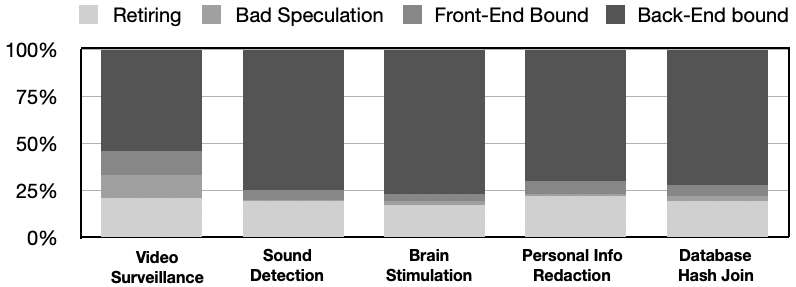
\includegraphics[width=0.9\columnwidth]{figure/fianchetto/profiling_vtune.pdf}
    \caption{Top-down breakdown of stall cycles for data restructuring operations.}
    \label{fig:topdown}
\end{figure}

\subsection{Data Restructuring Characterization}
%We profiled the five representative data restructuring operations explained in Sec.\ref{sec:motivation:operations}. 
%
%The data restructuring operations are implemented using PyTorch which uses Intel oneAPI Math Kernel Library (MKL). MKL transparently vectorizes data restructuring operations when running on a CPU by using AVX-256, AVX-512, or newer SIMD instructions. 
%
%We use Intel Vtune Profiler~\cite{vtune} to profile the operations and list several observations. These observations guide our design of \drx. Refer to Sec.\ref{sec:method} for more information on the experimental setup. 
Figure~\ref{fig:topdown} shows the top-down~\cite{top-down:ispass:2014} breakdown of stall cycles for data restructuring operations. 
%\malian{cite top down paper: https://ieeexplore.ieee.org/document/6844459} 
%
We characterize data restructuring operations with the top-down analysis of Intel VTune~\cite{intel-vtune} on an Intel Xeon Gold 6242R processor. 
%
The processor has the same microarchitecture as our testbed setup on AWS (See Sec.\ref{sec:method} for details).
%
%As shown, the operations are either waiting for the backend or retiring. 
Across different data restructuring operations, we see at most 12.5\% Bad Speculation Bound and 14\% Front-End Bound cycles. A deeper analysis of \textit{Video Surveillance} reveals that this distinct behavior is linked to a higher number of branch instructions, resulting in a relatively larger number of cycles spent on branch re-steer and uOp cache switches. On the other hand, the Back-End Bound cycles range from 53\% to up to 77.6\% of total cycles. The culprit for Back-End Bound cycles is both the unavailability of functional units and misses in the data cache. 23.2\% of Back-End Bound cycles are Core-Bound and 46\% are Memory-Bound. %Because the data restructuring operations have plenty of data level parallelism, the Top-Down breakdown suggests that they are contending for functional units and waiting for memory. 

The profiling shows that data restructuring operations have low L1I cache Misses Per Kilo Instructions (MPKI). The average L1I MPKI for data restructuring is 2.3. As a reference, our measurements for online services from CloudSuite~\cite{noauthor_cloudsuite_nodate} report an average of 7.8 L1I MPKI. 
%0.1$\sim$4.1 
%with an average while MPKI of SPEC 2017\cite{speccpu2017} is 0.1$\sim$11.6~\cite{panda_wait_2018}. 
Such low L1I MPKI suggests a small instruction working set for data restructuring operations that fit inside the L1I cache of the core. 

%\noindent{\textit{Observation3: data restructuring operations have plenty of data-level parallelism.}}

The profiling results show that all data restructuring operations have a high degree of vector unit utilization. The data restructuring kernels use 100\% of available vector unit capacity which is 256 bits wide AVX-256 on our servers. 
%However, we observe that the data restructuring kernels can only utilize 50\% of the available vector unit capacity. This is because the %vector operations are 256 bits wide while the Xeon CPU implements 512-bit wide vectors. 
We also observe a high number of ephemeral threads that are spawned by the Intel Math Kernel Library while restructuring the data. The number of threads that are spawned while running the data restructuring operations is between 130 to 140. These threads operate on the data in parallel and illustrate the high data-level parallelism and inefficiency of CPUs in executing the data restructuring operations.

%\vspace{-2ex}
\subsection{\drx Hardware Architecture}
We use the above insights to design a programmable \drx that specializes in the data restructuring domain.
%
The main observations driving \drx design are the abundance of data-level parallelism, streaming access pattern, and non-trivial operations of data restructuring. Figure~\ref{fig:drx-acc-arch} overviews the architecture of \drx hardware.
%

\drx uses a decoupled access-execute architecture that consists of a programmable front-end specialized for walking over multi-dimensional data structures, and a configurable number of interleaved vector processing units dubbed Restructuring Engine (RE) in the same pipeline. 
%
It also includes a Transposition Engine for data transposition operations and a programmable Off-chip Data Access Engine for off-chip load/store which also houses a DMA engine that initiates data movement with other accelerators.  %128-lane 256-bit vector processing unit dubbed Restructuring Engine (RE) in the same pipeline. It also includes a Data Transposition Engine to ensure full coverage of data transposition scenarios. 
%
For evaluation, we configure the \drx to contain 128 lanes of RE, a 64KB instruction cache, a 64KB data scratchpad, and 8GB of DDR4 DRAM.  %\malian{should we make it 8GB considering that we need more memory to map buffer for DRX-DRX communication?}. 
A DDR4 3200 memory channel sustains $\sim$25GBps, therefore \drx implements a single DDR4 channel to match the bandwidth of an x8 PCIe Gen 4 link.%\malian{for the evaluation we use these. Seperate the general design and then one for specification.}
%
% When issuing instructions to \drx REs, the Instruction Repeater in the front-end tracks the loop iteration and calculates the scratchpad addresses based on the configuration stored in Strided Scratchpad Address Calculation, eliminating the need for vector register files and issuing excessive numbers of memory instructions.
% %
% Instead, the data is fetched from the interleaved scratchpads in the REs based on pre-computed addresses by the front-end. 
% %
% A programmable Off-chip Data Access Engine connects these scratchpads for DRAM load/store, the Off-chip Data Access Engine also houses the DMA engine that initiates data movement with other accelerators. 
% %

\noindent \textbf{\drx ISA. }
The DRX ISA and hardware architecture are optimized based on the observation that data restructuring workloads consist of known-shape, pre-located multidimensional arrays. Such arrays can be indexed using a set of loops. As shown in Figure~\ref{fig:drx-acc-isa}, the DRX ISA includes specialized loop, compute, off-chip memory access, and synchronization instructions for vector operations while preserving the option for scalar operations, enabling serial tasks like pointer dereferencing.

%DRX ISA and hardware architecture are optimized based on the observation that data restructuring workloads consist of known-shape, pre-located multidimensional arrays, and such multidimensional arrays can be indexed with a set of loops.
%
%As such, DRX ISA consists of loop, compute, off-chip memory, and synchronization instructions that are specialized for vector operation while still preserving the option to operate on scalar, which enables serial operations such as pointer de-reference.
%
The DRX ISA significantly departs from traditional SIMD semantics, offering optimizations for memory, loops, and data packing. 
%
For memory optimization, DRX employs software-managed on-chip scratchpads instead of vector register files and the conventional cache hierarchy found in common SIMD ISAs. 
%
Memory instructions configure the Off-chip Data Access Engine to fetch data directly from DRAM to the on-chip scratchpads. 
%
For loop optimization, DRX utilizes hardware loops within an Instruction Repeater unit to reduce branch instruction overhead. 
%
Loop instructions configure the Instruction Repeater based on the dimensions of the kernel's multidimensional arrays. 
%
For data packing optimization, the DRX compiler partitions the kernel's multidimensional arrays across the REs, eliminating the need for pack/unpack instructions.

%DRX ISA is a significant departure from the traditional SIMD semantics and offers optimization for memory, loop, and data packing. For memory optimization, DRX uses software-managed on-chip scratchpads instead of vector register files and conventional cache hierarchy in common SIMD ISA. Memory instruction configures the Data Access Engine to fetch data from DRAM directly to on-chip scratchpads. For loop optimization, DRX uses hardware loops within Loop Repeater to eliminate branch instruction overhead. Loop instructions configure the Instruction Repeater based on the dimensions of kernel multidimensional arrays. For data packing optimization, the DRX compiler partitions the kernel multidimensional arrays across the REs to eliminate the need for pack/unpack instructions. 

During the vector execution, loop instructions first configure the Off-chip Data Access Engine and Strided Scratchpad Address Calculator with sets of <Base, Stride, Iteration> configurations that correspond to the input/output loop dimensions and data location. 
%
After the Off-chip Data Access Engine loads the data to scratchpad banks, compute instruction is issued with scratchpad addresses calculated by the Instruction Repeater by traversing the dimensions of multidimensional arrays based on the configurations in the Strided Scratchpad Address Calculator. 
%
This data access scheme significantly reduces memory and address calculation overhead and is applied to all operations on multidimensional arrays such as data transformation, memory access, and compute operations. 
%
Finally, synchronization instructions are issued at the start and the end of the instruction stream to ensure proper program order. For scalar execution, \drx turns off all but one REs and operates as a scalar in-order CPU. 


\begin{figure}[ht!]
    \centering
    \includegraphics[width=0.9\columnwidth]{figure/fianchetto/drx-acc-arch.pdf}
    \caption{DRX Hardware Architecture.
    }
    \label{fig:drx-acc-arch}
    \vspace{-2ex}
\end{figure}

\begin{figure}[ht!] 
    \centering
    \includegraphics[width=0.9\columnwidth]{figure/fianchetto/drx-acc-isa.pdf}
    \caption{DRX instruction types.}
    \label{fig:drx-acc-isa}
\end{figure}

\noindent \textbf{\drx compiler.}
%We design a compiler that can
Inspired from prior works~\cite{tvm:osdi18, autotvm:2018} in other domains, \drx compiler compiles high-level data restructuring kernels into \drx instructions based on the DRX ISA.
%
% \drx compiler compiles high-level high-level data restructuring operations into \drx instructions based on the ISA. 
%
The \drx compiler takes two inputs: a high-level representation of the data restructuring kernel and an architecture configuration file that defines the \drx hardware configurations such as the number of REs and on-chip scratchpad size.
 %
The compiler first maps the data restructuring kernel to the intermediate representation of the kernel operations.
 %
 It then optimizes tiling and relaxes dependency on the intermediate representation based on the hardware configuration and the dimension of multidimensional arrays. 
 %
 Finally, it generates instructions based on \drx ISA from the optimized intermediate representation.
 %
 Figure~\ref{fig:drx-acc-kernel} shows a sample of the DRX kernel.
 %
 %We will open-source the compiler and DRX Verilog implementation.

 \section{System Integration and Programmability}
\label{sec:system}

In this section we discuss the system integration and programmability of \dmx with Bump-in-the-Wire DRX placement. The system integration of other DRX placements share many similarities with Bump-in-the-Wire DRX.

\noindent \textbf{Programming model.}
\dmx implements an OpenCL-style programming model that has a host program on the CPU and kernels on accelerators or \drx. 
%
Application kernels are executed on accelerators while data restructuring kernels are executed on \drx.
%
Because \dmx runs the control plane on the CPU, it does not compromise the programmer's productivity and does not incur any additional accelerator orchestration overhead compared to the baseline multi-acceleration system. % incurs the same level of system overhead as the multi-acceleration baseline because both are based on the composition of host program and kernels~\cite{opencl,xilinx-vitis-vivado:2020,oneapi}.
%}

The host program creates an execution context for each instance of the application kernel or data restructuring kernel. The context includes (1) the hardware -- e.g. the accelerator or \drx -- involved in the applications, (2) application or data restructuring kernels, and (3) a per accelerator \textit{command queue} that is mapped to the global host address space. The command queue is used for buffering the output of the application kernels and the restructured input of the next application kernel before being transferred to the destination.

The host program uses user-level OpenCL API to create the execution context. 
%
It also uses the API to interact with the accelerators and \drxs through their own \textit{command queue} on each device. 
%
The command queue accepts commands to enqueue kernels for execution, transfer data, or synchronize memory buffers. %\malian{do we talk about all these functions?} \stingw{we need the three of them here. I deleted map/unmap as we don't map memory buffer to user space in our use case.}.
%The command queues accept commands to enqueue kernel and data restructuring program for execution, transfer/synchronize memory buffers, or map/unmap memory buffer in the host memory.
%
The execution of a command can be blocking or non-blocking. 
%
Blocking execution does not return to the host program before the current command completes. 
%
Non-blocking execution, on the other hand, requires a detailed description of the dependency between kernels and data restructuring programs. 
%
For a single command queue, the queued commands are executed in the order they are enqueued.

%\dmx follows OpenCL style programming model. It considers a host connected with one or more accelerators. An application using \systemName implements host program, kernel program running on accelerators, and data restructuring program on DRX.
%
The application kernels execute domain-specific kernels of the end-to-end application on different accelerators. 
The data restructuring kernels perform the required data restructuring operations when two accelerators are communicating. The host program executes the serial portion of the application and runs a daemon to orchestrate the execution of application and data restructuring kernels running on accelerators and \drxs, respectively. 
%A host-side program orchestrates the execution of kernels and data movement, which can be between the CPU and accelerators or between accelerators. 
%
%A kernel program executes the kernel specified by the application.
%
The data restructuring kernels are shipped to \drxs that understand the exact input and output format of each accelerator. The data restructuring kernels are engaged to ensure that properly structured input/output data is moved directly between accelerators and \drx.
% \malian{You need to check how P2P works, explain it, and then define \dmx programming to follow P2P style of programming two accelerators.}

\begin{figure}[t]
    \centering
    \includegraphics[width=\columnwidth]{figure/fianchetto/drx-acc-kernel.pdf}
    \caption{Sample DRX kernel.}
    \label{fig:drx-acc-kernel}
\end{figure}

%\TODO{mention who provides the device driver-> accelerator vendor/developer}
\noindent \textbf{Driver support for \dmx.} 
At a high level, \dmx enumerates both accelerators and \drxs as PCIe devices connected to the CPU.  
%
%\dmx drivers include accelerator driver to initialize and control the accelerator cards, 
%
Each \drx unit has a driver to initialize the command queues, exchange the start and end pointers of the queue to other \drxs at the start, and orchestrate data restructuring operations. 
%
The drivers use GEM~\cite{linux-drm-gem,linux-gem-lwn} for command executions and memory-related operations. \drx driver executes commands and reads/writes/maps operations using ioctl syscall. 
%for device-specific operations.
%
For setting up point-to-point DMA between \drx and accelerators, the drivers use dma-buf API~\cite{dma_buf:kernel:2022}.
%An interconnect driver orchestrates peer-to-peer DMA between \drx and accelerator.
%
The vendor-specific accelerator drivers should support point-to-point DMA in order to work with \dmx.
%The drivers of accelerators are provided by the vendors as they contain device-specific details. 
%\stingw{NAPI-like interrupt handling is here}
By default, we operate accelerators and \drxs in interrupt mode for sending notifications to the CPU. The interrupt handling of the drivers utilizes interrupt coalescing for the bursty arrival of interrupts. 
%
If the arrival rate of interrupts exceeds a certain threshold, the drivers switch to polling. This design is similar to Linux NAPI design~\cite{napi:kernel:2022}.
% \stingw{accelerator driver:}
% It initializes the  

\begin{figure}[t!]
    \centering
    \includegraphics[width=0.9\columnwidth]{figure/fianchetto/data-queue-on-drx.pdf}
    \caption{ 
    %\drx's memory space and RX/TX data queue pairs. \drx uses the data queue as a circular buffer with head and tail pointers. \textit{$RX_{i}$} receives data from other accelerators sending its data to ${Accelerator}_{i}$. \textit{$TX_{i}$} sends restructured data from \drx to ${Accelerator}_{i}$. \drx supports up to a total $n=40$ accelerators in the current design.
    RX/TX data queue pair architecture in Bump-in-the-Wire \drx. \drx uses the data queue as a circular buffer with head and tail pointers. The output of the accelerator that is destined for ${Accelerator}_{i}$ is enqueued in \textit{$RX_{i}$} before being restructured and stored in \textit{$TX_{i}$} for transmission to ${Accelerator}_{i}$. Current \drx implementation supports up to a total $n=40$ accelerators.
    }
    \label{fig:system:data-queue}
\end{figure}

\begin{figure}[t!]
    \centering
    \includegraphics[width=\columnwidth]{figure/fianchetto/p2p_dma_workflow_camera_ready.pdf}
    \caption{Point-to-point DMA workflow involves two accelerators and the sending side \drx. 
    %
    The DMA bypasses the receiving side \drx.
    %
    \dmx supports other communication patterns such as broadcast and multicast among \drxs and between \drxs and accelerators.
    }
    \label{fig:system:p2pdma}
\end{figure}

%\noindent \textbf{\drx driver.}
Although Bump-in-the-Wire \drx is attached to each accelerator, each \drx unit should be able to set up a point-to-point connection with all the other accelerators and \drxs in the system.
%
The memory address space of each \drx is statically partitioned between all the accelerators as well as \drxs in the system to implement two pairs of RX/TX \textit{data queues} per accelerator on each \drx: one pair of queues for direct \drx-accelerator communication and another pair of queues for \drx-\drx communication.
%types of RX/TX \textit{data queues} per accelerator on each \drx: a type of queue pairs for communicating with other accelerators and another type of queue pairs for communicating with other \drxs.}
%a pair of \textit{data queues} per accelerator on each BITW \drx: RX and TX data queues.
%to serve a fixed number of accelerators. 
%

The number of accelerators is determined at PCIe enumeration time when it discovers connected accelerators that need data restructuring. We provision 8GB of memory space for implementing data queues on each \drx. The size of each data queue pair is 100MB. This will enable \dmx to support up to 40 accelerators on a server. 
%The memory address space of each \drx is statically partitioned to serve a fixed number of accelerators. 
%
\drx driver maintains a head and tail pointer for each data queue to keep track of the data that is enqueued for restructuring. 
%
RX and TX data queues on a \drx are shown in Figure~\ref{fig:system:data-queue}.
%
A point-to-point DMA moves data between data queue pairs and accelerator memory. %The memory buffer stored on \drx's memory partition is used for peer-to-peer DMA between accelerators and \drxs. 
%
% Peer-to-peer DMA enables \drx as a BITW to be passed through on the receiving side when no data restructuring operation is needed. 


GEM allocates and frees data buffers opaquely because it is agnostic to the data content in the buffer. %The driver creates memory buffers from the memory allocation of GEM. 
%
The allocated data buffers are referred to by their handle, which is equivalent to a file descriptor. %in user space for applications. 

%\noindent \textbf{Peer-to-peer DMA Among Accelerators and \drxs.}
\begin{table*}[ht!]
    \centering
    \resizebox{\textwidth}{!}{%
    \footnotesize{
    \begin{tabular}{|l|l|l|l|l|l|l|}
\hline
\textcolor{black}{Benchmark} &
  \textcolor{black}{Kernel 1} &
  \textcolor{black}{Kernel 1 Accelerator} &
  \textcolor{black}{Data Restructuring} &
  \textcolor{black}{Kernel 2} &
  \textcolor{black}{Kernel 2 Accelerator} &
  \textcolor{black}{Input Dimension} \\ 
\hline
 \begin{tabular}[c]{@{}l@{}}Video\\ Surveillance~\cite{acc-yolov3:iscas:2020}\end{tabular}&
  H.264 Codec &
  \begin{tabular}[c]{@{}l@{}}Xilinx Video\\ Codec Unit~\cite{xilinx-u30-vcu}\end{tabular} &
  \begin{tabular}[c]{@{}l@{}}Mul, MaxPool, \\ Reshape, Cast\end{tabular} &
  \begin{tabular}[c]{@{}l@{}}Object \\ Detection\end{tabular} &
  DNN Accelerator~\cite{dnnweaver:micro:2016} &
  (960, 540, 3) \\ \hline
  \begin{tabular}[c]{@{}l@{}}Sound\\ Detection~\cite{urbansound-dataset:mm:2014}\end{tabular}&
  FFT &
  \begin{tabular}[c]{@{}l@{}}Xilinx Vitis\\ DSP Library~\cite{xilinx-vitis-dsp}\end{tabular} &
  \begin{tabular}[c]{@{}l@{}}Pow, Add, Mul, \\ Div, Log10, Cast\end{tabular} &
  \begin{tabular}[c]{@{}l@{}}Support Vector \\ Machine\end{tabular} &
  \begin{tabular}[c]{@{}l@{}}Xilinx Vitis Data \\ Analytics Library~\cite{xilinx-vitis-data-analytics}\end{tabular} & 
  (8192, 768) \\ \hline
\begin{tabular}[c]{@{}l@{}}Brain\\ Stimulation~\cite{rldbs:ijcai:2020}\end{tabular}&  
  FFT &
  \begin{tabular}[c]{@{}l@{}}Xilinx Vitis\\ DSP Library~\cite{xilinx-vitis-dsp}\end{tabular} &
  \begin{tabular}[c]{@{}l@{}}Pow, Div, Mul, \\ Cast\end{tabular} &
  \begin{tabular}[c]{@{}l@{}}Proximal Policy \\ Optimization\end{tabular} &
  DNN Accelerator~\cite{dnnweaver:micro:2016}&
  (256, 1024, 8) \\ \hline
\begin{tabular}[c]{@{}l@{}}Personal Information \\ Redaction~\cite{microsoft-presidio}\end{tabular} &
  AES-GCM &
  \begin{tabular}[c]{@{}l@{}}Xilinx Vitis\\ Security Library~\cite{xilinx-vitis-security}\end{tabular} &
  Concat, Flatten &
  \begin{tabular}[c]{@{}l@{}}Regular \\ Expression\end{tabular} &
  \begin{tabular}[c]{@{}l@{}}Xilinx Vitis Data \\ Analytics Library~\cite{xilinx-vitis-data-analytics}\end{tabular} &
  (4, 2048, 768) \\ \hline
  \begin{tabular}[c]{@{}l@{}}Database Hash  Join\\ \cite{doppiodb:fpl:2017} \end{tabular} &
  Gzip&
  \begin{tabular}[c]{@{}l@{}}Xilinx Vitis Data~\cite{xilinx-vitis-data-compression} \\ Compression Library \end{tabular} &
  \begin{tabular}[c]{@{}l@{}}Concat, Reshape, \\ Cast\end{tabular} &
  Hash Join&
  \begin{tabular}[c]{@{}l@{}}Xilinx Vitis \\ Database Library~\cite{xilinx-vitis-database}\end{tabular} &
  (4, 1024, 512) \\ \hline
\end{tabular}%}}
    \caption{End-to-end benchmarks}
    %\rohan{Shu-Ting I think the data restructuring operation should be in between the kernel 1 and kernel 2}
    \label{table:benchmark}
\end{table*}

\noindent \textbf{End-to-end data motion acceleration.}
Figure~\ref{fig:system:p2pdma} shows the interactions between accelerators, CPU, and Bump-in-the-Wire \drx when $Accelerator_{1}$ tries to communicate with $Accelerator_{2}$. Although Figure~\ref{fig:system:p2pdma} depicts the accelerator and its \drx as separate chips with separate DRAM modules, \drx can be integrated into the accelerator chip and share its physical DRAM modules. %Note that  to demonstrate how \drx can be easily integrated with existing accelerators.
%
%Before any communication take place, at system boot up time, each BITW \drx communicates the data queue offset corresponding to each 
%
%The driver support of \dmx enables efficient peer-to-peer DMA workflow shown in Figure~\ref{fig:system:p2pdma}.
%
%The GEM-style system driver allocates buffers for accelerators and \drxs with backing storage on the system memory.
%
When $Accelerator_{1}$ completes kernel execution in step~\circled{1}, it raises an interrupt to the CPU in step~\circled{2}. The driver of $Accelerator_{1}$ captures the interrupt and setup a point-to-point DMA between $Accelerator_{1}$ and the TX data queue corresponding to $Accelerator_{2}$ on $DRX_{1}$.
%
$DRX_{1}$'s driver shares the offset of $RX_{2}$ data queue (i.e., RX data queue corresponding to $Accelerator_{2}$) in step~\circled{3} with $Accelerator_{1}$.
%
This enables the $Accelerator_{1}$ to access and write to the $RX_{2}$ data queue on $DRX_{1}$.
%\stingw{The execution context of \drx-0 exports, not the hardware device.}
%
A \drx driver then configures $Accelerator_{1}$ to perform a point-to-point DMA and move data from $Accelerator_{1}$'s memory to the next available buffer in $RX_{2}$ data queue on $DRX_{1}$ in step~\circled{4}.
%The host program configures the MMIO registers with source (\textit{acc-output)}) and destination buffer (\textit{acc-1-tx-data-queue}) address and then initiates peer-to-peer DMA between Accelerator-0 and \drx-0 in step~\circled{3}.
%
%In step~\circled{4}, the peer-to-peer DMA between Accelerator-0 and \drx-0 goes through the internal PCIe switch and reaches the memory address on \drx-0. 
%
The \drx processing unit on $DRX_{1}$ reads the output on $Accelerator_{1}$'s memory from $RX_{2}$ data queue, performs data restructuring, and writes the output to the next available buffer in $TX_{2}$ data queue as shown in step~\circled{5} to~\circled{7}.
%
In step~\circled{8}, $DRX_{1}$ raises an interrupt to the CPU to notify the $DRX_{1}$ driver about the completion of data restructuring.
%
Next, a point-to-point DMA is configured between $DRX_{1}$ and $Accelerator_{2}$ in step~\circled{9}.  
%is similar to step~\circled{3}.
%
In step~\circled{10}, point-to-point DMA between $DRX_{1}$ and $Accelerator_{2}$ passes through an internal PCIe multiplexer
%[MUX/switch]
without invoking $DRX_{2}$ because it does not need further data restructuring on it.
%
In step~\circled{11}, $Accelerator_{2}$ runs the kernel on its DRAM. 

\noindent \textbf{One-to-many and many-to-one data movement.} 
Supporting broadcast and multicast between the accelerator chain is necessary for load balancing as well as efficient collective communication implementation. 
%
The workflow of such movement patterns is similar to that of Figure~\ref{fig:system:p2pdma}, except that for one-to-many, the source \drx transfers the restructured output of the source accelerator to multiple accelerators (or \drxs) using multiple back-to-back point-to-point DMA transfers. 
%
Variations of many-to-one data movement can be used to implement reduction collectives by setting up direct data transfer from multiple source \drxs to a single destination \drx that also performs the reduction operation. 
%
The \dmx support for broadcast and multicast facilitates the efficient implementation of various collective operations. 


\section{Experimental Methodology}
\label{sec:method}

\noindent \textbf{Benchmarks.}
%
We create five diverse cross-domain and end-to-end applications inspired by real-world scenarios. 
%
Table~\ref{table:benchmark} lists the five benchmark applications, their cross-domain kernels and corresponding accelerators, the data restructuring operations needed to chain the kernels, and the dimensions of the input data.
%
Each application is a pipeline of two kernels, where the first kernel outputs intermediate data, which requires restructuring before it can be processed by the second kernel.
%
The \bench{Video Surveillance} decodes input video streams into video frames and passes them to an object detection kernel~\cite{yolov3}.
%
\bench{Sound Detection} performs Fast Fourier Transform (FFT) on audio snippets and use the transformed snippets to determine the genre of input audio~\cite{urbansound-dataset:mm:2014}.
%
\bench{Brain Stimulation} receives electromagnetic input signal generated from a brain simulation model, processes it with FFT and data restructuring operations before outputting the data to reinforcement learning kernel~\cite{rldbs:ijcai:2020}. 
%
\bench{Personal Information Redaction} decrypts privacy-sensitive text and uses a regular expression kernel to detect personally identifiable information and redact them from the text with blanks~\cite{microsoft-presidio}. 
%
\bench{Database Hash Join} decompresses database tables and hash joins the tables~\cite{doppiodb:fpl:2017,chiosa:pvldb:2022}.   
%
To exercise the system performance with respect to resource contention on interconnect bandwidth and compute for data restructuring, we use 1, 5, 10, to 15 concurrent running applications for the benchmarks.
%

\noindent \textbf{\drx hardware implementation.}
%
We implement \drx using Verilog in RTL and synthesize it on Xilinx UltraScale+ VU9P FPGA using Xilinx Vivado 2022.2. The synthesized design achieves an operating frequency of 250 MHz. We also synthesize an ASIC version of \drx using Synopsys Design Compiler R-2020.09-SP4 with the FreePDK 15nm standard cell library~\cite{freepdk:mse:2007}. The ASIC implementation achieves a 1 GHz operating frequency.
% 
%Additionally, we build a cycle-accurate software simulator for our \drx ASIC implementation. We verify the simulator cycle counts with our Verilog implementations and use the cycle counts to estimate the execution time on \drx ASIC implementation. 

\noindent \textbf{Baseline FPGA-based multi-acceleration system.}
Beside \drx, we also synthesize application kernels discussed earlier in this section on FPGA to implement a baseline multi-acceleration system without data motion acceleration (i.e., that uses CPU for performing data motion). This setup consists of multiple AWS Xilinx UltraScale+ VU9P FPGAs~\cite{amazon_ec2_f1} connected through PCIe x16 to Intel Xeon Platinum 8260L CPUs operating at 2.4 GHz with 64 GB of memory and hyperthreading disabled.
% 

We implement the application kernels on the FPGA using the following methods: hard-IP blocks, High-Level Synthesis (HLS), or Register-Transfer Level (RTL) implementation. For the video codec kernel, we use a pre-existing hard-IP available on the VT1 instance of AWS~\cite{aws-vt1-instance}. We use Xilinx’s Vitis libraries~\cite{xilinx-vitis-libraries}, which provide HLS implementations, for kernels such as FFT, support vector machine, AES-GCM, Gzip decompression, regular expression, and database hash join. We use the RTL implementation from open-sourced accelerators~\cite{dnnweaver:micro:2016} for the remaining kernels that use deep neural networks such as object detection and proximal policy optimization. We synthesize both the HLS and RTL implementations on the FPGAs operating at 250 MHz clock frequency.

In this FPGA multi-acceleration implementation the host CPU runs the control plane (refer to Sec.\ref{sec:system}) and performs the data restructuring operations while the FPGAs accelerate the application kernels.

\noindent \textbf{Performance evaluation.}
We use the FPGA setup to collect cycle-level latency of executing end-to-end applications on a baseline without data motion acceleration (we refer to this baseline as \textit{Multi-Axl} configuration in Sec.\ref{sec:results}). We then scale the performance of FPGA acceleration using scaling factors based on ASIC implementation and clock frequency (250 MHz to 1GHz).
%
We develop an end-to-end system emulation infrastructure to compare the performance of different configurations of \dmx with a multi-acceleration baseline without \dmx. The input to the emulation setup are cycle-level latency numbers for executing application kernels, data restructuring on the CPU or DRX, communication over PCIe, and software stack overheads for interrupt and polling. 


\noindent \textbf{Energy evaluation.}
We measure the energy of the CPU using Intel RAPL~\cite{intel-rapl}. We use the post-synthesis power of the FPGA and multiply it by the execution time of the kernels to estimate the energy consumption for the accelerators. We also include the energy consumption of the PCIe switch~\cite{broadcom:pcie-switches} and the energy for data transfer over PCIe~\cite{zeppelin:isscc:2018}.


\section{Experimental Results} 
\label{sec:results}

\begin{figure}[ht!]
    \centering
    \includegraphics[width=\columnwidth]{figure/fianchetto/dmx-speedup-over-16core-multiaxl.pdf}
    \caption{\dmx speedup over \emph{Multi-Axl} configuration that uses CPU for data motion between accelerators. \dmx performance scales with the number of concurrent applications by using Bump-in-the-Wire \drx placement.
    % \rohan{the number 1,5,15 can be just normally and not 270 degrees slated. I think the fonts can be a bit larger} \soroush{use one digit precision for the numbers on the left legend as well. Other graphs also have similar issue.}
    }
    \label{fig:res:speedup}
\end{figure}

\begin{figure}[t!]
%
\begin{subfigure}[ht!]{\columnwidth}
\includegraphics[width=\columnwidth]{figure/fianchetto/breakdown-multiaxl.pdf}
\caption{The runtime breakdown of \emph{Multi-Axl}.}
\label{fig:res:breakdown-multiaxl}
\end{subfigure}
%
\begin{subfigure}[t!]{\columnwidth}
\includegraphics[width=\columnwidth]{figure/fianchetto/breakdown-dmx.pdf}
\caption{The runtime breakdown of \dmx.}
\label{fig:res:breakdown-dmx}
\end{subfigure}
%
\caption{The latency breakdown of the \emph{Multi-Axl} baseline and \dmx. \dmx shrinks data restructuring ratio from 64.1\% to 14.1\% in average.}
\label{fig:res:breakdown}
\end{figure}

\subsection{End-to-end Performance Improvement} 
\label{sec:results:e2e_metrics}

\noindent \textbf{Speedup.}
%
Figure~\ref{fig:res:speedup} compares the end-to-end execution time of cross-domain applications withiout (\emph{Multi-Axl}) and with \dmx. Note that \dmx uses Bump-in-the-Wire \drx placement. 
%
On average, accelerating the data motion provides 3.5$\times$ to 8.2$\times$ speedup for running one to 15 concurrent applications.
%
The higher the number of accelerators in use, the greater the data motion between the accelerators. %Importantly, a higher number of concurrent applications require more accelerators which in turn demand more data motion to perform the computation for data restructuring between accelerators.
%
Therefore, as \drx accelerates the data restructuring portion of the end-to-end application, the speedup grows as the number of concurrent applications increases.
%
\dmx yields less end-to-end speedup for \vs because the accelerator used for \vs provides less speedup compared to the other benchmarks. 
%
The speedup of \dmx is more pronounced for \dhj because the data restructuring takes up the majority of the runtime for this benchmark which is significantly being accelerated by \drx. 
%

To better understand the sources of benefits, Figure~\ref{fig:res:breakdown}(a) and Figure~\ref{fig:res:breakdown}(b) report the runtime breakdown for \emph{Multi-Axl} baseline and \dmx across the three main runtime components: accelerated kernels time, data restructuring, and data movement time between CPU and accelerator for \emph{Multi-Axl} and between accelerators for \dmx.
%
Kernel execution latencies are the same for both \emph{Multi-Axl} and \dmx.
%
However, after we apply \dmx (Figure~\ref{fig:res:breakdown}(b)), the kernel execution takes up larger portion of the runtime breakdown compared to the baseline (Figure~\ref{fig:res:breakdown}(a)).
%

As shown in Figure~\ref{fig:res:breakdown}(a), 
data restructuring accounts for the largest portion of the end-to-end runtime for the baseline.
%
Data restructuring is on average 66.8\%, 55.7\%, 64.7\%, and 71.7\% of multi-acceleration end-to-end latency for 1, 5, 10, and 15 concurrent applications, respectively.  
%
Using \drx significantly accelerates data restructuring and shrinks data restructuring overhead to 17.0\%, 15.3\%, 13.5\%, and 7.2\% of \dmx end-to-end latency for 1, 5, 10, and 15 concurrent applications, respectively, as shown in Figure~\ref{fig:res:breakdown}(b).
%
Increasing the number of concurrent applications requires more accelerators, meaning more computation for data restructuring operations between accelerators.
%
Furthermore, the data movement in the baseline system increases due to the bandwidth bottleneck caused by multiple accelerators sharing the PCIe switch's upstream bandwidth. % as illustrated in Figure~\ref{fig:integrated-drx}.
%
On the contrary, \dmx accompanies each accelerator with its own local \drx and therefore avoids bandwidth contention on shared PCIe links.
% %

\begin{figure}[t!]
    \centering
    \includegraphics[width=\columnwidth]{figure/fianchetto/throughput-improvement.pdf}
    \caption{\dmx throughput improvement over \emph{Multi-Axl}. \dmx resolves the throughput bottleneck of data restructuring and shifts the throughput bottleneck to the accelerated kernel.}
    \label{fig:res:throughput}
\end{figure}

\noindent \textbf{Throughput improvement.}
Although the end-to-end execution latency of each request is important, in a real world setup, an application receives back to back requests that need to be processed in the cross-domain application pipeline. Therefore, assuming that each application consists of three pipeline stages (first kernel, data motion, and second kernel as shown in Figure~\ref{fig:motiv-ex}), the throughput of an application is determined by the latency of the slowest stage. We compare the throughput of \emph{Multi-Axl} baseline and \dmx assuming continuous arrival of requests for each application. 

%
Figure~\ref{fig:res:throughput} shows the throughput improvement of \dmx over the multi-acceleration baseline.
%
On average, \dmx achieves from 3.0$\times$ to 13.6$\times$ throughput improvements when running one to 15 concurrent applications, respectively. 
%
Data restructuring is the slowest stage of the application pipeline in the \emph{Multi-Axl} baseline as demonstrated in Figure\ref{fig:res:breakdown}(a).
%
Hence it is the throughput bottleneck for all benchmarks, especially as the number of concurrent applications increases.
%
\dmx leverages \drx to address this bottleneck and shifts the throughput bottleneck to the accelerated kernel.
%
\pir shows relatively low improvement on the throughput as its throughput is limited by its regular expression kernel accelerator.
%
Data movement is not the throughput bottleneck for the \emph{Multi-Axl} baseline because the PCIe bandwidth never gets saturated due to the poor throughput of data restructuring operations on the CPU.
%\malian{this is repeated in the previous paragraph as well.}.

\subsection{\drx Placement Analysis}
\label{sec:results:placement}
% We discuss the performance of different \drx placements in terms of latency, speedup and energy consumption. Different provision levels of Standalone \drx are discussed to understand its performance impact as well.

\begin{figure}[t!]
    \centering
    \includegraphics[width=0.98\columnwidth]{figure/fianchetto/speedup-diff-drx-placements-pcie-switch.pdf}
    \caption{Comparison of end-to-end latency speedup with different DRX placements: 
    %
    Integrated \drx integrates a shared \drx on the CPU. 
    %
    Standalone \drx implements \drx as a standalone PCIe card shared by accelerators. 
    %
    Bump-in-the-Wire \drx is an exclusive \drx to each accelerator.
    %
    PCIe-Integrated \drx integrates shared \drxs with PCIe switches connecting accelerators.
    }
    \label{fig:res:speedup-drx-placement}
    %\vspace{-2ex}
\end{figure}


\noindent One of the critical design decisions in \dmx is the location of the \drx in the system: Integrated, Standalone, Bump-in-the-Wire, PCIe-Integrated. 
%
This is because the placement of DRX impacts the data movement and the overall system design.
%

%
\noindent \textbf{Speedup with different \drx placements.}
%
Figure~\ref{fig:res:speedup-drx-placement} compares the latency speedup between Integrated \drx,Standalone \drx, Bump-in-the-Wire \drx, and PCIe-Integrated \drx.
%
The figure reports the average speedup across the five benchmarks for one to 15 concurrent applications.
%
For all setups from one through 15 concurrent applications, the results show that the speedups compared to the \emph{Multi-Axl} baseline are in the following order: Integrated $\leq$ Standalone $\leq$ Bump-in-the-Wire $\leq$ PCIe-Integrated. 

%\noindent\emph{(Integrated)} 
%
Integrated \drx shows 4.4$\times$ speedup with 15 concurrent applications compared to the baseline where data restructuring is performed on the CPU.
%
However, when running more than one application in Integrated \drx, the concurrent applications contend for the shared \drx computation resources on the CPU and the PCIe bandwidth to access the shared \drx. 
%
The upstream port of the PCIe switch connecting to the CPU uses a single link (8 lanes) while the downstream ports connecting to accelerators use multiple links.
%
Also, a PCIe transaction pays 110 ns or more port-to-port latency tax to get through a PCIe switch~\cite{broadcom:pcie-switches}. 
%
Despite the significant overhead from the contended PCIe links, Integrated \drx's speedup relative to the baseline increases as we add more accelerators.
%
This demonstrates the benefits of using \drx instead of general-purpose CPU cores for data restructuring operations.

%
Standalone \drx shows 3\% and 48\% improvements compared to the Integrated for one and 15 concurrent applications, respectively.
%
In the Integrated \drx, we have a single \drx that is integrated to the CPU for the entire system.
%
On the other hand, the Standalone configuration scales the number of \drx with the number of concurrent applications by inserting more \drx PCIe cards.
%
Therefore, the speedup compared to Integrated \drx can be attributed to the larger number of \drx in the system.

%
Bump-in-the-Wire \drx achieves 33\%, 17\%, and 26\% higher speedup for 5, 10, and 15 concurrent applications compared with Standalone \drx.
%
Bump-in-the-Wire \drx keeps its point-to-point DMA traffic between accelerators and \drx under the same PCIe multiplexer so the accelerators do not need to contend for PCIe bandwidth as in Standalone \drx placement on the CPU.
%
%Bump-in-the-Wire \drx provides proportional provisioning of \drx to the accelerators. 

%
PCIe-Integrated \drx shows the highest speedup.
%
The improvement of PCIe-Integrated \drx against Bump-in-the-Wire \drx comes from the saving of a round-trip between the source \drx and the source PCIe multiplexer and a pass-through of the destination PCIe multiplexer.
%
However, it is important to note that the integration of \drx with a PCIe switch requires in-depth modification to make the PCIe switch programmable and process data at the line rate. 
%
In other words, despite the luring benefits, the prohibitive level of engineering effort to achieve it makes the Bump-in-the-Wire a reasonable choice of \dmx design that can achieve significant speedup with relatively affordable engineering efforts.

\begin{figure}[t!]
    \centering
    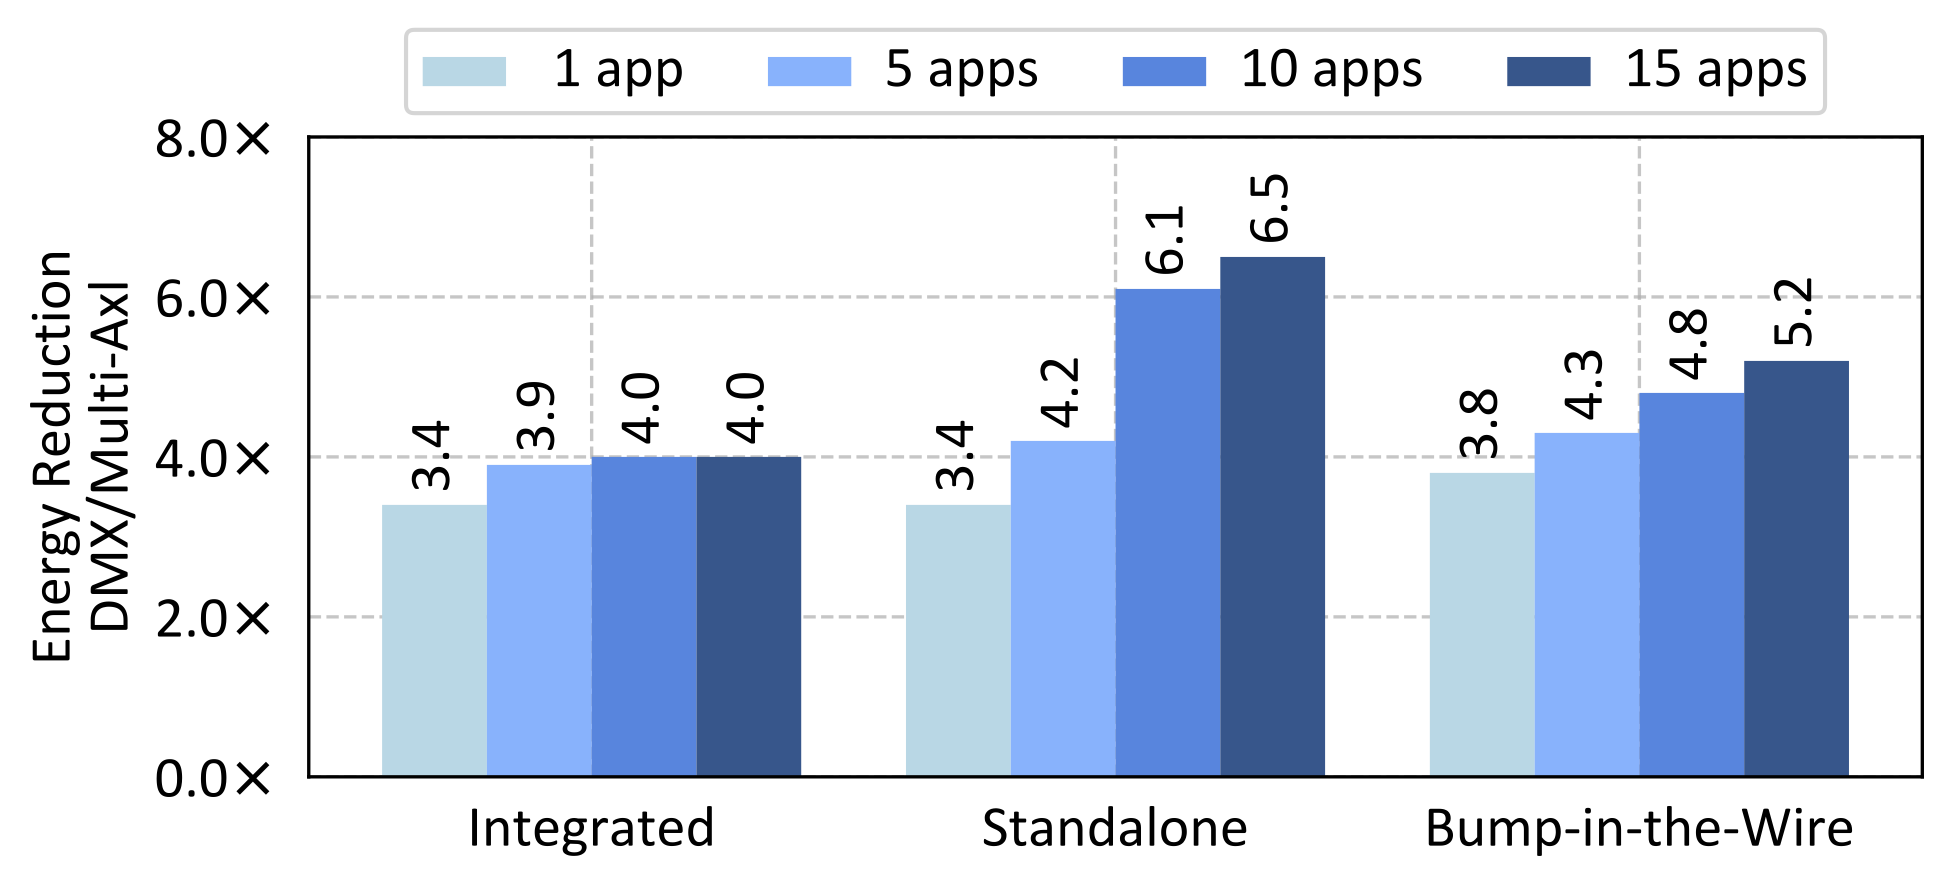
\includegraphics[width=\linewidth]{figure/fianchetto/system-energy-reduction.pdf}
    \caption{System-wide energy reduction, including host CPU cores, accelerators, and \drxs. 
    %
    Bump-in-the-Wire \drx achieves less reduction than Standalone \drx due to its internal PCIe multiplexer shown in Fig.~\ref{fig:drx-config-acc}.
    %
    Integrated, Standalone, and Bump-in-the-Wire \drx draw up to 26\%, 23\% and 28\% more power than the \emph{Multi-Axl} baseline. 
    %
    PCIe-Integrated is not included because we are not able to estimate the power of a \drx-integrated PCIe switch.
    }
    \label{fig:res:energy-drx-placement} 
\end{figure}

\noindent \textbf{Energy reduction with different DRX placements.}
%
Figure~\ref{fig:res:energy-drx-placement} shows system-wide energy reduction provided by different \drx placements compared to \emph{Multi-Axl} baseline.
%
Integrated \drx provides 3.4$\times$, 3.9$\times$, 4.0$\times$, and 4.0$\times$ of energy reduction. 
%
The energy reduction does not scale with the number of concurrent applications because it only benefits from the energy efficiency of the \drx hardware acceleration for data restructuring operations. 
%
Standalone \drx and Bump-in-the-wire \drx provide energy reduction scaling with the increased number of concurrent applications.
%
Bump-in-the-wire \drx placement delivers the best energy reduction of 3.8$\times$ and 4.3$\times$ for 1 and 5 concurrent applications. 
%
Standalone \drx delivers the best energy reduction of 6.1$\times$ and 6.5$\times$ for 10 and 15 concurrent applications because of the reduced bandwidth contention on PCIe links.
%
This is because the extra glue logic and the dual-port PCIe multiplexer are replicated in each Bump-in-the-Wire \drx placement, while such overhead is amortized across the applications on a large Standalone \drx. 
%
PCIe-Integrated is not evaluated for energy reduction because of the difficulty of estimating the energy consumption of a PCIe switch integrated with \drx.
%
\subsection{Sensitivity Studies}
%
\noindent \textbf{Speedup with more than two kernels.}
%
As real-world applications can consist of multiple kernels across domains, it is important for \dmx to scale beyond two kernels. 
%
To evaluate \dmx's scalability with multiple application kernels, 
%
we add a third application kernel to the \pir benchmark, along with its additional data restructuring kernel consisting of reshaping and typecasting. 
%
This third kernel is a Transformer model fine-tuned for Named Entity Recognition (NER). NER identifies personal and sensitive information that is hard to capture for regular expression kernel~\cite{ner-transformer}.
%
We use an open-source BERT implementation for the kernel~\cite{verigoodml:iccad:2021}.
%
% The accelerator takes text as input and performs token embedding lookup on the accelerator like previous BERT implementation on FPGA~\cite{ftrans:ispled:2020}.
%
Figure~\ref{fig:res:multi-kernel}(a) shows the runtime breakdown of this three-kernel benchmark. 
%
Although the benchmark included the compute-intensive NER kernel, the runtime is still dominated by the data restructuring kernels for the \emph{Multi-Axl} baseline.
%
\dmx alleviates the bottleneck of data motion and restores kernel to be the largest contributor that represents 97.2\% to 93.7\% of the end-to-end execution time for one to 15 concurrent applications.  
%
As such, \dmx provides 1.9$\times$ to 4.2$\times$ speedup for one to 15 concurrent applications shown in Figure~\ref{fig:res:multi-kernel}(b).

\begin{figure}[t!]
\begin{subfigure}[ht!]{\columnwidth}
\centering
\includegraphics[width=\columnwidth]{figure/fianchetto/multi-kernel-breakdown.pdf}
\caption{Runtime breakdown}
\label{fig:res:multi-kernel-breakdown}
\end{subfigure}
%
\begin{subfigure}[ht!]{\columnwidth}
\centering
% shifting 
\hspace{-0.75cm}
\includegraphics[width=0.65\columnwidth]{figure/fianchetto/multi-kernel-speedup.pdf}
\caption{Speedup}
\label{fig:res:multi-kernel-speedup}
\end{subfigure}
%
\caption{\dmx reduces data motion overhead to less than 5\% for \pir benchmark extended with Named Entity Recognition kernel.
%\rohan{Shu-Ting when you get some time, please change this color too. Hadi mentioned that he does not like the dark color}
}
\label{fig:res:multi-kernel}
\vspace{-3ex}
\end{figure}

%\revision{
\noindent \textbf{One-to-many and many-to-one data movement.}
%
Cross-domain multi-acceleration of end-to-end applications entails using multiple accelerators.
%
The data movements in multi-acceleration, however, are not necessarily always one-to-one but likely include one-to-many and/or many-to-one data movement between accelerators.
%
Therefore, we want to analyze whether \dmx design can cope with the one-to-many and/or many-to-one data movements in multi-acceleration.
%
To this end, we compare Bump-in-the-Wire \drx against the \emph{Multi-Axl} baseline for one-to-many (i.e., broadcast) and many-to-one (all-reduce) data movement using 4 to 32 accelerators.
%
For broadcast, the baseline first passes the output of the source accelerators to the main memory of the CPU using DMA.
%
%After data restructuring on CPU, the driver clones the restructured data using 8 threads to $N$ DMA buffers and then initiates $N$ DMA transfers to the destination accelerators.
After data restructuring on the CPU, the driver then copies the restructured data and initiates $N$ DMA transfers \emph{sequentially} to the destination accelerators. 
%
All-reduce has two stages: scatter-reduce and all-gather.
%
Both require similar DMA transfers between CPU and accelerators; however, scatter-reduce entails additional steps to first sum the inputs from sources and then scatter the outputs to all destinations. 
%
On the contrary, \dmx's implementation of broadcast and all-reduce utilizes the Bump-in-the-Wire \drx for data restructuring and data movement.
%

Figure~\ref{fig:res:collectives} shows that the \dmx achieves 3.7$\times$ to 5.2$\times$ speedup on broadcast and 5.1$\times$ to 10.5$\times$ speedup for all-reduce on 4 to 32 accelerators.
%
This is because \dmx utilizes \drxs to (1) perform data restructuring and the DMA transfers \emph{in parallel} and (2) eliminate the extra DMA transfers between the accelerators and the CPU.
%
Furthermore, for all-reduce, \dmx uses \drx to accelerate the summation operations.
%
The speedup also scales with the number of accelerators because the amount of data restructuring and data movement scale accordingly to the number of accelerators. 
%
There is a dip when using 16 or more accelerators, but this is due to the additional latency on the PCIe switches that scales with the number of accelerators.
%
\dmx achieved higher speedup in all-reduce compared to broadcast because all-reduce involves more DMA transfers and data restructuring which provided more acceleration opportunity using \drx.
%
% The PCIe switch added to the system when using 16 or more accelerators causes a dip in the relative speedups.
% %
% \dmx achieved higher speedup in All-Reduce compared to broadcast as All-Reduce involves more DMA and memory copy which provided more acceleration opportunity for \dmx.
%
%\dmx's implementation of broadcast and all-reduce avoids PCIe bandwidth contention to the CPU because  Bump-in-the-Wire \drx is local and exclusive to the accelerator.
%
%\dmx also eliminates the extra DMA from accelerators to CPU as well as the memory copy after the data transformation.   
%
%Finally, \dmx uses \drx to accelerate summation operation in the All-Reduce workload.
%
%For inter-accelerator communication, \dmx uses multiple RX/TX data queues on \drx for sending and receiving data from other \drxs as stated in Sec.~\ref{sec:system}.
%
% not this one hanyang. not done yet here.
% \red{This motivates the use of one-to-many and many-to-one data movement between accelerators through \drx in the case of \dmx.} 
%\soroush{why are we doing this experiment? please say that at the beginning}
%Therefore, we compare Bump-in-the-Wire \drx against the \emph{Multi-Axl} baseline for one-to-many (i.e., broadcast) and many-to-one (all-reduce) data movement using 4 to 32 accelerators.
%
%The multi-acceleration baseline orchestrates inter-accelerator operations through CPU and main memory.
%
%For broadcast, the baseline first passes the output of the accelerator to the host CPU's main memory through DMA.
%
%After data transformation, the driver clones the transformed data using 8 threads to $N$ DMA buffers and then initiates $N$ DMA transfers to the destination accelerators. 
%Then, it makes $N$ copy, which $N$ is the number of receiving accelerators, to buffer corresponding to each receiver. The memory copy operation is parallelized by 8 threads. Lastly, it DMAs the $N$ copy to the corresponding accelerator.
%
%For all-reduce, the workflow is similar except it has twice as many memory copies on per-accelerator DMA buffers in the two stages of all-reduce: scatter-reduce and all-gather.
%For all-reduce, the workflow is similar except it has twice amount of memory copy on per-accelerator buffers in the two stages of all-reduce: scatter-reduce and all-gather.
%
% \dmx's implementation of broadcast and all-reduce avoids PCIe bandwidth contention to the CPU because  Bump-in-the-Wire \drx is local and exclusive to the accelerator.
% %
% \dmx also eliminates the extra DMA from accelerators to CPU as well as the memory copy after the data transformation.   
% %
% Finally, \dmx uses \drx to accelerate summation operation in the All-Reduce workload.
% %
%As such, \dmx achieves 3.7$\times$ to 5.2$\times$ speedup on broadcast and 5.1$\times$ to 10.5$\times$ speedup for all-reduce on 4 to 32 accelerators shown in Figure \ref{fig:res:collectives}
%Therefore, \dmx achieves 5.2 $\times$ and 10.4 $\times$ latency improvement on 32 accelerators for broadcast and all-reduce respectively.
%\malian{why doing a simple summation results in such a huge gap in the relative speedup?}
%
%\revision{
%
%The overall improvement scale with the number of accelerators because the amount of data movement scale accordingly to the number of accelerators. 
%
%The PCIe switch added to the system when using 16 or more accelerators causes a dip in the relative speedups.
%
%\dmx achieved higher speedup in All-Reduce compared to broadcast as All-Reduce involves more DMA and memory copy which provided more acceleration opportunity for \dmx.
%

\begin{figure}[t!]
    \centering
    %\includegraphics[width=0.8\columnwidth, cframe=blue!5!blue 0.5mm]
    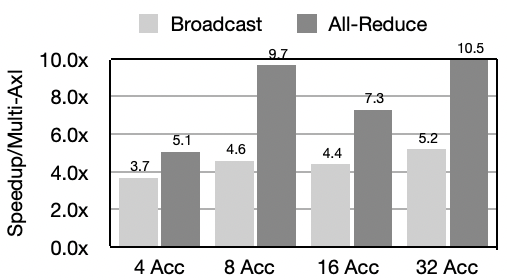
\includegraphics[width=\columnwidth]{figure/fianchetto/collectives.pdf}
    \caption{\dmx eliminates redundant DMA transfers and performs DMA in parallel for broadcast and all-reduce on multi-accelerator setup.}
    \label{fig:res:collectives}
\end{figure}

% \begin{figure}[t!]
%     \centering
%     \includegraphics[width=\columnwidth]{ASPLOS23/figures-resubmit/standalone-underprovision.pdf}
%     \caption{End-to-end latency speedup of different provision levels of Standalone \drx. 
%     Over-provisioning \drx is better in terms of performance and energy consumption because under-provisioning \drx yields lower speedup and uses 1.2$\times$ to 1.4$\times$ more energy.
%     }
%     \label{fig:res:stnadalone-underprovision}
% \end{figure}

% \noindent \textbf{Provision levels of standalone \drx.}
% %
% While deploying end-to-end applications as a service, the Total-Cost-of-Ownership (TCO) is critical to the system design~\cite{e3:atc:2019}.
% %
% The provision levels of Standalone \drx are important as lower levels of provisioning provide lower purchase prices and operating costs.
% %
% Therefore, lowering the provision levels of \drx may be a luring choice when only a few applications are running.
% %
% However, it is important to note that we must make sure that the latency of the end-to-end application stays within the margin.
% %
% To this end, we analyze the impact of different provision levels of \drx.
% %
% The over-provisioned configuration of Standalone \drx provisions just one more Standalone \drx than its need of data restructuring computation.
% %
% The under-provisioned configuration, on the other hand, provisions one less Standalone \drx it needs. The two provision levels do not match the demand for data restructuring but are close to the right-sized provision.
% %
% Over-provisioned Standalone \drx leads to utilization on various levels: 25\%, 62.5\%, 83.3\%, and 93.8\% for 1, 5, 10, and 15 concurrent applications, respectively.
% %
% Under-provisioned Standalone \drx does provide full utilization but it also leads to 16.6\% and 21.6\% lower speedup than the over-provisioned counterpart for 10 and 15 concurrent applications.
% %
% The lower speedup of under-provisioned Standalone \drx is due to increased contention on bandwidth to access \drx.
% %
% This also results in 1.2$\times$ to 1.4$\times$ more energy consumption than its over-provisioned counterpart, though it uses a fewer number of PCIe switches and Standalone \drx.
% %
% Overall, over-provisioning \drx is better in terms of performance and energy consumption.  
%
% \hanyang{I think this is not a well thought-out experiment in general. First, how do you even define under-provision? you can have 1 DRX for 15 applications or 3 DRXs for 15 applications and both of those could still be under-provisioned for the use case, so which result should you report in this case? Generalizing it under one category feels like an over-simplification. Second, CPU-Integrated DRX could also be facing contention, it is not clear what exactly is the problem under study here, what exactly is causing the slowdown in this experiment? I think it is even a little bit trivial since of course you are gonna have some kind of contention when you over-utilize the DRX. My opinion is to delete this section altogether}


%\begin{comment}

\begin{figure}[t!]
    \centering
    \includegraphics[width=\linewidth]{figure/fianchetto/sensitivity-simd-lanes.pdf}
    \caption{Data restructuring latency speedup with different numbers of RE lanes on \drx. The increase of speedup
    is limited after 128 lanes. which is our default configuration.}
    \label{fig:res:simd-lanes}
\end{figure}

\begin{figure}[t!]
    \centering
    %\includegraphics[width=1\columnwidth, cframe=red!5!red 0.5mm]{ASPLOS23/figures-resubmit/drx-acc-arch.pdf}
    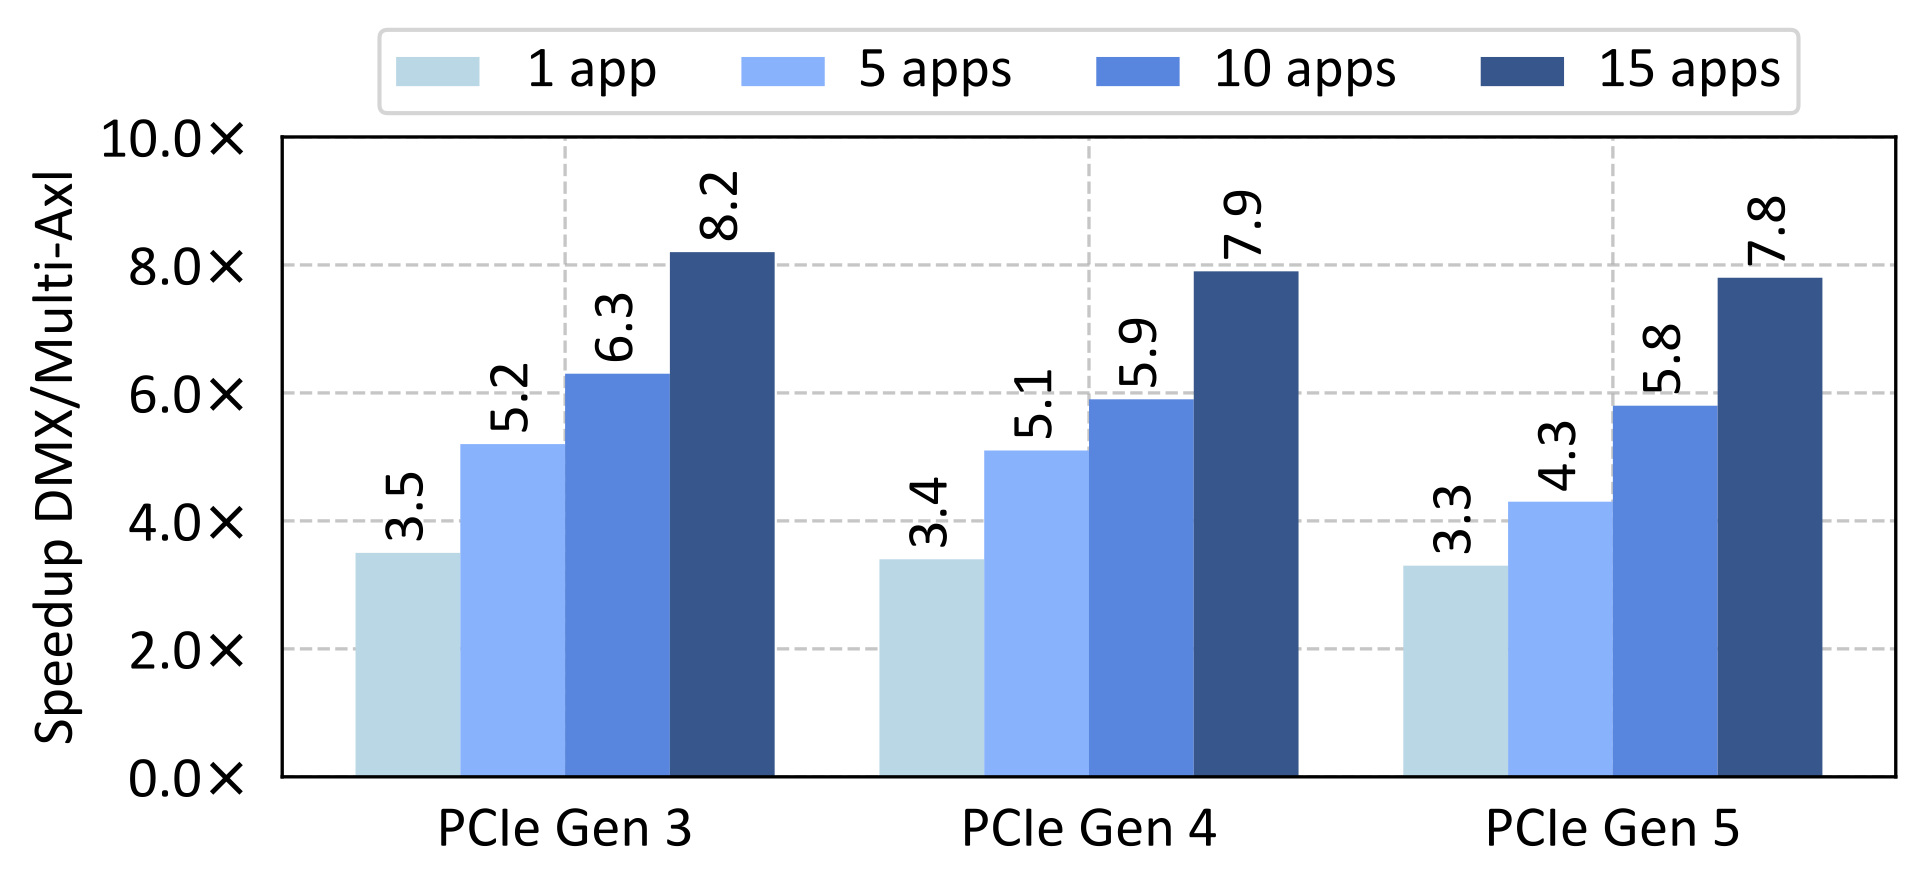
\includegraphics[width=0.98\columnwidth]{figure/fianchetto/speedup-diff-pcie-gens.pdf}
    \caption{\dmx speedup across generations of PCIe. PCIe Gen4 and Gen5 result in a slight decrease of speedup because their corresponding \emph{Multi-Axl} baselines improve more than their \dmx counterparts.}
    \label{fig:res:pcie-gens}
\end{figure}


\noindent \textbf{DRX hardware configurations.}
\label{sec:results:hardware-config}
%
To understand the sensitivity of \dmx to the amount of compute resources in \drx, we sweep the number of RE lanes for \drx and compare its performance to the \emph{Multi-Axl} baseline that performs data restructuring on CPU. 
%\soroush{why 16? is it different fron the baseline config that we used to show the speedup numbers? if yes, why?}.
%
% The default configurations used throughout the experiments are 128 vector lanes and 64KB of data scratchpad.
% %
%\noindent \textbf{Sensitivity Analysis: SIMD lanes.}
Figure~\ref{fig:res:simd-lanes} shows the speedup achieved for the different number of lanes for \drx: from 32 to 256. 
%
The speedup improves with the number of lanes increasing up to 128 lanes by taking advantage of available data parallelism in data restructuring operations.
%
%\rohan{from the figure, it does not seem like the speedup saturates}
%
However, the increase of speedup of \drx is limited after 128 RE lanes, and increasing the lanes to 256 does not provide noticeable benefits.
%
Therefore, we use 128 RE lanes as the default configuration for \drx throughout the experiments. 
%as the optimal point for performance.
%\end{comment}


\noindent \textbf{Different PCIe generations.}
Newer PCIe generation provides significantly more bandwidth and the increased bandwidth can potentially negate the performance benefit of \dmx. 
%
To understand the impact of different generations of PCIe, we compare the Bump-in-the-Wire DRX latency speedup on PCIe Gen 3 with PCIe Gen 4 and Gen 5.
%
Figure \ref{fig:res:pcie-gens} shows that using PCIe Gen 4 and Gen 5 resulted in a slight decrease of speedup because their corresponding \emph{Multi-Axl} baselines improve more than their \dmx counterparts.
%
Across PCIe generations, the baselines and \dmx show different levels of improvement only in data movement latency. 
%
Such differences come from the following two reasons.
%
First, the baselines face more bandwidth contention than the \dmx and thus benefit more from the increased PCIe bandwidth per lane.
%
Second, the baselines are able to use more PCIe lanes to reduce bandwidth contention from accelerators to CPUs with PCIe Gen 4 and Gen 5 compared to CPUs with PCIe Gen 3~\cite{intel-cascade-lake, intel-ice-lake, intel-sapphire-rapids}. The results shown in Figure~\ref{fig:res:pcie-gens} suggests that the bottleneck of \emph{Multi-Axl} configuration is not just the PCIe interconnect, but also the data restructuring computation. 

%\begin{comment}
% \begin{figure}[ht]
%     \centering
%     \includegraphics[width=\columnwidth]{figure/fianchetto/cxl-cpu-solutions.pdf}
%     \caption{CXL shows negligible slowdown on the multi-acceleration baseline over PCIe. Integrated \drx which integrates \drx on CPU shows similar speedup on PCIe and CXL.}
%     \label{fig:res:cxl-cpu-solutions}
%     \vspace{-2ex}
% \end{figure}
%
% \noindent \textbf{CXL as Interconnect Alternative.}
% %\subsection{Interconnect Alternative: CXL}
% %\label{sec:results:cxl}
% %\stingw{again, why on earth do we want to do this? we can say this reduce the control overhead, e.g. interrupts and scheduling. CXL translate that to a cache coherency problem.}
% % CXL~\cite{cxl-3-0-spec} is an interconnect alternative that can reduce the control overhead, such as interrupts, for multi-acceleration systems. CXL translates the overhead of the non-coherent DMA approach to cache coherency overhead.
% CXL~\cite{cxl-3-0-spec} is an interconnect alternative that can reduce the control overhead, such as interrupts, for multi-acceleration systems with attached expandable coherent memory systems. CXL trades off the overheads of the non-coherent DMA approach with overheads for supporting cache coherency.
% %
% Both multi-acceleration and Integrated \drx with CXL shows no improvement and a negligible slowdown in Fig.~\ref{fig:res:cxl-cpu-solutions}. 
% %
% The accelerators in our benchmarks are fed with input data between 6$\sim$16 MBs as they do not operate on the granularity of a cache line. Therefore, CXL provides no tangible benefit to our benchmarks running with \dmx.
% %
% This observation is consistent with prior work~\cite{cxl-model:exhet:2022} modeling CXL which is calibrated with GPU and FPGA measurements. They observed CXL outperforming PCIe only for transfers less than 12.7 KB and with frequent host-accelerator interactions. 

% The energy efficiency of \drx is the primary reason for energy reduction shown for a single application as
% \drx consumes less power and performs data restructuring operations more efficiently than CPU. 
% %
% Integrated \drx draws more energy than the other two placement strategies.
% %
% Integrated \drx runs longer as shown in its less latency speedup in Fig.~\ref{fig:res:speedup-drx-placement}. This keeps PCIe switches and \drx active for a longer period of time and results in the worst energy reduction among the three.
% %
% Standalone \drx consumes less energy than Integrated \drx because of its better speedup. 
%\end{comment}


% \vspace{-1ex}
\section{Related Work}
\label{sec:related}
%
Real-world applications span multiple domains, posing a challenge for end-to-end acceleration.
%
While the research community has explored accelerators across diverse domains~\cite{q100:asplos:2014, meet-the-walkers:isca:2013, doppiodb:fpl:2017,chiosa:pvldb:2022, acc-yolov3:iscas:2020, wfa:fpl:2021, genstore:asplos:2022, segram:isca:2022, meet-the-walker:micro:2013,murray:micro:2016,robox:isca:2018,pointacc:micro:2021,robomorphic:asplos:2021}, the adoption of these heterogeneous accelerator to accelerate a single end-to-end application is challenging.
%
The challenge arises due to the diverse data formats generated and consumed by each accelerator.
%
This necessitates restructuring inputs and outputs across accelerators. 
%
While some prior works have focused on performed data restructuring using CPUs, this paper introduces the concept of Data Motion Acceleration (DMX) for efficient cross-domain multi-acceleration with heterogeneous DSAs.
%
We review the most relevant related work in three areas: data movement, data restructuring, and interconnect fabrics integration below.
%

\noindent \textbf{Data movement.}
%
Prior works studied point-to-point data movement between GPUs~\cite{gpudirect:2019}, between GPU and storage~\cite{morpheus:isca:2016,spin:atc:2017,nds:micro:2021}, between NIC and accelerator~\cite{p2pdma:apsys:2020,lynx:asplos:2020,flexdriver:asplos:2022}, and between on-chip accelerators~\cite{arc:dac:2012}. 
%
Prior works have used various techniques such as scheduling~\cite{wisefuse:sigmetrics:2022, mahapatra:mlarchsys:2022, paragon:asplos:2013, lynx:asplos:2020,flexdriver:asplos:2022} to co-locate multiple domains on the same system. 
%
While these works only optimize the data movement, non-trivial operations of the data restructuring still consumes a significant fraction of the data motion.
%
Intel Data Stream Accelerator~\cite{intel-dsa} and DCS~\cite{dcs:micro:2015, dcs-ctrl:isca:2018} share a similar insight, both lack programmability and hence have limited capacity to optimize data restructuring.
%
This work in contrast leverages \drxs as a compute-enabled glue that links different heterogeneous accelerators together and makes them appear as a monolithic but composable accelerator for the application.
%

\noindent \textbf{Data restructuring.}
%
For message serialization, Optimus Prime~\cite{optimusprime:asplos:2020} and Protobuf accelerator~\cite{protobuf:isca:2021} design an accelerator for RPC message serialization.
%
HGum~\cite{hgum:reconfig:2017} and Fletcher~\cite{peltenburg-2019-fletcher} implement serialization on FPGAs for acceleration.
%
For machine learning pipelines, tf.data~\cite{tf.data:pvldb:2021}, DSI~\cite{dsi-dlrm:isca:2022}, DALI~\cite{nvidia-dali:2018} optimize data restructuring on GPU with programmable operations.
%
In contrast to these prior works that only optimize data restructuring for a single accelerator, this paper investigates data restructuring and movement for multi-acceleration with heterogeneous devices.
%

\noindent \textbf{Interconnect fabrics.}
%
Previous works have used PCIe's Non-Transparent Bridge (NTB) to enable PCIe to support multiple hosts with more than one root complex, which performs address translation for operations in a specific memory range~\cite{hou:hpca:2013,smartio:tocs:2021}.
%
Point-to-point DMA over PCIe fabric is enabled by a shared address space across all devices~\cite{gigaio-pcie-swtich}.
%
CXL 3.0 or later allows accelerators on different servers to be connected seamlessly by using fabric switching to link racks of devices and accelerators~\cite{cxl-3-0-spec}.    
%
DUA~\cite{dua:nsdi:2019} creates an overlay fabric on top of the existing physical communication stacks, such as PCIe, Ethernet, DDR, etc.
%
These works can connect accelerators without addressing data restructuring for multi-acceleration.
%
This work, however, tackles data motion challenges to maximize the performance of multi-acceleration.

\section{Conclusion}
\label{sec:conclusion}
%
% With heterogeneous data centers, while accelerators are becoming a prominent component, there is a need for considering issues that arise in the intersection of system and architecture.
In this work, we quantified the data motion cost of chaining heterogeneous domain-specific accelerators for multi-acceleration.
%
The results showed that the data motion overhead curtails the end-to-end speedup of accelerating each domain on a set of heterogeneous accelerators. 
%
The paper introduced \dmx that seamlessly weaves together multiple accelerators that deliver the performance of a large, monolithic cross-domain accelerator. 
%
On average, \dmx provides between 3.4$\times$ to 8.2$\times$ speedup, 3.0$\times$ to 13.6$\times$ higher throughput, and 3.8$\times$ to 5.2$\times$ energy reduction.

Even with current single-domain accelerators, overheads of moving data on- and off-chip is presently a dominant factor that limits the performance and energy efficiency of gains~\cite{horowitz:isscc:2014, accelerator-cluster:hoti:2023}. 
%
The impact of the data motion--highlighted in this paper--will worsen when cross-domain accelerators are chained in future datacenters to cater to the requirements of emerging end-to-end applications.
%
This even includes the multimodal generative AI applications that use multiple models and require acceleration beyond neural networks (e.g., vector database lookups, search, etc.).
%
Heterogeneous/3D integration coupled with emerging high-bandwidth chiplet-to-chiplet interconnects such as UCIe can improve data movement, but not data restructuring that requires computation.
%
As such, embedding our \dmx concept and architecture within these interconnects can synergistically unlock the the potential of cross-domain multi-acceleration for next-generation dataceneters.

\section{Sources for Material Presented in This Chapter}
%
Chapter~\ref{fianchetto:chap}, in part, reprints material as it appears in a paper titled: "Data Motion Acceleration: Chaining Cross-Domain Multi Accelerators"
by Shu-Ting Wang, Hanyang Xu, Amin Mamandipoor, Rohan Mahapatra, Byung Hoon Ahn, 
Soroush Ghodrati, Krishnan Kailas, Mohammad Alian, and Hadi Esmaeilzadeh~\cite{dmx:hpca:2024}.
% 
The dissertation author was the primary researcher and author of this material.
\chapter{Aurelia: CXL fabric in making}
\label{aurelia:chap}

\section{Introduction}
%\stingw{the idea is to use CXL fabric as the next-gen rack-scale fabric for disaggregation/composable systems.}
%\stingw{why do we need CXL at the first place? disaggregation and composable system}
The datacenters move towards disaggregated and composable infrastructure, in which different resources are taken from a logical pool to satisfy the demand from applications.
%
%Existing effort of disaggregation relies on RDMA over Ethernet, a fabric not designed with disaggregation in mind. 
Existing effort retrofits the current Ethernet fabric for disaggregation by running RDMA over Ethernet~\cite{legoos:osdi:2018, far-memory:eurosys:2020, leap:atc:2020,aifm:osdi:2020,carbink:osdi:2022,hydra:fast:2022,canvas:nsdi:2023}.
%
However, retrofitting existing hardware prevents applications from reaching their optimal performance under disaggregation and sometimes demonstrates inferior performance than its counterpart with server-based setups.

Recent works look toward co-designing hardware with software to realize disaggregation~\cite{kona:asplos:2021, intel-cxl:ieee-micro:2023, tpp:asplos:2023, pond:asplos:2023}.
%
These works are focused on externalizing the hardware interconnect to become a fabric connecting many devices in a disaggregated setting.
%
Fabrics directly connect all the devices allowing accessing remote devices to be similar to accessing a local device on a server's PCIe slots.  
%
PCIe is an example of this kind of fabric, but it only connects local devices within a server right now.
%
% For inter-server communication, PCIe is mainly used to pass data to NIC that further passes the data over Ethernet. 
%
%\stingw{PCIe can go across servers with non-transparent bridge but it's hardly used.}
%
An ideal fabric for disaggregation offers direct connections between devices while providing low latency and high bandwidth on a specific scale, e.g. a single rack or a few neighboring racks.
%rich semantics beyond PCIe's I/O semantics 

Compute Express Link (CXL) emerges as a viable candidate supported by a converged industry standard after its absorption of OpenCAPI and Gen-Z. 
%
CXL is built on top of PCIe with the addition of memory accessing semantics (CXL.mem), caching semantics (CXL.cache), and peer-to-peer memory access between devices (Unordered I/O in CXL.io). 
%
% \stingw{CXL-capable devices use load/store to access everything without any software layering}
%
More importantly, CXL can be a fabric through its support of multi-level switching.

Experimental CXL fabric demonstrates on-par performance with lower cost in the case of machine learning model training on 10s of GPUs~\cite{fabric-saving}. 
%
CXL fabric offers bandwidth as high as 63 GB/s with PCIe 5.0 now and 121 GB/s PCIe 6.0 on the horizon of the next two years~\cite{pcie-6-7}.
% https://www.xda-developers.com/pcie-6-to-launch-in-2024-pcie-7-in-2027/
%
%CXL fabric is able to offer performance benefit from the fabric adoption atop of proper right-sizing of hardware due to disaggregation.
%
CXL fabric offers low latency because it operates on a device-attached interface using direct load/store instructions.
%to avoid additional interface transition. 
%(CXL $\rightarrow$ CXL). 
%
It avoids the network software stack overhead and the PCIe transition between device and NIC on the sending (Device $\rightarrow$ PCIe $\rightarrow$ NIC) and receiving (NIC $\rightarrow$ PCIe $\rightarrow$ Device) path.
%
Network stack and PCIe transition create latency overhead and throughput bottleneck.
%
First, the network stack using kernel bypassing still incurs microseconds of latency overhead~\cite{shinjuku:nsdi:2019, shenango:nsdi:2019, eRPC:nsdi:2019,snap:sosp:2019}.
%
Second, the PCIe latency overhead of 1500 B packets reaching the wire can be as high as 77\%~\cite{pcie-bench:sigcomm:2018}.
%
Third, the PCIe link to NIC is a potential throughput bottleneck when multiple devices share the NIC.
%
Dedicating a NIC for each device circumvents the throughput bottleneck but with the increased cost on more NICs and switches.

%\vspace{-1ex}
\section{Motivation and Background}
\label{aurelia:sec:motivation}

\subsection{What is CXL?}
Compute Express Link (CXL) emerges as an enhancement of PCIe providing cache coherency (CXL.cache), host-managed or fabric-attached memory (CXL.mem), peer-to-peer memory access between I/O devices (CXL.io).
%
CXL.mem provides host-managed memory that CPU and accelerators are able to read/write into each other's memory directly. This avoids redundant DMA operations moving data back and forth~\cite{fulcrum:hpca:2020, beacon:micro:2022, intel-cxl:ieee-micro:2023}.
%
CXL.mem enables fabric-attached memory providing a shared memory pool for applications with different demands~\cite{cxl-ssd:hotstorage:2022, directcxl:atc:2022, pond:asplos:2023}.
%
CXL.cache supports a fully coherent cache on devices with their hosts. These devices, however, do not open their local, private memory to CXL. 
%
CXL.io uses unordered I/O for peer-to-peer memory accesses between non-coherent devices over its fabric.
%
%CXL.io supports non-coherent data movement with I/O devices like PCIe does.

\noindent \textbf{Fabric Routing.}
CXL routes packets with a per-device ID called Port ID on the fabric. 
%
The Port ID-based routing (PBR) addresses each device with a 12-bit ID. 
%
A packet with PBR contains a specific source port ID and destination port ID before it leaves an edge CXL switch that connects directly with devices.
%
Each CXL fabric has a single fabric manager to initialize, bind/unbind devices to ports, and handle event notifications, such as the removal or failure of devices, from the switch.   
%
This fabric manager is very close to a centralized network controller because it controls the per-port forwarding and is aware of all the route changes. 

\noindent \textbf{Flow control.}
CXL inherits point-to-point flow control from PCIe that was designed for the communication between the device and CPU rather than a fabric. 
%
The flow control operates between two directly connected endpoints. 
%
They exchange credit tokens to evaluate the available buffer space on each side. 

\noindent \textbf{QoS Telemetry:.}
CXL fabric offers rate throttling mechanism for hosts called QoS Telemetry. 
%
It is used for devices with its local memory including memory expansion devices and accelerators with device memory, e.g. GPU, FPGA, and ASIC.
%
QoS telemetry enables memory devices to indicate their current internal load with 2 bits for CXL.mem response packets.  
%
The senders use the reported internal load to monitor and throttle their request rate to avoid device overload and possible fabric congestion. 
%
The rate throttling targets specifically for devices, mainly memory devices, that are associated with a host in the current design. 
%
In addition, QoS telemetry devises a mechanism called Egress Port Backpressure (EP Backpressure).
%
It monitors the flow control backpressure situation on each CXL switch egress port. 
%
If the port cannot transmit packets for a period of time due to the lack of credits, the port marks EP Backpressure value in 2 bits on the device load field of the outgoing request. 
%
The overall load of a device is determined by the maxima of device internal load and EP Backpressure. 

\subsection{What is Different with CXL Fabric?}
% \stingw{1. latency (synchronous request) and scalability (cache coherence plague + routing + transport)}
CXL fabric exposes memory traffic that used to be internal to a server to all endpoints connecting on the fabric. 
%
The memory traffic, such as cache coherence, memory access, and I/O style accesses, runs between processor and device endpoints on CXL fabric.
%
This is in contrast to standard data center traffic running with encapsulated packets from per-server NIC outside of the internal memory fabric of a server.
%
Processors and accelerators access remote devices with load/store instructions through CXL fabric.
%
They synchronously request data from remote devices, e.g. memory expansion modules, accelerators, and storage devices. 
%
However, these synchronously request data cannot tolerate significant latency, because the latency will 
stall the execution of the requester hardware while awaiting the requested data.
%
This poses restricted latency requirements for the fabric and needs proper system-level support. 
%
Additionally, CXL fabric allows up to 4096 endpoints.
%
Given the scale of 1000s of endpoints and the mixture of memory traffic,
this introduces a challenge on the scalability of the underlying protocol design.
%
%\stingw{
A centralized scheduler is a possible solution for 10s or even 100s of endpoints on racks.
%
However, the scheduler is very likely to be the performance bottleneck because it needs to sustain and determines the order of every load/store instructions.
%
The scheduler can become a single point of failure for all memory traffic.
%
The scheduler with a centralized design in mind limits the scalability for CXL using longer distanced physical layer than PCIe.
%}
% \TODO{Why not just make it a scheduler instead of distributed protocols?}
% \stingw{We try tot argue this qualitatively.}
%
To understand the practical challenges, use cases of CXL fabric from CXL specification and the literature are discussed next~\cite{cxl-3-0-spec, directcxl:atc:2022, pond:asplos:2023}. 
%

\subsection{Use Cases of CXL Fabric}
\label{aurelia:subsec:use-cases}
The use cases of CXL fabrics demand large memory capacity, high bandwidth, and low latency.
%
Emerging and existing workloads in data centers, such as machine learning models, 
large-scale key-value stores, and high-performance computing (HPC) applications, can benefit from CXL fabrics.   

% Moreover, CXL fabric provides an alternative to Nvidia's proprietary stack (NVLink + NVSwitch + Infiniband RDMA).
% %
% CXL fabric will enable future accelerators to connect and cooperate on applications on a shared, open-standard communication substrate
% instead of using only GPUs.
%
% \TODO{cite NERSC's Arxiv report to argue for the need of disagg with concrete numbers.}
%
%HPC uses a topology like model training but featuring different 
% Host CPU cores are connected with accelerators and accessing fabric-attached memory for additional memory capacity and bandwidth~\cite{memory-trend:snl:2020, hpc-disagg-mem:arxiv:2023} (Shown in Figure~\ref{fig:ml-acc-cxl}).
% Previous works proposed to leave these out of accelerators onto main memory but with potential slowdown caused by explicit memory copying from memory to accelerators~\cite{zero-infinity:sc:2021, zero-offload:atc:2021, deepspeed-inference:sc:2022}.

First, the current machine learning models require a large amount of memory on an accelerator, e.g. GPU or TPU, which is beyond the capacity of individual accelerators.
%
To make it even worse, the size of state-of-the-art machine learning models are ranged from 10s of GB to 10s of TB.~\cite{zero:arxiv:2020, zero-infinity:sc:2021, zionex:isca:2022} and keep growing every few months.
%
Training and inference of machine learning models now need multiple accelerators to jointly fit the model and intermediate variables in their memory. 
%
CXL fabric could expand accessible memory to accelerators by providing fabric-attached memory.
%
Fabric-attached memory increases the memory capacity and bandwidth to all available memory on the fabric~\cite{cxl-3-0-spec, samsung-memory-expander:hcs:2022, memory-scalability:microchip}.
%
%A topology of this model training use case is shown in Figure~\ref{fig:ml-acc-cxl}. 
%
A host is connected with an accelerator with CXL and they share a coherence domain (Shown in Figure~\ref{fig:ml-acc-cxl}).   
%
Accelerators access the fabric-attached memory and each other's memory in a producer-consumer fashion of I/O coherency.
%

Second, the datacenter runs cloud services with key-value stores.
%
Key-value stores use RDMA inside datacenter to speed up the communication and operations~\cite{farm:nsdi:2014,herd:sigcomm:2014,eRPC:nsdi:2019, xstore:osdi:2020}
%
These operations are sensitive to latency and are on the performance critical path of applications. 
%
DirectCXL showed CXL to be 8.3x shorter latency than RDMA for 64B read and replacing RDMA with less overhead~\cite{directcxl:atc:2022}. 
%CXL is able to replace RDMA with less overhead as DirectCXL suggested~\cite{directcxl:atc:2022}. 
%
DircetCXL provides a latency lower bound of CXL because its fabric has a single switch and is not under stress or congestion.
%
The hosts do not maintain cache coherence between themselves. Fabric-attached memory module maintains coherence between itself and the host address space it has mapped (Shown in Figure.~\ref{fig:kvs-cxl}).

Third, HPC workloads demonstrate high utilization ($>$ 90\%) on memory bandwidth as well as capacity for representative applications~\cite{doe-miniapps, crossroad-benchmarks, exascale-apps}. 
%
Though each application stays with its peak memory usage for a different duration of time.
%
The cluster is required to be provisioned to the peak bandwidth and capacity to avoid significant slowdown~\cite{hpc-memory-requirement:upc:2019, memory-trend:snl:2020, hpc-disagg-mem:arxiv:2023}.

Machine learning and HPC workload both involve collective communication while key-value stores involve bursty non-structural communication.
%
Collective communication is structural and can be optimized with data prefetch to minimize the stall on pending memory accessing.
%
This relaxes their requirement on latency and reduces burstiness.
%
Training and inference of machine learning models use all-reduce to update model weights to each accelerator after each iteration. The size of state-of-the-art models is ranged from 10s of GB to 10s of TB.~\cite{zero:arxiv:2020, zero-infinity:sc:2021, zionex:isca:2022}.
%
HPC compared to machine learning has a more diverse communication pattern, such as sweeping or nearest-neighbors~\cite{mpi-usage:sc:2019, ember-comm, exascale-apps, doe-miniapps}. 
%
Key-value store and database, however, serve bursty requests and are sensitive to latency~\cite{scale-memcache:nsdi:2013, rocksdb-modeling:fast:2020}

\begin{figure}[ht!]
%%%%
    \begin{subfigure}[ht]{0.8\columnwidth}
    \centering{
    \includegraphics[width=\columnwidth]{./figure/aurelia/ml-acc-cxl-fabric.pdf}
    \caption{Machine learning and HPC. Hosts and their accelerators share a coherent domain.}
    \label{fig:ml-acc-cxl}
    }
    \end{subfigure}

    \begin{subfigure}[ht]{0.8\columnwidth}
    \centering{
    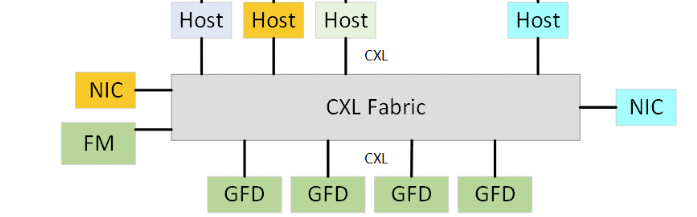
\includegraphics[width=\columnwidth]{./figure/aurelia/kvs-cxl-fabric.pdf}
    \caption{Key-value store for cloud services.}
    \label{fig:kvs-cxl}  
    }
    \end{subfigure}
\caption{CXL fabric abstractive topology.}
\label{fig:cxl-topo}
\end{figure}

% \begin{table}[ht!]
% \begin{tabular}{|l|l|l|l|}
% \hline
%             & Bandwidth & Latency & Burstiness         \\ \hline
% Machine Learning Models & +         & $\triangle$    & -           \\ \hline
% High Performance Computing        & +         & $\triangle$    & $\triangle$ \\ \hline
% Key-value Store    & -         & +              & +           \\ \hline
% \end{tabular}
% \caption{Traffic patterns for different workloads.}
% \label{tab:cxl-workload}
% \end{table}

\section{Challenges}
% \begin{comment}
% list out the challenges related to scalability and latency
% latency     -> congestion control, long stall
% scalability -> routing, coherence traffic monitoring + restriction if possible     
% \end{comment}
%
The current design of CXL fabric~\cite{cxl-3-0-spec} poses challenges on scalability and latency. 
%
First, its addressing and routing design limits the possibility of flexible and dynamic routing. 
%
Second, the lack of an end-to-end transport layer of the fabric makes the fabric prone to congestion and latency spikes. 
%
More importantly, with the usage of load/store instructions, the processor and accelerator that synchronously request data are very sensitive to latency because the latency determines how long they need to stall their execution.
%
The addressing, routing, and transport-level challenges are discussed in the following subsections.  

\subsection{Addressing and Routing Challenges}
\label{aurelia:sec:motivation:routing}

%\noindent \textbf{Routing.}
CXL routes packets with a per-device ID called Port ID on the fabric. 
%
The Port ID-based routing (PBR) addresses each device with a 12-bit ID. 
%
A packet with PBR contains a specific source port ID and destination port ID before it leaves an edge CXL switch that connects directly with devices.
%
Each CXL fabric has a single fabric manager to initialize, bind/unbind devices to ports, and handle event notifications, such as the removal or failure of devices, from the switch.   
%
The fabric manager is equivalent to a centralized software-defined network controller as it controls the per-port forwarding and is aware of all the route changes. 
%
However, CXL fabric has (1) a limiting addressing scheme to support multi-path and adaptive routing, %address devices under multi-level switching
(2) single-path and inactive routing regardless of the traffic condition.

%However, the current CXL routing falls short to achieve its own expectation because of the following reasons.
\noindent \textbf{Challenge: Limited addressing support for multi-path and adaptive routing.}
%
% \stingw{ Yes multi-level routing is feasible with CXL 3.0.
% But SPID and DPID are only used to describe devices.
% The fabric routing is SDN-style, so all routing reconfiguration (with packet sparying or load aware) needs to go through Fabric Manager. This make FM a performance bottleneck.
% }
%
The current PBR routing scheme assigns an ID to devices only. 
%
PBR routes packets to the destination device through multi-level switches with routing installed by the fabric manager. 
%
Any routing reconfiguration needs to go through the fabric manager and thus making load-aware, adaptive routing inefficient and infeasible on a large scale.
%
%PBR with routes controlled by the fabric manager 
The centralized routing of PBR prevents the usage of classic multi-pathing techniques like packet spraying or ECMP because all the routes are pre-determined by the fabric manager.
%
Figure.~\ref{fig:cxl-fabric-overview} shows an example of multi-level CXL fabric.     
%
%if the fabric does not have inter-switch links with a single-level switching.
%
% PBR prevents CXL fabric to realize the multi-level switching that enables a larger topology with switches connected.
%
%PBR cannot route packets through this because it does not address the switches on the fabric.  

\noindent \textbf{Challenge: inflexible routing over diverse topologies.}
CXL fabric supports flexible topology and thus opens the possibility of having a wide range of topologies such as a fully connected graph, Fat-tree~\cite{fat-tree:sigcomm:2008} or Dragonfly~\cite{dragonfly:isca:2008}. 
%
These topologies provide multiple paths for a source and a destination, but CXL fabric cannot route packets over multiple possible paths given its current design.

\subsection{Transport-level Challenges}
\label{aurelia:sec:motivation:transport}
% The transport of CXL includes PCIe for point-to-point flow control and QoS Telemetry implementing ad hoc rate-throttling for CXL.mem traffic. These two mechanisms are not able to ensure a predictable fabric latency with minimal congestion.  

CXL inherits point-to-point flow control from PCIe that was designed for the communication between the device and CPU rather than a fabric. 
%
The flow control operates between two directly connected endpoints. 
%
They exchange credit tokens to evaluate the available buffer space on each side. 
%

\begin{figure}[t!]  
    \centering
    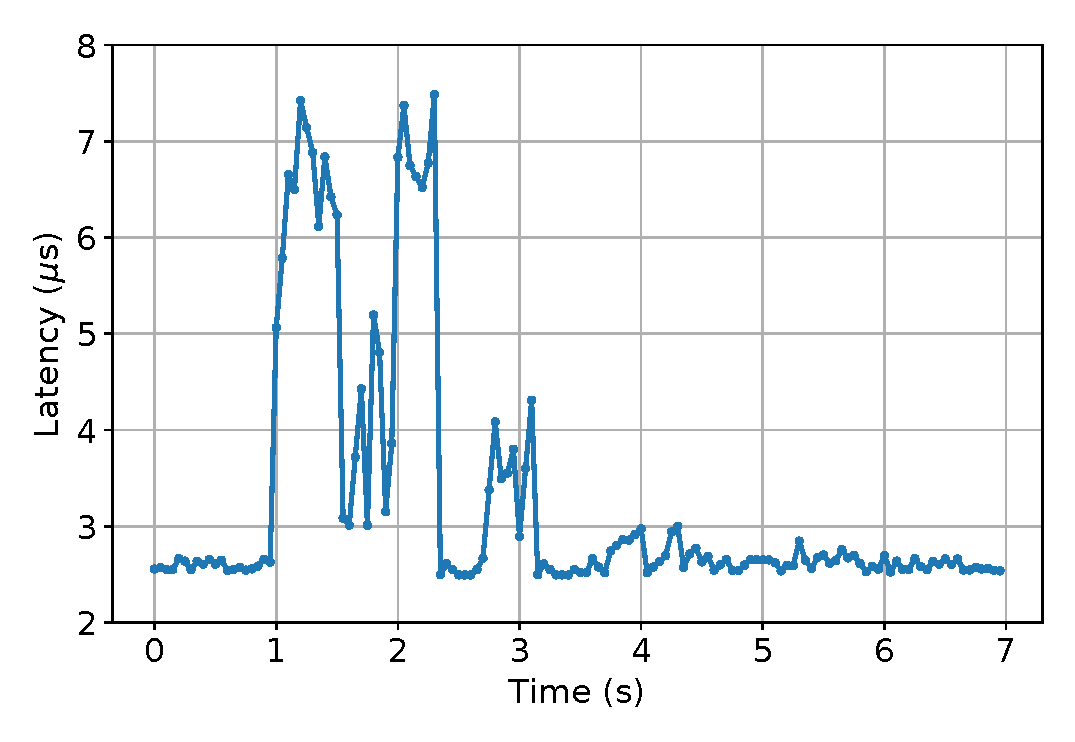
\includegraphics[width=0.8\columnwidth]{figure/aurelia/pcie-congestion.eps}  
    \caption{RDMA latency spikes almost 3 $\times$ by PCIe congestion.}
    \label{fig:pcie-congestion}        
\end{figure}

\noindent \textbf{Challenges: Flow control cannot prevent congestion.}
The point-to-point, credit-based flow control is focused on not overrunning the buffer only. 
%
It cannot deal with pairs of endpoints sharing a port on the switch because no information is exchanged between them. 


\noindent \textbf{PCIe congestion experiment.}
We design an experiment of multiple flows sharing a port on a switch and creating congestion.
%
Given no commercially available hardware for CXL, we use PCIe which shares the same flow control mechanism for our experiment. Interestingly, PCIe congestion has been identified and demonstrated under different setups~\cite{sbfc:ieee-micro:2005, pcie-congestion-model:sc:2016, invisible-probe:oaklnad:2021}. 

We create artificial PCIe congestion on a PCIe switch port shared by two devices. The machine uses a SuperMicro X11SPA-TF motherboard with a Broadcom PEX8747 PCIe switch. The PCIe switch has one upstream port to the CPU, and two downstream ports connecting to the devices, An Nvidia 2080 Ti GPU and a ConnectX-5 RDMA NIC connected to the PCIe switch.
%
\begin{figure}[ht!]  
    \centering
    %includegraphics[width=1\columnwidth, cframe=red!5!red 0.5mm]{figures/pcie-exp.eps}  
    \includegraphics[width=0.8\columnwidth]{figure/aurelia/pcie-exp.eps}  
    %\vspace{-2ex}
    \caption{Experimental setup for PCIe congestion.}
    \label{fig:pcie-experiment}        
\end{figure}
%
The PCIe switch connects with the host processor on one side and provides two ports connecting to GPU and RDMA NIC.
%
The experimental setup is shown in Figure~\ref{fig:pcie-experiment}.
%
During the experiment, the NIC periodically sends RDMA write requests to another machine every 100 microseconds. 
%
Each write request is sent from the CPU and travels through the PCIe switch to the NIC. 
%
After a second, a large integer array of 200 MB is moved from the main memory to the GPU. It causes heavy traffic on the upstream port and the downstream port to the GPU.
%
Their traffic collides on the upstream port of the PCIe switch %as they are both unaware of each other 
because flow control does not consider congestion that is caused by an outgoing link. 

We use PerfTest of Linux-RDMA library to measure the RDMA write request latency~\cite{ofed-perftest} shown in Figure~\ref{fig:pcie-congestion}. The latency spikes to almost 3x from 2.593 $\mu$s to 7.483 $\mu$s at the peak of PCIe congestion. 
%
PCIe's virtual channel is a feasible but not scalable solution because it provides only 7 channels. 
%
Traffic on the same channel still suffers from the same congestion as we have shown above. 
 
%\noindent \textbf{QoS Telemetry insufficiency.}
%QoS telemetry is still insufficient to address all potential congestion issues for the following reasons. 
%
%$First, QoS telemetry is focused on CXL.mem packets. 
%
\noindent \textbf{Challenge: Rate throttling between host CPU and devices only:}
CXL fabric offers a rate throttling mechanism called QoS Telemetry to avoid device overload and possible fabric congestion. 
%
The current QoS telemetry is designed specifically for CXL.mem between the host and devices with its local memory.
%
QoS telemetry allows memory devices to indicate their current internal load with 2 bits for CXL.mem response packets.  
%
The sender on the host CPU uses the reported internal load to monitor and throttle its request rate. 
%
However, not every sender on CXL fabric is on the host CPU. 
%
Peer-to-peer memory accesses using Unordered I/O in CXL.io support devices accessing the memory of another device directly. 
%
These peer-to-peer accesses under CXL.io are not throttled in the current design because QoS telemetry is only for CXL.mem and does not consider the sender to be other than a host CPU.
%
Machine learning and HPC applications illustrated in Figure~\ref{fig:cxl-topo} have evolved into heavy use of accelerators. 
Overlooking memory access from devices, especially accelerators, limits CXL fabric's ability to mitigate congestion and device overload.

%The rate throttling targets specifically for devices, mainly memory devices, that are associated with a host in the current design. 

%
% Perform rate throttling on CXL.mem packets alone cannot mitigate possible congestion because packets using the other protocols share the fabric.
%
%It is used for devices with its local memory including memory expansion devices and accelerators with device memory, e.g. GPU, FPGA, and ASIC.


%\TODO{merge this one with rate throttling}
%\noindent \textbf{Limit usage of load & congestion information}
%
%QoS telemetry does not consider peer-to-peer memory access packets on CXL.io protocols just introduced in the CXL 3.0 specification.
%

% \noindent \textbf{Challenge: Host controlled rate throttling}
% The request throttling of QoS telemetry is designed to be operated by the host.
% %
% It does not consider memory access can be initiated from devices, especially in a peer-to-peer fashion. 
% %
% These devices contain logic for a specific workload but do not have any general-purpose cores attached.
% %
% The current QoS telemetry design does not allow these accelerators to throttle themselves according to the device load. 
% %
% \stingw{I think we can still leave the rate throttling on host but it needs to be efficient like polling?}
% Moreover, a device performing peer-to-peer memory access depends on the host to throttle its request rate. 
% %
% %This contradicts the promise of resource disggreattion on a CXL fabric.
% This adds additional latency for throttling and thus risking more congestion on the fabric. 
%\stingw{we'll need additional hardware logic on CXL device that will initiate memory request}

\noindent \textbf{Challenge: Inaccurate load \& congestion information.}
QoS telemetry devises a mechanism called Egress Port Backpressure (EP Backpressure) to indicate the load of CXL switch ports.
%
It monitors the flow control backpressure situation on each CXL switch egress port. 
%
If the port cannot transmit packets due to insufficient credits, the port marks a 2-bit EP Backpressure value on the device load field of the outgoing request. 
% Omit the Temporary Throughput Reduction here
%
The overall load of a device is determined by the maxima of the device's internal load and EP Backpressure. 

However, the overall device load subsumes EP Backpressure, which is valuable congestion information. 
%
By taking the max value of the separated piece of information, QoS telemetry provides neither accurate device internal load nor congestion on the fabric.
%
The inaccurate information prevents QoS telemetry from performing end-to-end flow control and congestion control for the transport protocol.
%
The aforementioned challenges motivate us to design \aurelia. 
%
%\TODO{find place to say switch and CXL device are both nodes on a CXL}
\section{Design of \aurelia}
\label{aurelia:sec:design}
% \stingw{Reduce specific details on routing, merge multi-path and alternative routing. the design rationale is more important. we don't want to be tied to a 
% specific solution or design point.}

\begin{figure}[t!]    
    \centering
    \includegraphics[width=0.9\columnwidth]{figure/aurelia/cxl-fat-tree-routing-table.eps}
    \caption{CXL fabric as a Fat-tree using 12-bit FAN-ID address \emph{X:Y:Z}, which X, Y, and Z are hexadecimal values. Dash lines represent the routes from switch \emph{2:2:1}'s routing table.} 
    %representing \emph{pod:switch:device}}
    \label{fig:cxl-fabric-overview}
\end{figure}

We propose \aurelia, a network design involving devices and switches on CXL fabric. \aurelia provides addressing, routing, and congestion control protocol design by augmenting necessary functionalities on the fabric interface and switches.

\subsection{Addressing \& Flow}
%
\aurelia proposes to generalize CXL's port ID scheme to assign a 12-bit fabric node ID (FAN-ID) to a node that is either a device or a switch on the fabric. 
%
This is analogous to the 32-bit IP address describing hosts in an IP network.
%
%
FAN-ID assignment is agnostic to the underlying topology as long as a FAN-ID is unique for a node on a CXL fabric. 
%
\aurelia assigns FAN-ID to the physical interface of the device. It does not assign FAN-ID to logical interfaces sharing the same physical interface.
%
%\aurelia considers multi-tenancy a device-specific detail and do not provide additional FAN-ID to logical CXL interfaces
%Multi-tenancy of devices is out of the scope of this work.


With a similar analogy of "5-tuple" in the IP network, \aurelia defines a flow by a sequence of CXL packets that shares the same source device, destination device, protocol, and message classes.
%
Thus, routable CXL packets can be identified with a quadruple: \emph{(Source FAN-ID, Destination FAN-ID, CXL protocol, message classes)}. The CXL protocols include CXL.io, CXL.mem, and CXL.cache. The message classes are sub-type of packets within each protocol. For example, a CXL.mem packet writing to a device belongs to a class of \emph{M2S Request with Data} and a CXL.cache packet that carries responses from the device to the host belongs to a class of \emph{D2H Response with Data}.
%
Fat-tree with oversubscription is out of the scope of this preliminary study. 
%
For the rest of \aurelia's design, non-oversubscribed Fat-tree is assumed as the underlying topology. Different topology constructions and options are discussed in Sec.~\ref{sec:discussion}.
%

% \begin{comment}
% %FAN-ID 
% %because routing design can be based on per-node FAN-ID
% %each device usually has a single CXL interface with potentially different number of lanes. 

% Also, given the limit size of 12-bit address space, it is not efficient to assign multiple addressses to a single switch. 

% Per port address design like MAC address is not necessary
% because \aurelia's routing design is modeled after IP level routing on switches. 

% dragonfly's routing
% Minimal (MIN) : The minimal path is taken as described in
% Section 4.1.
% Valiant (VAL) [32] : Randomized non-minimal routing as
% described in Section 4.1.
% Universal Globally-Adaptive Load-balanced [29] (UGALG, UGAL-L) UGAL chooses between MIN and VAL on a
% packet-by-packet basis to load-balance the network. The
% choice is made by using queue length and hop count to estimate network delay and choosing the path with minimum
% delay. We implement two versions of UGAL.
% UGAL-L – uses local queue information at the current
% router node
% \end{comment}

% \begin{figure}[htb]
%     \centering
%     \includegraphics[width=\columnwidth]{figures/cxl-fat-tree-clear.eps}
%     \caption{\TODO{Routing example on Fat-tree.}} %representing \emph{pod:switch:device}}
%     \label{fig:fat-tree-routing}
% \end{figure}

\subsection{Routing}
\label{aurelia:sec:design:routing}
% P Path selection, R Routing itself, and L Load balancing. 
% Path selection determines which paths can be used for sending a given packet. Routing itself
% Routing answers a question on how the packet finds a way to its destination.
% Load balancing determines which path (out of identified alternatives) should be used for sending a packet to maximize performance and minimize congestion.
\aurelia routes packets based on FAN-ID addresses like IP routing.
%
CXL switches route a packet based on its routing table that maps a group of FAN-ID destinations onto a port. 
%
CXL switches transmit the packet out of a specific port to another switch that knows the next hop of this packet. 
%
The forwarding keeps on until the packet reaches the FAN-ID destination.

\noindent \textbf{Routing: Fat-tree as an example.}
%
Constructing a Fat-tree~\cite{fat-tree:sigcomm:2008} with 12-bit FAN-ID address shows a $k$-ary fat-tree with $k=4$ in Figure~\ref{fig:cxl-fabric-overview}.
%
Fat-tree uses a hierarchical scheme that assigns FAN-ID to nodes as \emph{pod:switch:device} with three segments.
%
Each segment is a 4-bit exact, hexadecimal value.  
%
For example, the leftmost CPU has FAN-ID \emph{2:0:2} representing it belongs to the third pod, the first switch, and the third node which is right after the switch itself.
%
Like IP routing, the routing on Fat-tree takes a single shortest path despite that the Fat-tree topology provides path diversity.
%
This creates bottlenecks even for trivial communication patterns because of the underutilization of available bandwidth.
%
Fat-tree implements a two-level routing table on each switch. One level of the table routes traffic down to the device and another one routes traffic toward the core of the fabric.
%
The table maps a set of destinations to a specific port. The routing lookup of destinations uses the address prefix for the traffic downward to the devices and the address suffix for the traffic going toward the cores.
%
The address suffix approach spreads traffic toward the fat-tree core across different switches based on FAN-ID.
%
The bottom of Figure~\ref{fig:cxl-fabric-overview} shows the routing table of CXL switch \emph{2:2:1} filled in gray. The prefix table routes packets toward its downstream switches \emph{2:0:1} and \emph{2:1:1}. The suffix table routes the packet upward to core switches \emph{4:1:1} and \emph{4:1:2}.  
%\TODO{add a running example on to Figure~\ref{fig:fat-tree-routing} or a new one.}
%

% \begin{comment}
% After identifying the quadruple, the existing knowledge of using flow as a major abstraction of load balancing and optimization becomes applicable for CXL fabric flow~\cite{FlowBender, Hedera, MicroTE}. In the case of multi-tenant devices, the quadruple cannot distinguish traffic between different tenants. Thus, per-packet load balancing schemes are more applicable for multi-tenant scenarios~\cite{Fastpass, DeTail, MPTCP}. 

% \weitao{Since we already assume next-generation connection, do we want to mention that the fat-tree topology can be a baseline, and we could further optimize the topology based on the application traffic pattern, like adding more number of lanes between frequently communicated devices.} 
% \stingw{I agree. topological optimization is a nice direction but it's hard to do it with current or near-future CXL technology. We can put it to the Discussion.}
% \stingw{We'll need CXL with higher radix to have more exotic topology, e.g. Dragonfly, Jellyfish, Xpander}

% \weitao{Active routing is another interesting type of routing. It is developed based on load-balancing routing. When one path is congested for a substantial amount of time, some flows will change the flow label to change the 5-tuple, so that the flow will pick a new path automatically. In your case, do you think you can also add a similar thing in "5-tuple" to make it "6-tuple" and enable active routing?} \stingw{introducing additional things on CXL's 256-byte packet is hard given the limited space. I don't agree with this one.}
% \end{comment}

% \TODO{we should talk about how the fabric manager will be implemented. GPU-SSD example is not a good one.}
% \reviwer{B: I encourage you to be more explicit about what's in/out of scope for the fabric manager}
%mirador:fast:2017, 
%uses multiple devices together~\cite{gullfoss:tech-report:2015, fractos:eurosys:2022}.
%
% \stingw{take out the GPU example!}
% The GPU-SSD example in Sec~\ref{sec:motivation:routing} is exactly one of these workloads.
% %
% The detouring of peer-to-peer memory access to an additional hop of memory buffer is not trivial to be specified as routing rules. 
% %
% The fabric manager first determines a fabric-attached memory device as the destination, then redirect the routing between the producer and the consumer devices to the memory device instead.  
% %
% The fabric manager then asks the consumer to read from the specific memory device instead of directly communicating with the producer.

\begin{figure}[ht!]
    \centering
    \includegraphics[width=0.9\columnwidth]{figure/aurelia/congestion-control-flow.pdf}
    \caption{\aurelia uses EP Backpressure notification to resolve congestions and overload signal for flow control to avoid overrunning the buffer on the device.}
    %has a congestion control loop for the fabric, a flow-control loop for the device.}
    \label{fig:congestion-control}
\end{figure}

\subsection{End-to-end Congestion Control}
\label{aurelia:sec:design:congestion-control}
% \stingw{More on pointing out the unique challenge, don't argue against delay based approach too much. Stay neutral before we have strong evidence.}
% \balance
% \begin{comment}
% These devices have shallow buffer space and different rate of producing/consuming data. %and are allocated with different bandwidth on the fabric.
% %
% With strictly peer-to-peer communication, the producer matches consumer's rate to not overwhelm the consumer. 
% %
% The slow-down on faster producer leads to under-utilization of the device. 
% %
% To improve resource utilization, fabric attached memory pool can serve as the buffer and an alternative routing destination between devices. 
% %
% This decouples the producer and the consumer and allows faster producer to be utilized by other workload.
% %
% The switch identifies CXL.io packets performing peer-to-peer memory access, and notifies the fabric manager when it sees EP Backpressure on its port with CXL.io.
% %
% The fabric manager modifies the routing table between the producer and consumer, and routes the packets to a specific fabric attached memory pool attached to the either side of the CXL switch. 
% %
% The fabric manager then asks the consumer to read from the specific fabric attached memory pool instead of directly communicating with the producer.

% \weitao{One suggestion about the signals: the internal load and the EP backpressure could be represented in a uniform format. Both of them suggest the congestion level, but for end-point devices and switches respectively.}\stingw{this sounds about right!}

% \weitao{Another wild idea is that, if switches and end-point devices could provide more quantitative signals (like 8 bits) to represent congestion level, rather than a single bit to provide a binary signal about congestion, the performance of the congestion control algorithms could be largely improved. As a supporting fact, many commodity switches can support reporting and piggybacking telemetry information for each packet, including per-hop queueing delay and per-hop utilization.}\stingw{the problem with CXL is the packet is 256-byte. we could argue for using more bits in the discussion section. I tried to do the minimal modification to CXL to achieve something useful.}    
% \end{comment}
\noindent \textbf{Extending existing mechanisms.}
%
\aurelia implements end-to-end congestion control with overload avoidance by extending existing mechanisms of CXL. 
%
The mechanisms are EP Backpressure on switches, internal load reported on receiving devices, and rate throttling on the sending devices.
%
%EP Backpressure and ECN both indicate congestion explicitly to the receiving endpoints.  
%and need packets to convoy the congestion signal back to the sender.
%
EP Backpressure triggers switches to mark packets on their way to the receiving device when noticeable queuing is on the switch.  
%
This is similar to Explicit Congestion Notification (ECN) for Ethernet and Infiniband because they react when the queuing situation starts to indicate congestion.
%
Internal load reporting triggers an overloading signal when the device is overloaded. 
%
Device overload is likely to cause significant device-side delay or even loss of CXL packets.
%
\aurelia, unlike CXL's design, separates EP Backpressure and the device's internal load as they represent fabric and device information. 
%
% for congestion control and overload avoidance 
% EP Backpressure and internal load use 1 bit for each on the packet header. 
%
Rate throttling controls the sending rate into the fabric to avoids congestion and overload. 
%
%On top of these mechanisms, CXL fabric is a lossless fabric by its point-to-point flow control design.
%
% These factors determine \aurelia to implement a rate-based congestion control with overload avoidance for the devices. 

\noindent \textbf{Algorithm.}
\aurelia's congestion control algorithm operates on the switch, the receiving device, and the sending device.
%
On the switches, they mark the packets when the ratio of EP Backpressuring events in its recent window is larger than a specific threshold.
%
On the receiving devices, they piggyback an overloading signal to the sending device when its sending rate exceeds the receiver's processing rate.
%
The receiving device notifies the sender with EP Backpressure notification (EPN) on its response to the sending device when it receives EP Backpressure marked packets.  
%
On the sender side, the sending devices throttle the sending rate based on the 1-bit signal of EPN and the 1-bit overloading signal. 
%
When the sender receives a response packet marked with EPN or an overloading signal, the sender records its current rate $R_{c}$ as the target rate $R_{t}$ for later recovery and cuts its rate half in default. 
%
The rate cut can also be determined by also a rate reduction factor $\alpha$ like DCTCP and DCQCN~\cite{dcqcn:sigcomm:2015}.         
%
The recovery of reduced sending rate has two different paths depending on the trigger.
%
If the reduction is triggered by EPN, then the recovery to the target rate $R_{t}$ is expected in a fixed number of iterations. 
%  
If the reduction is triggered by an overloading signal, then the recovery is an additive increase.

% \stingw{fast recovery for EP Backpressure and slower recovery, i.e. additive, for internal load}
%
% \stingw{EP Backpressure and internal load use 1 bit for each on the packet header.}

%Flow control preventing buffer-overrun is handled by the link and physical layer of CXL and thus not a concern for the transport layer. 

\noindent \textbf{Protocol implementation.}
\aurelia relies on hardware implementation to throttle sending rate for congestion control due to sub-$\mu$s latency and peer-to-peer memory access requirements.
%
First, rate throttling has a tight latency requirement of sub-$\mu$s on CXL fabric.
%
Pond measured end-to-end CXL.mem latency and obtained latency ranging to 270 ns on CXL system with a single switch~\cite{cxl:hoti:2022, pond:asplos:2023}. 
%
Under the same assumption, the latency of CXL packet traveling through a two-level fat-tree takes around 680 ns that is under 1 $\mu$s.
%
Second, peer-to-peer memory access between devices is expected, especially with the usage of accelerators. Therefore, \aurelia extending CXL's original design generalizes the reporting of device load for all kinds of memory access, including peer-to-peer memory access between devices.
%
Peer-to-peer memory access between devices without additional embedded CPU motivates the necessity of implementing rate throttling in hardware on the CXL interface. 
%
The control plane of these hardware devices is kept on the host CPU, but the execution of rate throttling is on hardware to meet these requirements.  
%
Hardware-based rate throttling ensures all devices on the CXL fabric are able to control their sending rate and further reduces the congestion and overload.
%
Implementing rate throttling logic on hardware has been used on RDMA over Infiniband and Ethernet with RoCEv2 support and thus suggesting the feasibility in the case of CXL fabric. 

\noindent \textbf{Comparable protocol design on lossless fabric.}
\aurelia's congestion control design is inspired by congestion control on existing lossless fabric, such as Infiniband and DCQCN for RoCEv2, implemented a rate-based congestion control algorithm requiring Explicit Congestion Notification (ECN) on switch to indicate congestion.
%
Infiniband switches mark packets with a Forward ECN (FECN) bit when congestion is detected~\cite{infiniband-spec}. 
%
The receiver receives the FECN-marked packets and sends a Backward ECN (BECN) marked packet to the sender.
% 
The sender throttles its injection rate when it gets packets with BECN. The throttling over time reduces congestion and the fabric returns to a state without any congestion. 
%
Thee FECN marking of packets requires switch support and the implementation of BECN and rate throttling requires additional logic in CXL interface hardware.
%
DCQCN, a congestion control protocol designed for RoCEv2, relies on the ECN of Ethernet to notify the sender to adjust its injection rate similar to Infiniband~\cite{dcqcn:sigcomm:2015}.
%
% Before throttling, \aurelia sets the rate as the target rate for later recovery.
% %
% \aurelia throttles the rate of the sender, when the receiver notifies it of the congestion signal and generates EP Backpressure. 
% %
% After rate throttling, \aurelia enters the recovery phase and then performs additive increase when approaching the target rate~\cite{dcqcn:sigcomm:2015}. 
\subsection{Advanced Routing}
\label{aurelia:sec:design:advanced-routing}
\noindent \textbf{Multi-path routing.}
%
The two-level routing table of Fat-tree is just an implementation of multi-path routing together with a specific topology. \aurelia imposes no restriction on how the fabric should be constructed. Instead, \aurelia requires routing tables to be able to map a destination to multiple next-hop FAN-ID and its corresponding metric. The metric can be distances in terms of hops or local congestion level on each switch port. 
%
\aurelia selects a next-hop with minimal metric and randomly selects one if there are multiple next-hop options with equal metric.  
%
Considering the number of hops for shortest path routing, \aurelia can perform a random selection for the next hop on flow granularity or on packet granularity. The former is similar to Equal-Cost Multipathing (ECMP) and the latter is similar to packet spraying. 

\noindent \textbf{Adaptive routing.}
%
ECMP and packet spraying are oblivious to the workload. 
%
\aurelia would be able to further exploit local per-port information on the switches or the fabric manager manipulating the routing table to achieve adaptive routing.
%
\aurelia uses per-port EP Backpressure as a measure of local congestion indication. 
%
For selecting an egress port with minimal congestion on the switch, \aurelia uses power-of-2 choice~\cite{power-of-two:tpds:2001} to avoid congestion on ports based on possibly delayed congestion information.
%
Additionally, \aurelia allows the fabric manager to insert routes and has the sole authority to modify the routing table at any time.
%
This is useful for the workload that requires non-trivial routes tailored to specific workloads~\cite{gullfoss:tech-report:2015, fractos:eurosys:2022}. 


\section{Evaluation of \aurelia's Design}
\label{aurelia:sec:eval}
%
We simulate the design of \aurelia because CXL hardware supporting CXL 3.0 with fabric is not available to the author at the time of writing.
%
We evaluate \aurelia's congestion control design using routing described in Sec.~\ref{aurelia:sec:design:routing}. 
%
Additional routing designs, such as multipath and adaptive routing, are not enabled for the evaluation.
%
The evaluated workloads are: (1) key-value store on memory expansion modules~\cite{samsung-memory-expander:hcs:2022}, and (2) machine learning model inference on GPUs/accelerators involving collective communication~\cite{aws-inferentia:2019}.
%
They represent different usage of CXL fabric: one is focused on CPU and memory expansion while the other is focused on the data exchange between accelerators.
%
The baseline of the evaluation is vanilla CXL described in its specification~\cite{cxl-3-0-spec}.
%
It performs point-to-point flow control for packets of each CXL protocol.
%
It does not employ any end-to-end congestion control or flow control mechanisms.
%
% \stingw{It has limited support for dev load reporting for CXL.mem
% but it does not consider the fabric situation.}

% \TODO{Define the baseline here please.}
% \stingw{
% What are we comparing to?
% %
% CXL default with only PCIe flow control.
% %
% Make sure the large flows don't shut down the port if flows collides.
% }
%\stingw{The issue with PCIe is that all traffic are fighting together. CXL-base has different protocol and message classes}  

\subsection{Packet-level Simulation using ns-3}
\label{aurelia:sec:eval:ns3-simulation}
We use NS3~\cite{ns-3} to simulate packet level behavior on a CXL fabric.
%  
NS3 is a discrete-event network simulator that is open-sourced and well-established in the research community. 
%
Our implementation uses primitive, built-in NS3 classes and starts from scratch because there is no existing simulator for CXL fabric. 
%
Previous simulators of other lossless fabrics are focused on RDMA over Converged Ethernet (RoCE)~\cite{dcqcn:sigcomm:2015, hpcc:sigcomm:2019,pint:sigcomm:2020}.
%
These implementations are not usable for CXL fabrics because they assume the usage of Ethernet, IP, and the RDMA interface cards.
%
CXL fabrics assumes none of those as the devices on the fabric issue load/store instructions directly.   
%
%The difference between our simulation and the latencies reported on the CXL expansion chassis is within 5\%.

The hardware parameters are cross-checked with published literature~\cite{pond:asplos:2023, demystifying-cxl:micro:2023, h3platform-cxl-memory}. 
%
The latencies on each hardware component are calibrated with H3 platform's CXL expansion chassis supporting CXL 2.0~\cite{h3platform-cxl-memory}. 
%
The chassis integrates a CXL switch~\cite{xconn-cxl2-switch} supporting CXL.mem and CXL.io that are used in the evaluation.

We simulate CXL's transaction layer and link layer in 256B mode assuming a PCIe 6.0 physical layer.
%with its forward error correction are fully controlled by the hardware.     
%
The physical layer of PCIe 6.0 with 256 GB/s is on a 16-lane configuration. 
%
All links in the simulation use this configuration.
%
All messages classes of CXL.mem and CXL.cache are supported.  
%
CXL.io functionalities for peer-to-peer memory access are supported. 
%
Packing of CXL.mem and CXL.cache messages are implemented to ensure the number of packets on the fabric are accurate to the specification.

The simulator enables multi-level switching and implements \aurelia's addressing, routing, and congestion control mechanism on top of CXL's port-based routing.
%
There are 16 nodes on a 2-level fat-tree topology. 
%
In the case of machine learning model inference, the topology connects 8 accelerators and 8 memory expansion devices.
%
In the case of key-value store, the topology connects 12 memory expansion devices with 4 CPUs.
  
%
\subsection{Simulation of Large Model Inference}
\label{aurelia:sec:eval:inf}
%
We study the improvement of inference throughput on LLaMA2 70B model~\cite{llama:arxiv:2023} due to improved congestion control on the CXL fabric.
%
The inference of the model operates on the unit of tokens for a sequence of input and output data.
%
First, the fabric connects the accelerators to the memory expansion devices that store the model weights.
%
Partial weights of the model are kept on the accelerator as the weights are loaded partition by partition.  
%from the memory expansion devices.
%
Each accelerator stores 8.125 GB partition on the device and another partition on the memory expansion devices.
% The weight loading and inference exec are pipeline parallel.
%
This leaves enough capacity for intermediate generated tokens on the accelerators.
%
A run of inference performs 2 operations of weight loading operations between the accelerators and the memory expansion devices.
%
Second, the fabric supports the communication among accelerators that aggregates tokens.
%
A run of inference performs 2 operations of all-reduce collective communication among the accelerators to aggregate the intermediate and the output tokens.
%
Each all-reduce operation exchanges 810 $\times$ 8 MB of data among the accelerators.
%
The all-reduce operations are 3 milliseconds apart as these durations represent the computational part of the inference run.
%
The simulation executes 1000 runs of inference based on the aforementioned parameters.  
%
\aurelia's improved congestion control aims to speed up both the weight loading and the all-reduce operations.
%
% The 3 milliseconds durations corresponds to the two major components of the LLaMA2 model, self-attention and feedforward layers.    
% These tokens are an $E$-dimensional vector, where $E$ is 16384 in our setup.
% %
% A sequence has up to $L$ tokens, where $L$ is 256 in our setup.
% %
% A run of inference processes $B$ $L$-token sequences containing $E$-dimensional vectors, where $B$ is the batch size of 2048 in our setup.

\aurelia achieves 11\% improvement on median throughput and 17\% improvement on the 10th percentile throughput because of faster weight loading and all-reduce operations. 
%
These operations encounter 2.1$\times$ fewer times of pause on the links than the baseline when the links are out of credits to send packets.
%
EPN of \aurelia throttles the sending rate to avoid triggering the pause on links. 
%that the sender and switches do not have enough credits to progress.
%
The traffic pattern of weight loading and all-reduce operations does not impose much imbalance therefore there is no overload on any of the accelerators that needs the overload signal for remediation.
%
Imbalanced traffic among accelerators could test \aurelia's effectiveness on such kind of traffic pattern. 
%
We leave it for future investigation.

\subsection{Simulation Results on YCSB Benchmarks}
\label{aurelia:sec:eval:kv-store}
%\TODO{Using A, B, C, and F results with ns-3 simulation}
%
We study the 99th percentile latency on key-value stores using YCSB benchmarks \cite{ycsb:socc:2010}.
%
YCSB benchmarks are widely used to evaluate key-value stores with a mix of insert, read, and updates operations.
%
They are used to evaluating key-value stores in memory or on SSD.
%
In the case of CXL fabric, we evaluate key-value stores on fabric-attached memory expansion.
%
Memory expansion devices manage their own coherence between themselves and connected CPUs.
%
They invalidate data on CPU cache to maintain the coherency.

%\stingw{why scan operations are not doable in our setup, so we only do A, B, C and F.}
We evaluate YCSB A, B, C, and F for read, write, and read-modify-write operations on the key-value store.
% insert is weak here. 
%
YCSB D and E are not evaluated because both of their performance depends on the recent accessed keys and also how the keys are hashed when inserted. 
%
These additional requirements make them not ideal for us to objectively evaluate the improvement provided by \aurelia.
%
YCSB A, B, C, and F, on the other hand, access key-value pairs based on a fixed Zipf distribution.
%
Zipf distribution makes the probability of accessing $n^{th}$ key inversely proportional to $n$.
%
The plot of a Zipf distribution in linear scale is similar to an exponential decay curves so the first few $n^{th}$ keys are way more likely to be frequently accessed.
%
This makes the traffic imbalanced because the requests to a key-value pair are more likely to be headed to a certain memory expansion device. 

% \stingw{
% %For D: Request distribution: latest, E needs scanning for a range. 
% For D, it needs an assumption of the latest and assumes inserts are hashed. 
% Therefore, its performance depends on the hash for the "latest" distribution.
% %
% For E, scanning also depends on the hash for insert. 
% %
% This hash heavily impacts how the performance will be looked like and it's not a fixed distribution like Zipf we can control. 
% }

\aurelia's improvement on 99th percentile latency for YCSB benchmarks is shown in Figure.~\ref{fig:cxl-ycsb-results}.
%
\aurelia's EPN and overload signal combined handles the imbalance of traffic caused by Zipf distribution. 
%
The improvement for read-only YCSB C is the lowest because it incurs a request-response pair to a specific memory expansion device without any cache invalidation.
%
The improvement for YCSB A and B is higher because YCSB A and B incur write and subsequently cache invalidation from the memory expansion device to other CPUs.
%
The improvement of YCSB A is higher than YCSB B because it has 50\% of operations as writes compared to 5\% of YCSB B.  
%
EPN has a higher contribution to the latency improvement because overload signal makes  
22\% more improvement on YCSB F compared to \aurelia without it.
%
This is expected as overload shouldn't be a frequent event or memory capacity and bandwidth are not properly provisioned.
%
In average, \aurelia without overload signal is only 14\% worse on all YCSB benchmarks.

% \stingw{The explanation: EPN handles the congestion and overload signal in this case does contribute to it.
% %
% But I guess the question is about the ratio? 
% %
% 22\% more on YCSB F compared to \aurelia without it. In average, 14\% more on all.
% }
%
%\TODO{A figure for 99th percentile latency on YCSB A, B, C and F.}

\begin{figure}[ht!]    
    \centering
    \includegraphics[width=0.9\columnwidth]{figure/aurelia/ycsb.pdf}
    \caption{YCSB benchmarks with higher ratio of writes demonstrate more improvement.} 
    \label{fig:cxl-ycsb-results}
\end{figure}


%\section{Additional Fabric Enhancement Consideration}
\section{Discussion}
\label{aurelia:sec:discussion}
%\TODO{extending discussion for 6-page HotNets}
% \noindent \textbf{The scale and economic of CXL fabric}
% how large should we scale CXL fabric to be still cost-effective~\cite{pond:asplos:2023}?
% Pond dem
\noindent \textbf{Alternatives: NVLink and PCIe fabric.}
%\TODO{Clean up the text here!}
% \stingw{Here to add NVLink + GH-200 discussion. 
% NVLink is propriety and has a narrower usage even with GH-200.
% GH-200 with NVLink is at most a CXL type-2 usage.
% }
%\stingw{All these alternatives are not designed to be as general as CXL}
%
% Alternative interconnects are designed for specific use cases, and they lack of the generality of CXL. 
% 
NVLink is an interconnect by Nvidia for high throughput between GPUs~\cite{nvlink}. NVLink supports GPU-CPU interconnect with cache coherency on the recent Grace-Hopper 200 hardware~\cite{dgx-gh200}. 
%
NVLink presents an interesting alternative to CXL but has three limitations. 
%
First, NVLink with its cache coherent extension in fact supports GPUs as CXL type 2 devices. However, it does not support CXL type 3 devices that expand memory independent of the main memory capacity. The capability to scale memory capacity is attractive for memory-hungry large language models~\cite{gpt3:neurips:2020,llama:arxiv:2023}. 
%%NVLink with its cache coherent extension presents an alternative of CXL Type2 interconnect.   
%
Second, NVLink scales to 256 endpoints though connects only GPUs as endpoints~\cite{dgx-superpod}. 
%\stingw{Third, NVLink itself does not scale beyond 8 or 16 GPUs on a server.}
Third, NVLink as a propriety interconnect limits its usage beyond Nvidia's hardware.
%
PCIe using Non-Transparent Bridge (NTB) expands beyond a single root complex to multiple hosts as a fabric with many more connected devices~\cite{pcie-spec}. 
%
%PCIe transactions mapped to NTB’s specific memory range are forwarded
%with address translation to the destination host.   
%
% Using NTB with a shared address space spanning all hosts and their devices enables devices to directly communicate with point-to-point DMA over PCIe fabric~\cite{gigaio-fabrex}.
%
However, PCIe, included in CXL as CXL.io, lacks the memory and caching semantics that are much needed in the face of accelerator and memory expansion. 
%
This is exactly the reason that motivates the creation of CXL.
%
Both NVLink and PCIe fabric show a fabric supporting a subset of CXL's use cases but not all of it.    
%
%\stingw{why not hooking Ethernet directly to each device?}

\noindent \textbf{Co-existence of CXL and Ethernet.}
Given the scaling discussion, CXL is still unlikely to completely replace Ethernet in the datacenter due to its current PCIe based physical layer design. 
%
We speculate CXL fabric is beneficial on rack-scale because of the signal integrity and CXL switch hardware cost. 
%
CXL fabric is not intended to replace existing Ethernet completely but as a cost-effective alternative on the rack level. 
%
CXL packets are converted to Ethernet frames at a location equivalent to a top-of-rack switch for cross-rack traffic.
%
Previous work investigating the co-existence of Ethernet and a memory fabric follows a similar approach~\cite{aquila:nsdi:2022}.

%\stingw{Interconnect comparison: NVLink + C2C, other inter core interconnect, PCIe, CXL}
\noindent \textbf{Cost-effective scales of CXL fabric:}
%\noindent \textbf{Co-existence of CXL and Ethernet.}
% \stingw{how large should we scale CXL fabric to be still cost-effective~\cite{pond:asplos:2023}?}
%
CXL is an exciting technology but it comes with its limitations.
%
First, CXL requires retimer to maintain its signal integrity after 500 mm distance~\cite{microchip-cxl-retimer,asteralabs-pcie-retimer}. The retimer raises the hardware cost and incurs extra 20 ns latency every 500 ~\cite{pond:asplos:2023}.
%
Second, to scale CXL supporting multi-level switching, multiple CXL switches are used. They cause an estimated 70 ns latency for each hop over a switch.
%
Considering the combined cost of switches, retimers and additional memory controllers, Pond~\cite{pond-saving:ieee-micro:2023} suggests a
scale smaller than 32-socket for their memory expansion usage (Shown in Figure~\ref{fig:kvs-cxl}).
%
However, the exact scale of cost-effective CXL fabric for model training and HPC usage (Shown in Figure~\ref{fig:ml-acc-cxl}) remains to be determined in future works. 
%
%Pond also suggests the exact scale of a cost-effective CXL fabric depends highly on the workload, e.g. Pond's memory expansion usage for VM on public cloud.

% \stingw{CXL is not a solution for everything. It has signal integrity limits that making it scale beyond not cost-effective and with bloated latency by these intermediate retimers and switches.}
%
% \stingw{Pond suggest 8-socket for the use case is shown as Figure 1-(b). Pond also said that the exact scale depends on the workload. If the workload can tolerate higher latency or has a clear and predictable memory access pattern, then the scale of CXL can be larger if it's cost-effective.}
%    

\noindent \textbf{Topologies and multipathing.}
The flexible topology of CXL fabric empowers the fabric operator to optimize their topology based on the traffic pattern. 
%
The to-be-released CXL 3.1 will support native multipathing. Topologies with high path diversity such as Dragonfly can be easily implemented with CXL's multipathing. 
%
Packet spraying and ECMP on Fat-tree related topologies can be benefited from this as well.
%
With CXL switch prototype supporting 32-port ~\cite{xconn-cxl2-switch}, we expect these higher radix switches to enable us to explore different design options.
%
For example, the fabric operator can assign a high over-subscription ratio if the traffic pattern demonstrates high localities under a CXL switch. 
%
As another example, the fabric operator can add or reduce the bandwidth of certain CXL to better match the bandwidth to the actual demand between particular nodes. 

\noindent \textbf{Security implication: Delay based side channel.}
CXL fabric exposes the server interconnect to a shared fabric that may contain malicious devices.
%
The fabric exposes a delay-based side channel caused by interconnect congestion.
%
This side channel enables attackers to recover information from different delay patterns. 
%
Previous works~\cite{invisible-probe:oaklnad:2021} investigate the same issue with PCIe on a server. 
%
CXL fabric enlarges the attack interface by leaving all devices vulnerable to delay probing.
%
Delay probing requires accurate timing measurement.
%
CXL's usage of direct load/store makes it easy for attacker to acquire accurate timing of every memory load/store. 
%
Defense against this specific type of side channel attack is interesting for future security research. 
%
% [23] M. Kurth, B. Gras, D. Andriesse, C. Giuffrida, H. Bos, and K. Razavi, “Netcat: Practical cache attacks from the network,” in Proceedings of IEEE Security & Privacy 2020. IEEE, 2020.
% [24] S.-Y. Tsai, M. Payer, and Y. Zhang, “Pythia: remote oracles for the masses,” in 28th USENIX Security Symposium (USENIX Security 19), 2019,
% Irazoqui et al. also conducted cross-CPU attacks on the CPU interconnect [89]

% \noindent \textbf{Topologies and multipathing with CXL 3.1.}
% The to-be-released CXL 3.1 will support native multipathing. Topologies with high path diversity such as Dragonfly~\cite{} can be easily implemented with CXL's multipathing. 
% %
% Packet spraying and ECMP on Fat-tree related topologies can be benefited from this as well.
%
% \stingw{Yes CXL 3.1 is pending to have native multi-path support. But how could that be useful? it could be useful for dragonfly that is useful for HPC communication patterns. 
% cite "High-Performance Routing with Multipathing and Path Diversity in Supercomputers and Data Centers" for their non-minimal multipath
%
% It could be another way to implement 
% 5. higher radix -> different topology dragonfly  % -> VLB in the case direct connected topology 
%}

% \begin{comment}
% The biggest challenge and our focus in building LegoOS is the separation of processor and memory and
% their management. Modern processors and OSes assume
% all hardware memory units including main memory, page
% tables, and TLB are local. Simply moving all memory
% hardware and memory management software to across
% the network will not work
% \end{comment}

% \noindent \textbf{Interconnect Integration.}
% %
% %PCIe, as the wildly adopted option, supports fabric switching for expandability as an ideal interconnect. 
% %
% %The limitation of PCIe is that a single fabric can only have a single root except when using Non-Transparent Bridge (NTB).
% %
% PCIe's Non-Transparent Bridge (NTB) enables PCIe to expand to multiple hosts with more than one PCIe root complex. 
% %
% %NTB is not a bridge but an end-point device with its PCIe BAR address range. 
% %
% Operations mapped to NTB's specific memory range are forwarded with address translation
% %through the NTB along with address translation as the other host uses a different address space
% ~\cite{hou:hpca:2013,smartio:tocs:2021}. 
% %
% %The address translation of NTB can be further integrated into a PCIe fabric switch.
% %
% Using a shared address space across all devices 
% %with address translation 
% enables devices to directly communicate with point-to-point DMA over PCIe fabric~\cite{gigaio-pcie-swtich}.
% %
% CXL 3.0 introduces fabric switching 
% %and further cache coherency 
% to connect racks of devices and accelerators~\cite{cxl-3-0-spec}. This allows CXL to seamlessly connect accelerators on different servers.    
% %
% DUA~\cite{dua:nsdi:2019} provides an overlay fabric on top of the existing physical communication stacks, e.g., PCIe, Ethernet, DDR, etc.



% \stingw{fabric is exposed instead of having a confined interconnect. do we have higher risk of getting side channel attack and other secruity risks?}
% \begin{enumerate}                
%     \item how large should we scale CXL fabric to be still cost-effective~\cite{pond:asplos:2023}.    
%     -> CXL offers higher bandwidth than Ethernet as accelerators drive large throughput
%     -> it doesn't need the PCIe-Ethernet conversion through NIC. cutting cost and removing potential bottleneck.
%     \item What's the use of Ethernet and its compatibility CXL fabric in datacenter~\cite{aquila:nsdi:2022}. 
%     -> Swtich deisgn can be discussed like Aquila's TiN.    
%     \item Swapping fat-tree direct-connected tooplogy like Dragonfly if we have higher radix switches. memory access latency advantage shown in~\cite{aquila:nsdi:2022}. 
%     \item Native support of collective operations, it'll be useful for accelertator and HPC.
%     \item Programmability
%     a. we have programmable dataplane on the regular network for processing on the packets that needs to happen on the line rate
%     b. can we reproduce that here? 
%     c. possible use cases: load balancing, fine grain memory protection, data manipulation  
%     \item some security~\cite{invisible-probe:oaklnad:2021}
%     %\item Fat-tree with oversubscription % is out of the scope of this preliminary study.
%     %\item software stack compatibility?    
%     %\item multi-casting

%     %\item traffic pattern of memory and cache invalidation is pretty unknown
%     %\item accelerators are everywhere, what's the benefit of sticking them onto CXL fabric?
%     %\item other abstraction other than active network that still makes sense?
%     %\item memory fabric or a general purpose rack-scale fabric
% \end{enumerate}

%CXL controlled random graph -> optimization graph workload  

% \begin{comment}
% cite Understanding Host Interconnect Congestion?

% CXL-fabric+
% 1. deadlock avoidance
% 2. Native support of collective operations, it'll be useful for accelertator and HPC. (multi-casting)
% 3. Programmability
%     a. we have programmable dataplane on the regular network for processing on the packets that needs to happen on the line rate
%     b. can we reproduce that here? 
%     c. possible use cases: load balancing, fine grain memory protection, data manipulation  
% 4. Monitoring
% 5. higher radix -> different topology dragonfly  % -> VLB in the case direct connected topology 
% cite "High-Performance Routing with Multipathing and Path Diversity in Supercomputers and Data Centers" for their non-minimal multipath
% \end{comment}

%
% 1. CXL can have any topology, what kind of topology can provide good multi-path with low cost?
% Multiple paths can be found on Dragonfly in ~\cite{aquila:nsdi:2022} and some other HPC used topology.
% %
% 2. Dragonfly tried to reduce long optical links to save cost. The same rationale actually applies to CXL fabric too.
% This is because CXL is based on PCIe physical layer, long links can be problematic as it’ll need additional retimers or redrivers to improve signal integrity. These retimers or redrivers will drive up latency and most importantly cost of CXL deployment.
% %
% 3. Clos-topology (indirect) has many hops and longer cables which may need  retimers or redrivers too.
% %
% 4. so prefer direct topology like Dragonfly (at least for now). This remains room for optimization.

% \stingw{any topology variant that is more tailor-made to CXL fabric's workload characteristics? 
%     -> high radix or low radix CXL switch in the future?}

\section{Conclusion}
\label{aurelia:sec:conclusion}
%
Emerging standard CXL facilitates disaggregation with the support of multi-level switching. 
%
However, the current CXL fabric presents scalability and latency limitations. \aurelia addresses the challenges by designing proper addressing, routing, and transport layer design.

\section{Sources for Material Presented in This Chapter}
Chapter~\ref{aurelia:chap}, in part, reprints material as it appears in a published paper titled: 
"Aurelia: CXL Fabric with Tentacle" by Shu-Ting Wang and Weitao Wang~\cite{aurelia:words:2023}. 
%
The dissertation author was the primary researcher and author of this material.
\chapter{Conclusion}
\label{conclusion:chap}
%
The dissertation investigates the redundant communication between servers for large-scale web and cache requests and redundant data movement between accelerators for compute-intensive applications.
%
The redundancy is an impending and critical issue for datacenters designed for hardware accelerators and disaggregated resources.
% 
The dissertation makes the following three contributions to address this.


The first contribution of the dissertation is \daronpon. 
%
\daronpon is a datacenter-wide, inter-rack distributed load-balancing system for replicated datacenter services.  
%
\daronpon, at its heart, is a highly efficient gossip protocol that ensures that requests originating at any point in the datacenter can be directed away from overloaded replicas at sub-RTT timescales.
%
Through a mixture of simulation and deployment within AWS's cloud network, we show that \daronpon reduces the 99th percentile of latency for common workloads by up to 2$\times$ while admitting 10\% more requests per unit time. 

The second contribution of the dissertation is \dmx. 
%
\dmx acts as a compute-enabled bypass for inter-accelerator communication. 
%
The data restructuring and communication overhead of executing a single application using a chain of accelerators is defined as the data motion overhead.
%
With the current paradigm of using accelerators, the data motion overhead is very likely to outweigh the benefits from all these chained heterogeneous accelerators.
%
In contrast to previous works on accelerators that deal with accelerating only compute kernels, \dmx focuses on accelerating data motion within a chain of heterogeneous accelerators in a multi-accelerator datacenter.
%
To that end, \dmx reduces data movement, accelerates data restructuring, and enables interoperability between heterogeneous accelerators from different domains through a cross-stack hardware-software solution. 
%
The results from five end-to-end applications show that utilizing \dmx offers up to 8.2$\times$, 13.6$\times$, and 5.2$\times$ improvement in latency, throughput, and energy efficiency in a multi-accelerator system, respectively.

The third contribution of the dissertation is \aurelia. 
%%%%%
\aurelia leverages the emerging interconnect of CXL to investigate the design of a scalable fabric for accelerators and fabric-attached memory expansion.
%
Compute Express Link (CXL) has emerged as a frontier for disaggregation by providing a fabric supporting memory accessing, caching, and peer-to-peer memory access between devices.
%
CXL externalizes the internal memory fabric of a server and blurs the notion of server for realistic disaggregation.
%
The key feature of enabling CXL as a memory fabric is its support of multi-level switching up to 4096 endpoints.
%
However, CXL's current multi-level switching poses challenges on scalability and latency. 
%
To cope with the expected scale of CXL fabric and take full advantage of disaggregation, we propose \aurelia.
%
\aurelia architects addressing, routing, and transport as networking layers, which are typical in host networking, for CXL fabric.
%
\aurelia uses existing CXL mechanisms to realize the much-needed functionalities for a scalable fabric.
%
With these networking layers, \aurelia improves by 27\% on throughput for large language model inference and up to 2.6 $\times$ for key-value stores on YCSB benchmarks.

% \chapter{Just a Test}
% This is only a test.
% \section{A section}
% Lorem ipsum dolor sit amet, consectetuer adipiscing elit. Nulla odio
% sem, bibendum ut, aliquam ac, facilisis id, tellus. Nam posuere pede
% sit amet ipsum. Etiam dolor. In sodales eros quis pede.  Quisque sed
% nulla et ligula vulputate lacinia. In venenatis, ligula id semper
% feugiat, ligula odio adipiscing libero, eget mollis nunc erat id orci.
% Nullam ante dolor, rutrum eget, vestibulum euismod, pulvinar at, nibh.
% In sapien. Quisque ut arcu. Suspendisse potenti. Cras consequat cursus
% nulla.

% \subsection{A Figure Example}
% \label{ssec:figure_example}

% This subsection shows a sample figure.

% \begin{figure}[h] 
%   \centering
%   \includegraphics[width=0.5\textwidth]{sandiego.jpg}
%   \caption[A picture of San Diego. Short figure caption must be \protect{$< 4$} lines in the list of figures]
% {A picture of San Diego.  Short figure caption must be \protect{$< 4$} lines in the list of figures and match the start of the main figure caption verbatim. Note that figures must be on their own line (no neighboring text) and captions must be single-spaced and appear \protect\textit{below} the figure.  Captions can be as long as you want, but if they are longer than 4 lines in the list of figures, you must provide a short figure caption.\index{SanDiego}}
%   \label{fig:sandiego}
% \end{figure}

% \subsection{A Table Example}

% While in Section \ref{ssec:figure_example} Figure \ref{fig:sandiego} we had a majestic figure, here we provide a crazy table example.


%%%% TABLE 1 %%%%
% \vspace{0.25in}
% \begin{table}[!ht]
% \caption[A table of when I get hungry.  Short table caption must be \protect{$< 4$} lines in the list of tables]{A table of when I get hungry. Short table caption must be \protect{$< 4$} lines in the list of tables and match the start of the main table caption verbatim.  Note that tables must be on their own line (no neighboring text) and captions must be single-spaced and appear \protect\textit{above} the table.  Captions can be as long as you want, but if they are longer than 4 lines in the list of figures, you must provide a short figure caption.}

% \vspace{-0.25in}
% \begin{center}
% \begin{tabular}{|p{1in}|p{2in}|p{3in}|}

% \hline
% Time of day & Hunger Level & Preferred Food \\

% \hline
% 8am & high & IHOP (French Toast) \\

% \hline
% noon & medium & Croutons (Tomato Basil Soup \& Granny Smith Chicken Salad) \\

% \hline
% 5pm & high & Bombay Coast (Saag Paneer) or Hi Thai (Pad See Ew) \\

% \hline
% 8pm & medium & Yogurt World (froyo!) \\

% \hline
% \end{tabular}
% \end{center}
% \label{tab:analysis3}
% \end{table}

%% APPENDIX
% \appendix
% \chapter{Final notes}
% What to do about things \cite{Martin_1983}.  What did he say \cite{Rilling_Insel_1999}.
%   Remove me in case of abdominal pain.

%% END MATTER
% \printindex %% Uncomment to display the index
% \nocite{}  %% Put any references that you want to include in the bib 
%               but haven't cited in the braces.
%\bibliographystyle{plainnat}
\bibliographystyle{alpha}  %% This is just my personal favorite style. 
%                              There are many others.
%\setlength{\bibleftmargin}{0.25in}  % indent each item
%\setlength{\bibindent}{-\bibleftmargin}  % unindent the first line
%\def\baselinestretch{1.0}  % force single spacing
%\setlength{\bibitemsep}{0.16in}  % add extra space between items
\bibliography{template, daronpon, cxl, dmx}  %% This looks for the bibliography in template.bib 
%                          which should be formatted as a bibtex file.
%                          and needs to be separately compiled into a bbl file.
%\bibliography{daronpon} 
\singlespace  %to force bibilography environment to use single spacing for each entry 
              %double spacing between entries remains
\end{document}

